%Dokumentinformationen
\newcommand{\titleinfo}{ComEng1 - Zusammenfassung}
\newcommand{\authorinfo}{Flurin Arquint}
\newcommand{\versioninfo}{$Revision: $ \today}

% standard header
%Schriftgr�sse, Layout, Papierformat, Art des Dokumentes
\documentclass[10pt,twoside,a4paper,fleqn]{article}
%Einstellungen der Seitenr�nder
\usepackage[left=1cm,right=1cm,top=1cm,bottom=1cm,includeheadfoot]{geometry}
% Sprache, Zeichensatz, packages
\usepackage[utf8]{inputenc}
\usepackage[ngerman]{babel,varioref}
\usepackage{amssymb,amsmath,fancybox,graphicx,color,lastpage,wrapfig,fancyhdr,hyperref,verbatim}
\usepackage[T1]{fontenc}
\usepackage{wrapfig}
\usepackage[table,xcdraw]{xcolor}
\usepackage{refcount}
\usepackage{tikz}

%pdf info
\hypersetup{pdfauthor={\authorinfo},pdftitle={\titleinfo},colorlinks=false}
%linkbordercolor=white
\author{\authorinfo}
\title{\titleinfo}

%Kopf- und Fusszeile
\pagestyle{fancy}
\fancyhf{}
%Linien oben und unten
\renewcommand{\headrulewidth}{0.5pt} 
\renewcommand{\footrulewidth}{0.5pt}

\fancyhead[L]{\titleinfo{ }\tiny{(\versioninfo)}}
%Kopfzeile rechts bzw. aussen
\fancyhead[R]{Seite \thepage { }von \pageref{LastPage}}
%Fusszeile links bzw. innen
\fancyfoot[L]{\footnotesize{\authorinfo}}
%Fusszeile rechts bzw. ausen
\fancyfoot[R]{\footnotesize{\today}} % ./header.tex nicht editieren (Projekt LaTeX-Header benutzen)

%%%%%%%%%%%%%%%%%%%%%%%%%%%%%%%%%%%%%%%%%%%%%%%%%%%%%%%%%%%%%%%%%%%%%%%%%%%%%%%%%%%%%%%%%%%%%%%%
% Neue Befehle und Definitionen                
%%%%%%%%%%%%%%%%%%%%%%%%%%%%%%%%%%%%%%%%%%%%%%%%%%%%%%%%%%%%%%%%%%%%%%%%%%%%%%%%%%%%%%%%%%%%%%%
% This is needed for one more subsection, ex. 1.1.1.1, is called by \paragraph{}
\usepackage{titlesec}
\setcounter{secnumdepth}{4}
\setcounter{tocdepth}{4}
\titleformat{\paragraph}
{\normalfont\normalsize\bfseries}{\theparagraph}{1em}{}
% Settings which are used to set the distance above and under the sections
%\titlespacing*{\paragraph}{0pt}{2.25ex plus 1ex minus .2ex}{1.0ex plus .2ex}
\titlespacing{\section}{0em}{0.5em}{0.5em}
\titlespacing{\subsection}{0em}{0.5em}{0.5em}
\titlespacing{\subsubsection}{0em}{0.5em}{0.5em}

% Linksb�ndig
\setlength\parindent{0ex}

% This is needed for a smaller itemlist, is called by \compactenum {}
\usepackage{paralist}

% This is needed for merging some columns in a table
\usepackage{multicol} 
\usepackage{multirow}

% This is needed for code listing
\usepackage{listings}

\definecolor{red}{rgb}{1,0,0}
\newcommand{\verweis}[1]{$_{\textcolor{red}{\mbox{\small{Kapitel #1}}}}$}
\newcommand{\verweishoch}[1]{${\textcolor{red}{\mbox{\small{Kapitel #1}}}}$}

%Document Anfang
\begin{document}	

	\title{\Huge{Computer Engineering 1}}
	\maketitle
	\setcounter{tocdepth}{1}
	\tableofcontents
	\newpage

	\section{Einf"uhrung}
Programmgesteuerte Datenverarbeitungsanlagen werden allgemein als Rechner oder Computer bezeichnet. Im folgenden Bild ist die Grundstruktur einer programmgesteuerten Datenverarbeitungsanlage zu sehen.

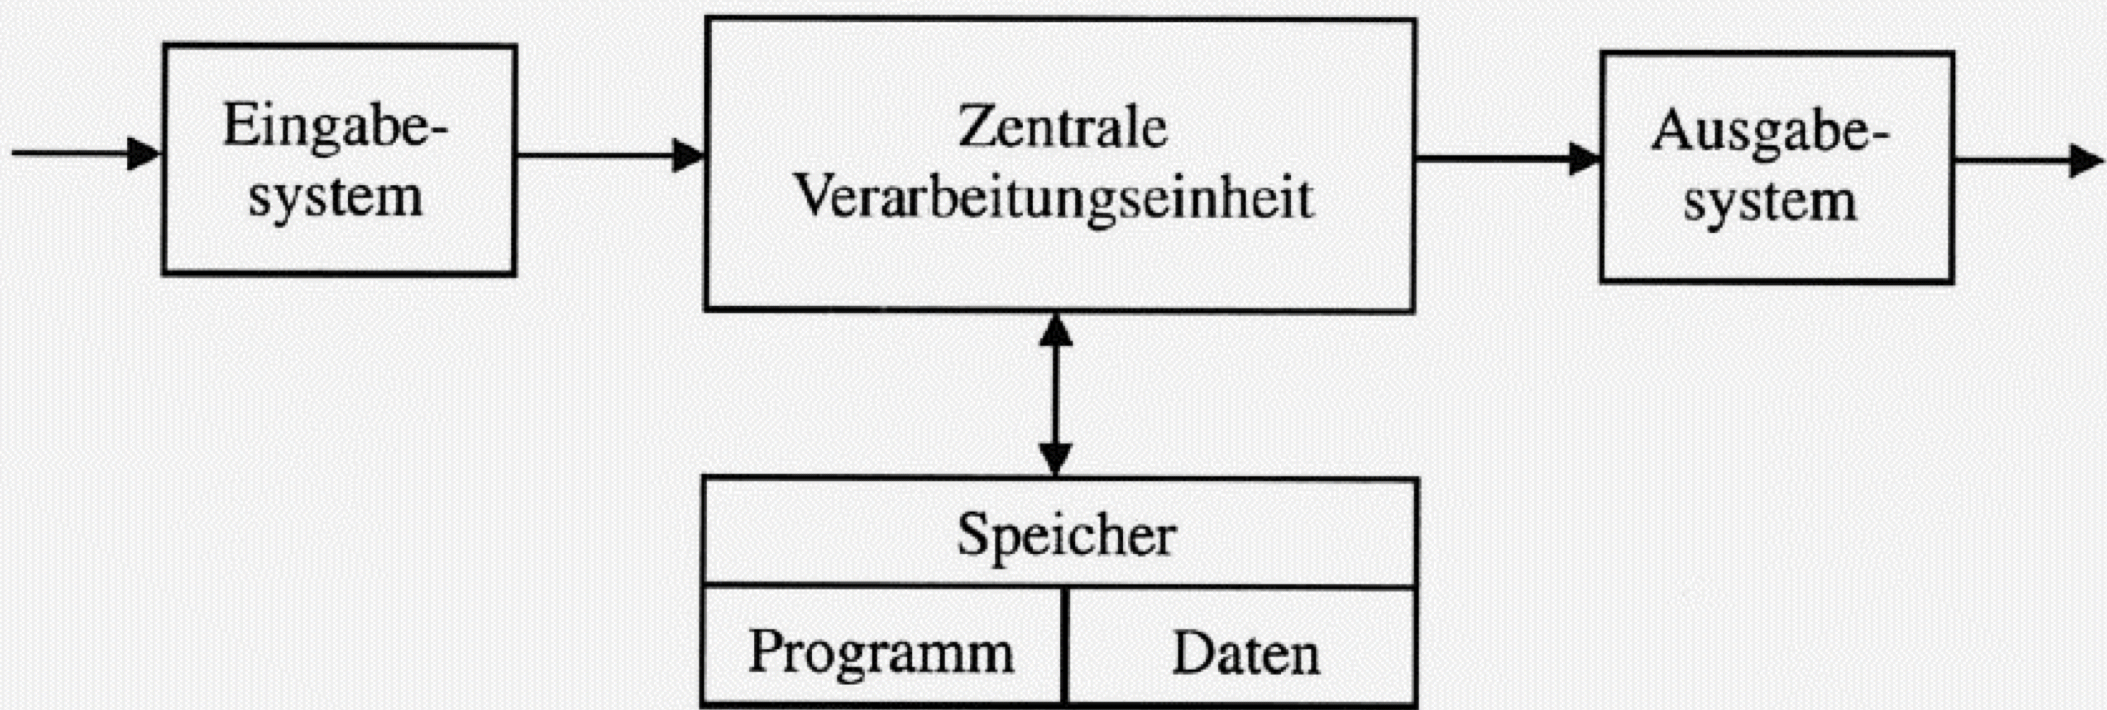
\includegraphics[width = 7cm]{pics/Datenverarbeitungsanlage}

\subsection{Moore's Law}
Moore's Law sagt aus, dass sich die Komplexit"at integrierter Schaltkreise regelm"assig verdoppelt, je nach Quelle werden 12 bis 24 Monate als Zeitraum genannt.

\subsection{Eingebettete Systeme}
\vspace{-4ex}
\begin{minipage}[c]{10cm}
\vspace{-2ex}
Heute sind weit "uber 90\% aller Computer als eingebettete Systeme realisiert, das heisst sie sind in Produkten wie zum Beispiel Haushaltsger"aten, Autos oder Fertigungszellen integriert.

Eingebettet Systeme (Embedded Systems) stellen stets ein Kombination aus Hard- und Softwarekomponenten dar, die in einem technischen Kontext (Prozess, Anlage) eingebunden sind.
\end{minipage}
%
\begin{minipage}{0.5cm}
	\ \
\end{minipage}
\begin{minipage}[c]{6cm}
	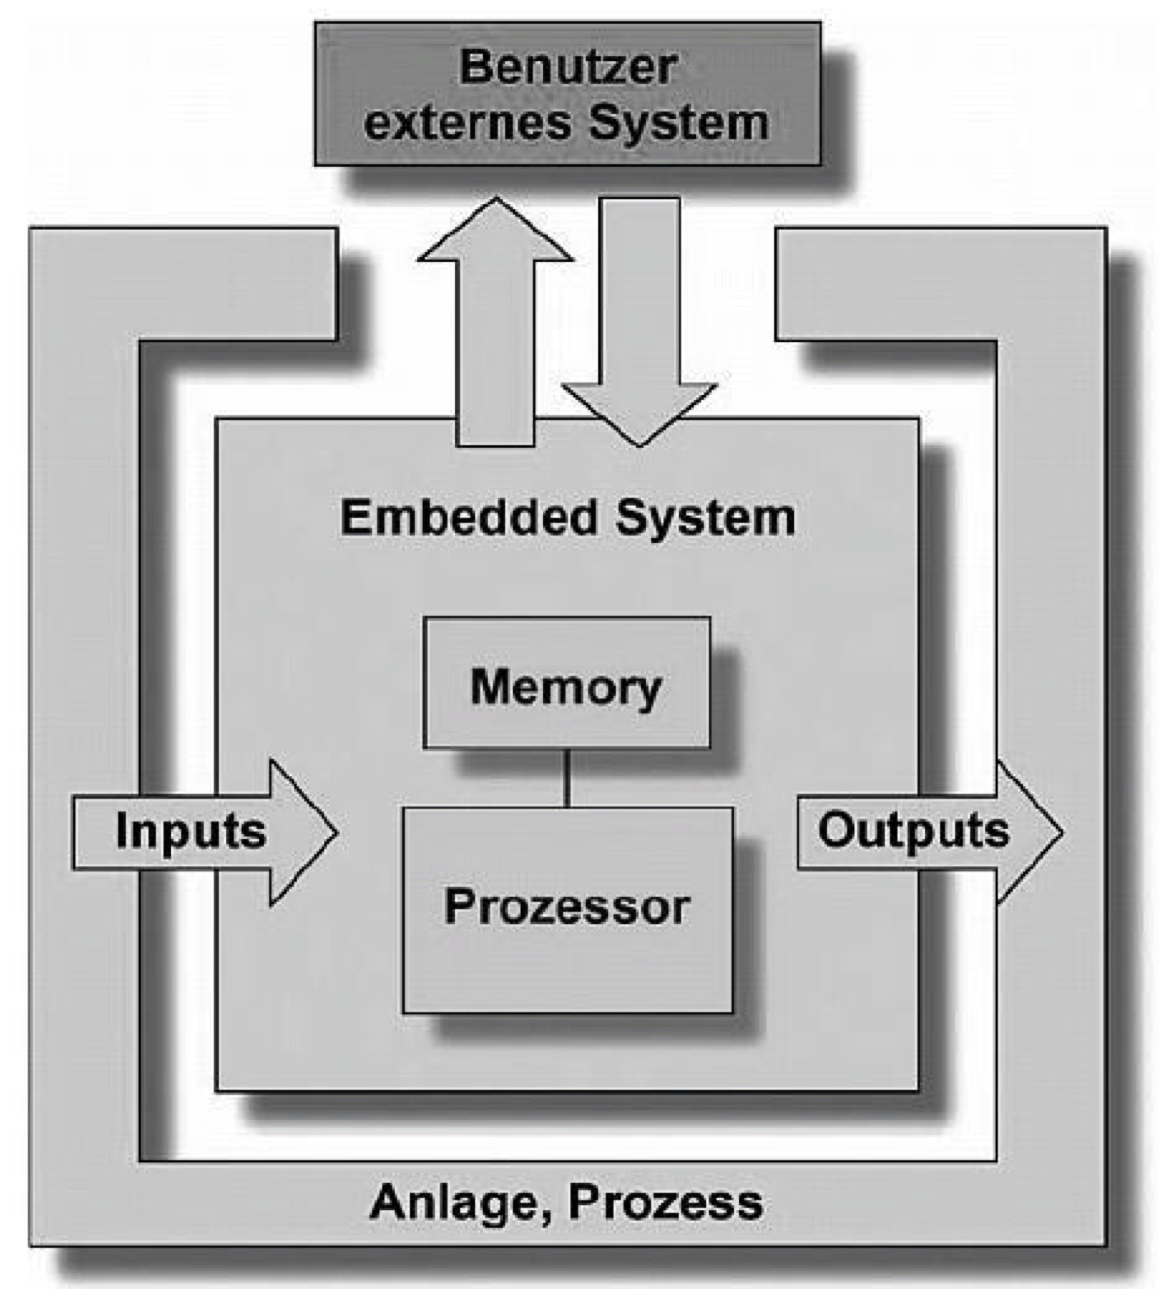
\includegraphics[width=3.5cm]{pics/Embedded-System}
\end{minipage}

\subsection{Bestandteile eine Mikrocomputers}
Ein Mikrocomputer besteht aus einer Zentraleinheit, aus Speicherelementen und aus Eingabe- und Ausgabe-Einheiten sowie aus einem Verbindungssystem.

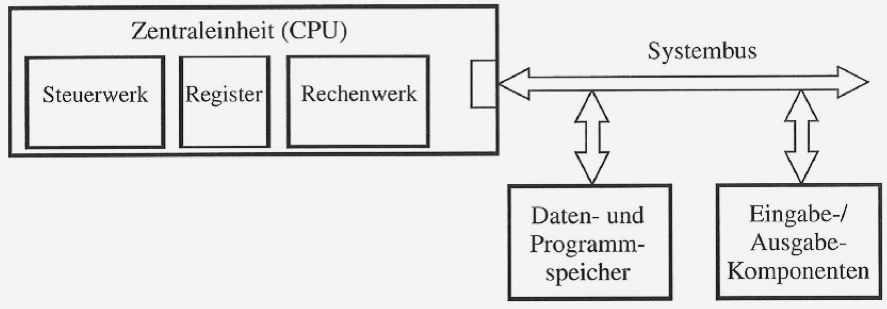
\includegraphics[width = 8cm]{pics/Mikrocomputer}

\begin{minipage}[t]{8.5cm}
	\subsubsection{CPU (Central Processing Unit)}
	Die CPU "ubernimmt als zentrale Berarbeitungseinheit die Datenverarbeitung als auch die Koordination aller computerinternen Aktivit"aten\\
	
	\subsubsection{Eingabe-/ Ausgabe-Einheiten}
	Sie dienen als Schnittstelle zur Aussenwelt. Die Anzahl und konkrete Konfiguration h"angt direkt vom Einsatz und Zweck ab.\\
	
	\subsubsection{Master-Slave-Prinzip}
	Die CPU steuert als Master aktiv alle Abl"aufe und Datentransporte. Speicher und periphere Komponenten arbeiten als Slave und werden normalerweise nur auf Aufforderung durch die CPU aktiv.
\end{minipage}
%
\begin{minipage}{1cm}
	\ \
\end{minipage}
%
\begin{minipage}[t]{8.5cm}
	\subsubsection{Speicher (Memory)}
	Der Speicher nimmt die zu verarbeitenden Daten, das Programm und weitere Informationen w"ahrend des gesamten Programmablaufs auf und stellt diese auf Anforderungen nach Bedarf zur Verf"ugung.\\
	
	\subsubsection{Systembus}
	Der Systembus dient als Verbindungszweig zwischen den Komponenten des Mikrocomputers. Prinzipiell funktioniert die Ablaufsteuerung auf dem Systembus nach einem Matser-Slave-Prinzip.\\
	
	\subsubsection{Interrupt-Konzept}
	Ist eine Erweiterung des Master-Slave-Prinzip, bei der periphere Slave-Einheiten eine Bedienungsanforderung (Interrupt-Request) bei der CPU anmelden k"onnen. Die CPU entscheidet "uber die Ber"ucksichtigung dieser Anforderung und den Zeitpunkt der Bearbeitung.
\end{minipage}

\subsection{Rechnerarchitekturen}
Die Art der Topologie (Zusammenschaltung) der verschiedenen Komponenten in einem Mikroprozessorsystem wird als Rechnerarchitektur bezeichnet.

\begin{minipage}{9cm}
	\subsubsection{Von-Neumann-Architektur}
Ein gemeinsamer Speicher f"ur Programme und Daten ist an einem Systembus angeschlossen. Damit steht nur ein Datenpfad f"ur Programm- und Dateninformationen zur Verf"ugung.

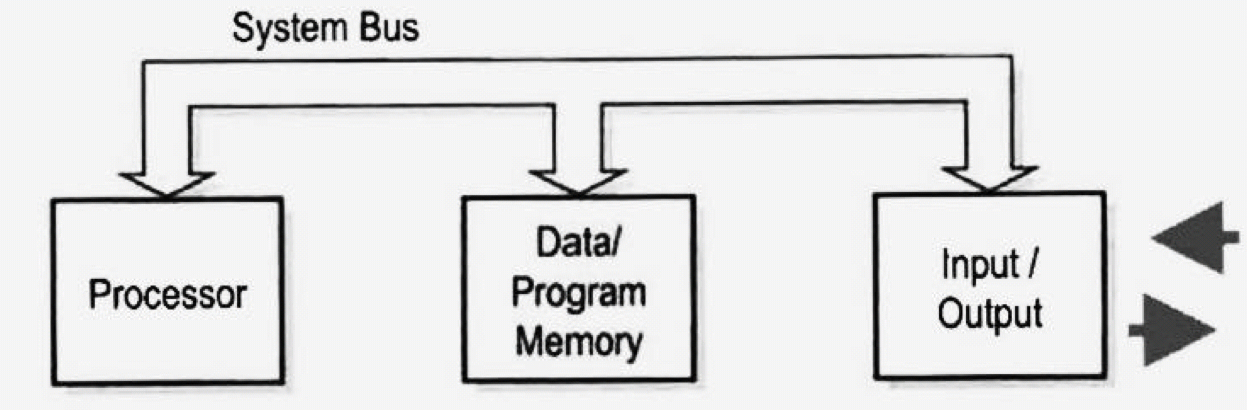
\includegraphics[width = 7cm]{pics/Von-Neumann-Architektur}
\end{minipage}
%
\begin{minipage}{0.5cm}
	\ \
\end{minipage}
%
\begin{minipage}{9cm}
	\subsubsection{Harvard-Architektur}
	Daten- und Programmspeicher sind getrennt ausgef"uhrt und "uber separate Busse an die CPU gekoppelt $\Rightarrow$ zeitgleiche "Ubertragung von Programm- und Dateninformationen.
	
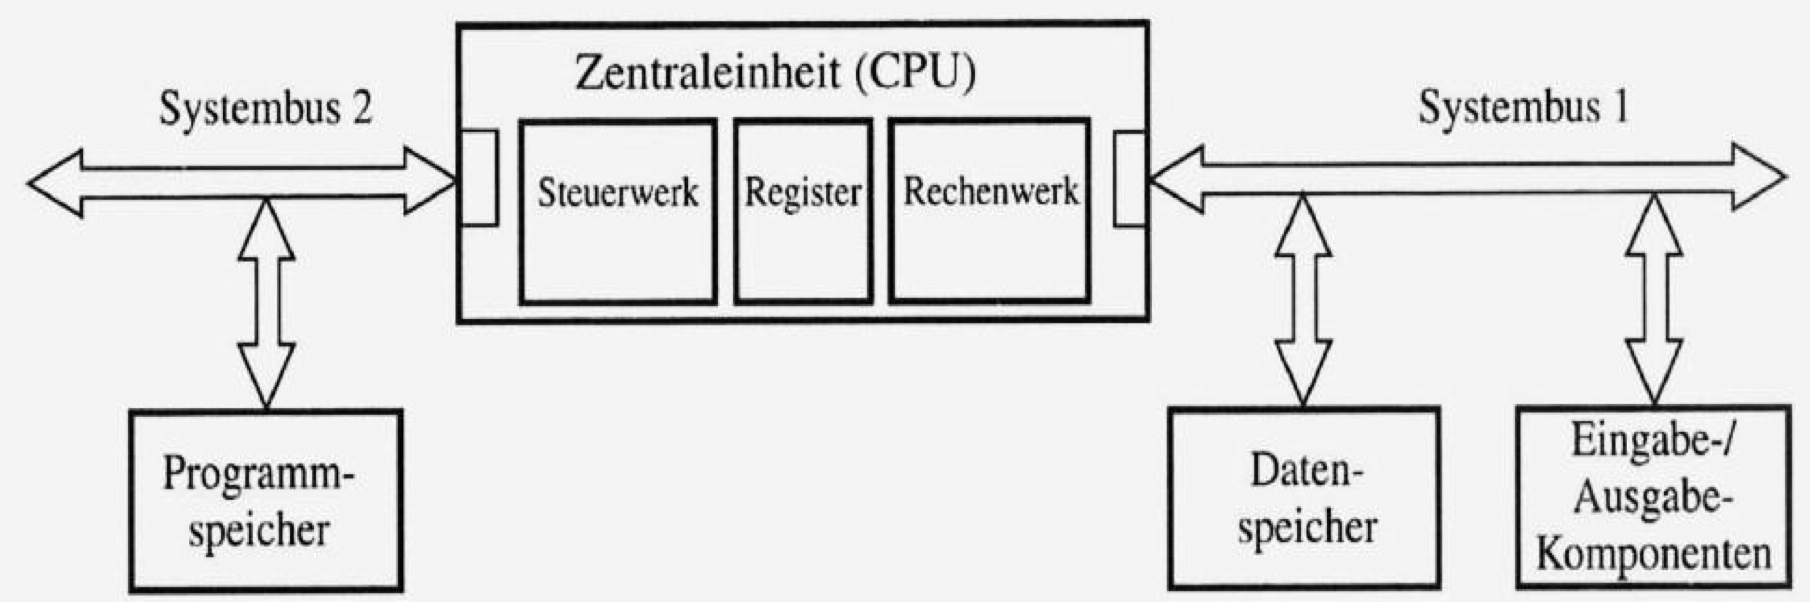
\includegraphics[width = 8cm]{pics/Harvard-Architektur}
\end{minipage}

\subsection{Mikroprozesssortechnik}
\begin{minipage}{11cm}
	Die \textbf{Mikroprozessortechnik} befasst sich mit der Architektur, der Entwicklung, der Implementierung, dem Bau, der Programmierung und dem Einsatz von Mikroprozessoren.

Ein \textbf{Mikroprozessor} ($\mu$P) ist die auf einem Chip realisierte CPU eines Computersystems.

Eine \textbf{Mikroarchitektur} bezeichnet die Implementierung einer Prozessorarchitektur ein einer speziellen Verk"orperung der Architektur - also in einem Mikroprozessor.
\end{minipage}
%
\begin{minipage}{0.5cm}
	\ \
\end{minipage}
%
\begin{minipage}{7cm}
	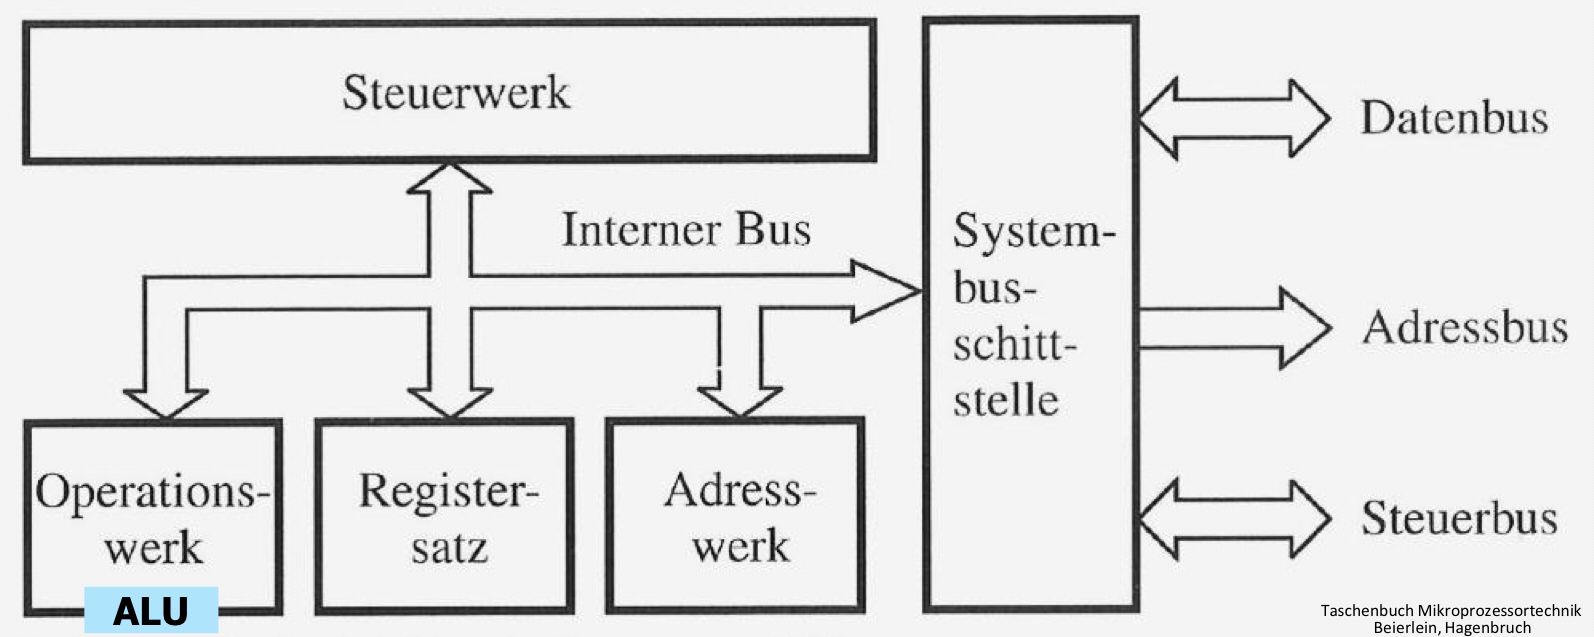
\includegraphics[width=7cm]{pics/CPU}
\end{minipage}

\subsection{Differenzierung von Mikroprozessoren}
Mikroprozessoren unterscheiden sich durch zahlreiche Parameter und Architekturmerkmale. Es gibt f"unf Hauptgruppen.
\textbf{Standard-Mikroprozessoren} sind f"ur den allgemeinen Einsatz z.B. f"ur Drucker, Workstations usw.

\textbf{Hochleistungs-Mikroprozessoren} f"ur Computer mit sehr hoher Verarbeitungsleistung (z.B. f"ur Grossrechner, Netzwerkkomponenten)

\begin{minipage}{9cm}
\subsubsection{Mikrocontroller ($\mu$C)}
	Mikrokontroller sind vollst"andige Mikrorechnersysteme auf einem Chip. Sie beinhalten Speicher Peripherien, CPU und Speicher.
	Sie werden f"ur Automatisierungen, f"ur die Medizintechnik und f"ur viele weitere Sachen verwendet.\\
	\end{minipage}
%
\begin{minipage}{0.5cm}
	\ \
\end{minipage}
%
\begin{minipage}{9cm}
	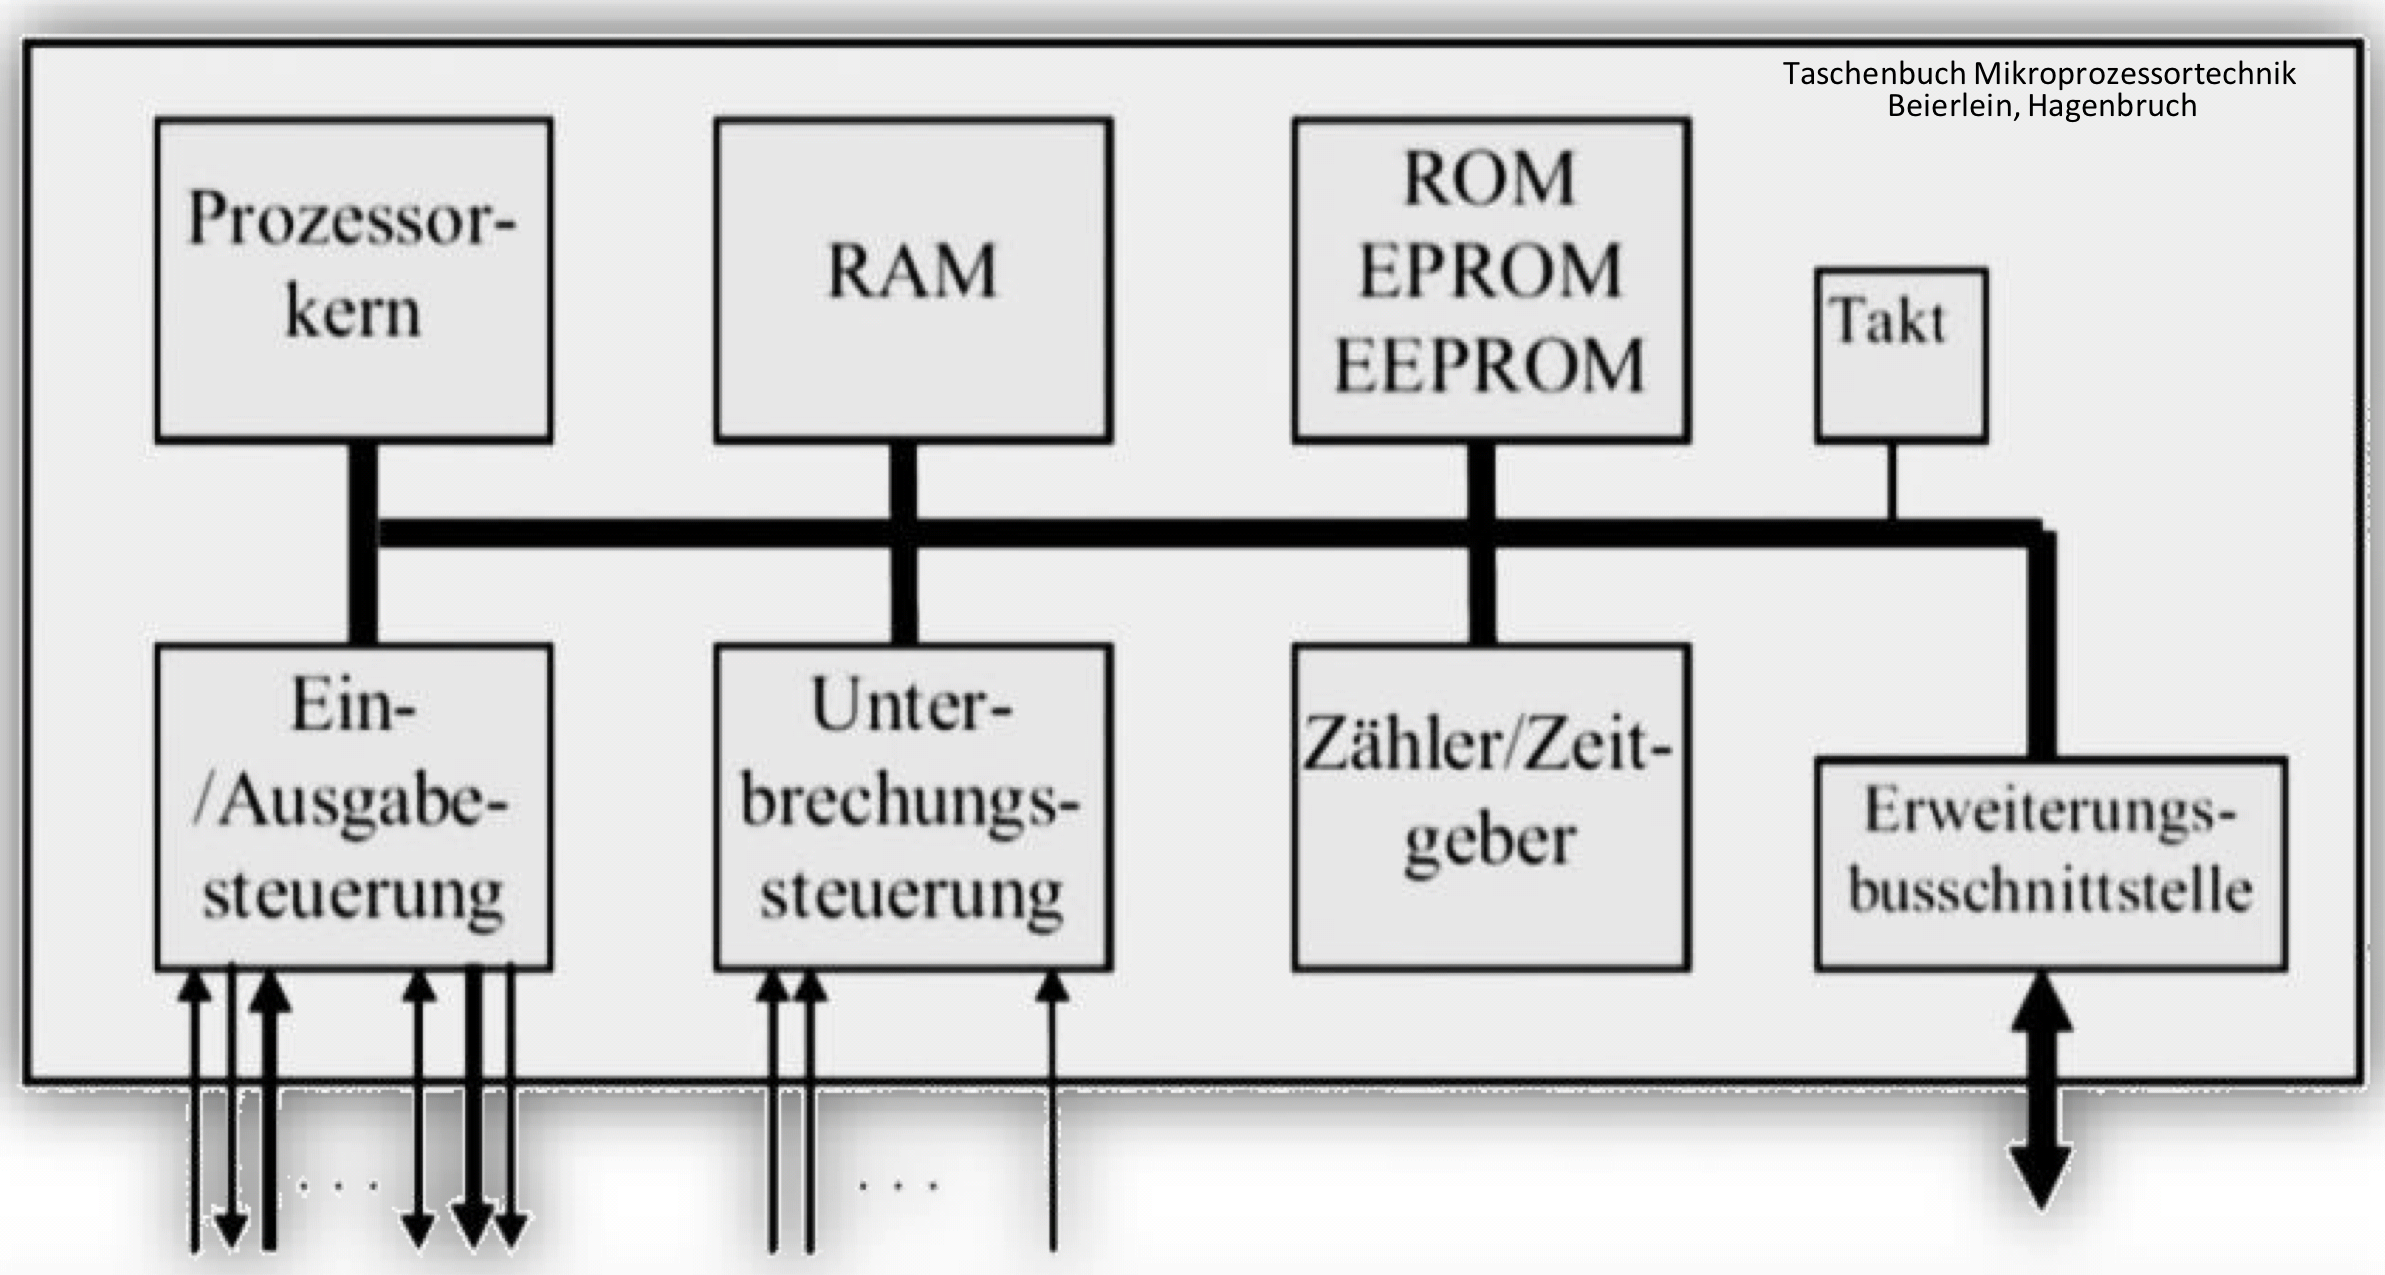
\includegraphics[width=5cm]{pics/Mikrokontroller}
\end{minipage}

\begin{minipage}{9cm}
	\subsubsection{Digitale Signalprozessoren (DSP)}
	Digitale Signalprozessoren sind Mikroprozessoren welche f"ur die schnelle Verarbeitung von mathematischen Befehle und f"ur die Bearbeitung komplexer Algorithmen von digitalisierten Analogsignalen optimiert sind.
\end{minipage}
%
\begin{minipage}{0.5cm}
	\ \
\end{minipage}
%
\begin{minipage}{9cm}
	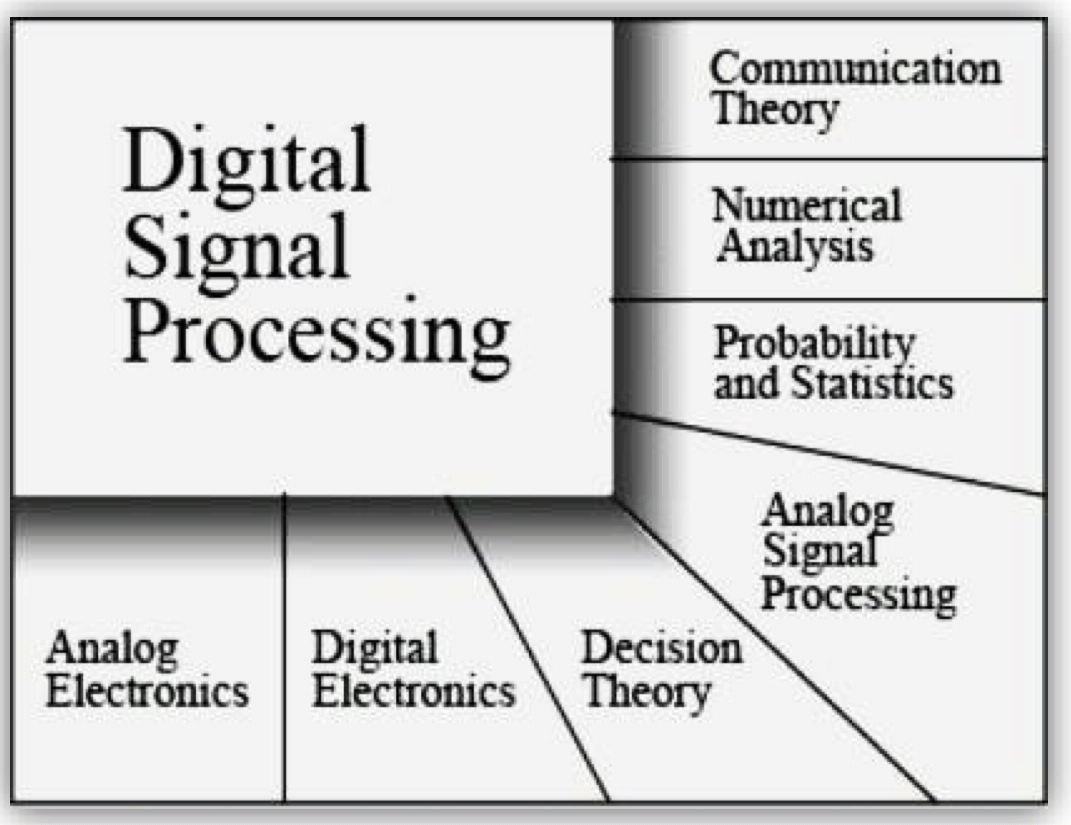
\includegraphics[width=3cm]{pics/Digitale-Signalprozessoren}
\end{minipage}

\subsubsection{Software-Prozessorkern}
	F"ur \textbf{ASIC} (Application-Specific Integrated Circuit) und \textbf{FPGA} (Field Programmable Gate Array) stehen zahlreiche CPU-Designs in Form von Software-Bibliotheken zur Verf"ugung. Solche Software-Prozessorkerne (Soft-Core) erm"oglichen die Realisierung kompletter Systeme auf einem Chip.

\textbf{Systems on Chip} (SoC) sind komplexe Systeme, die eine oder mehrere Verarbeitungseinheiten (CPUs), Programm- und Datenspeicher sowie vielf"altige analoge und digitale Funktionseinheiten auf einem Chip enthalten.

Als \textbf{SoPC} (System-on-Programmable-Chip) bezeichnet die Technologie, ein SoC nicht auf einem ASIC sondern mittels eines programmierbaren Hardware-Bausteins (z.B. FPGA) zu realisieren.

\subsection{Ausgew"ahlte Architekturmerkmale}
\begin{minipage}{14.5cm}
	Das \textbf{Programmiermodell} fasst wichtige Teile der Mikroprozessorarchitektur zusammen und spiegelt die Struktur des Prozessors wieder.

	Bei der Speicheradressierung gibt es das \textbf{Big-Endian- /Little-Endian-Format}, wobei bei der Little-Endian-Formatierung das LSB die Startadresse festlegt und bei der Big-Endian-Formatierung legt das MSB die Startadresse fest.

	Zudem gibt es noch weitere Architekturmerkmale wie Programmierbarkeit des Systemtaktes, ausf"uhrung der Recheneinheit, Taktfrequenz, Cache-Speicher On-CHip, Konfigurierbarkeit von Komponenten des Mikroprozessors usw.
\end{minipage}
%
\begin{minipage}{0.5cm}
	\ \
\end{minipage}
%
\begin{minipage}{4cm}
	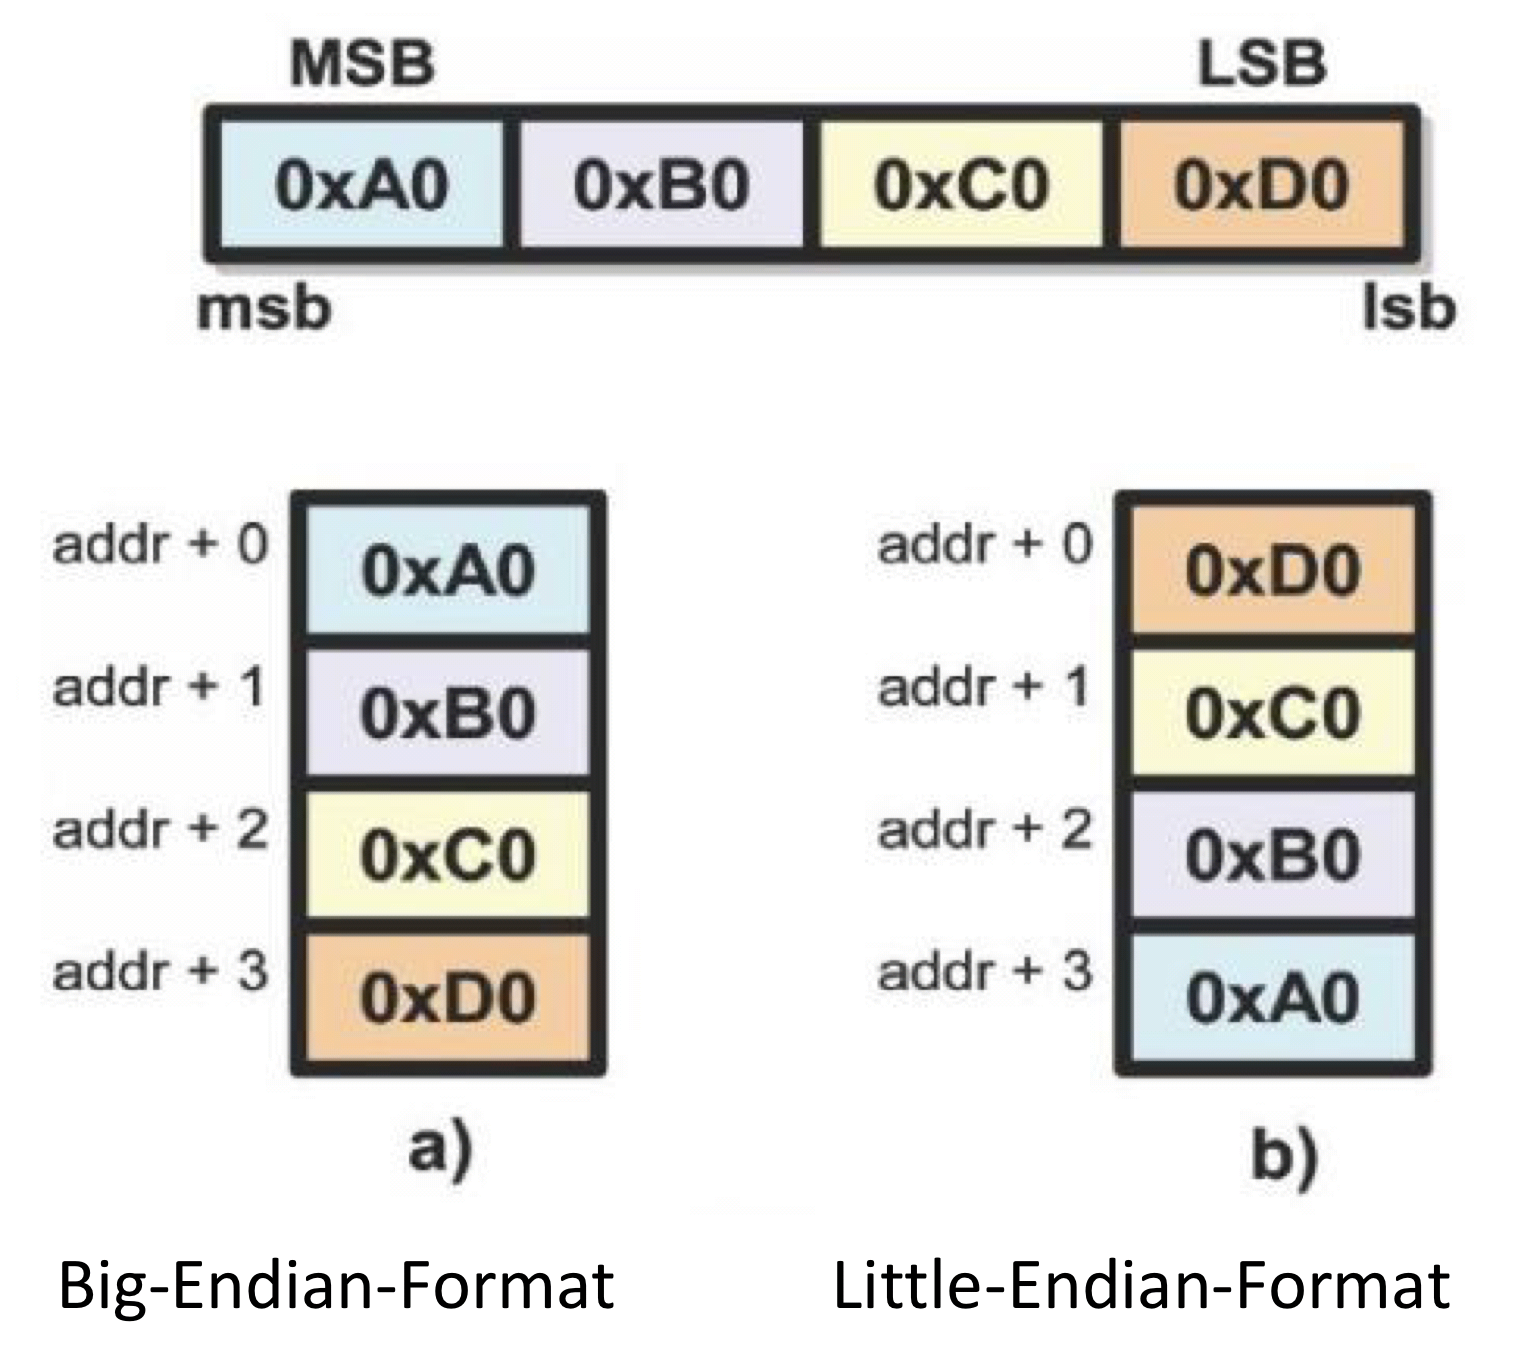
\includegraphics[width=4cm]{pics/Big-Endian_Little-Endian}
\end{minipage}



	\section{Informationsdarstellung}
\subsection{Begriffe und Definitionen}

\begin{minipage}[t]{9cm}
	\subsubsection{Maschinenwort}
	Das Maschinenwort ist die endliche geordnete Folge von Bin"arzeichen, die im Computer als Einheit verarbeitet werden kann. Es entspricht der Gr"osse des Rechenwerks und wird auch \dq Word\dq \ \ genannt.
	
	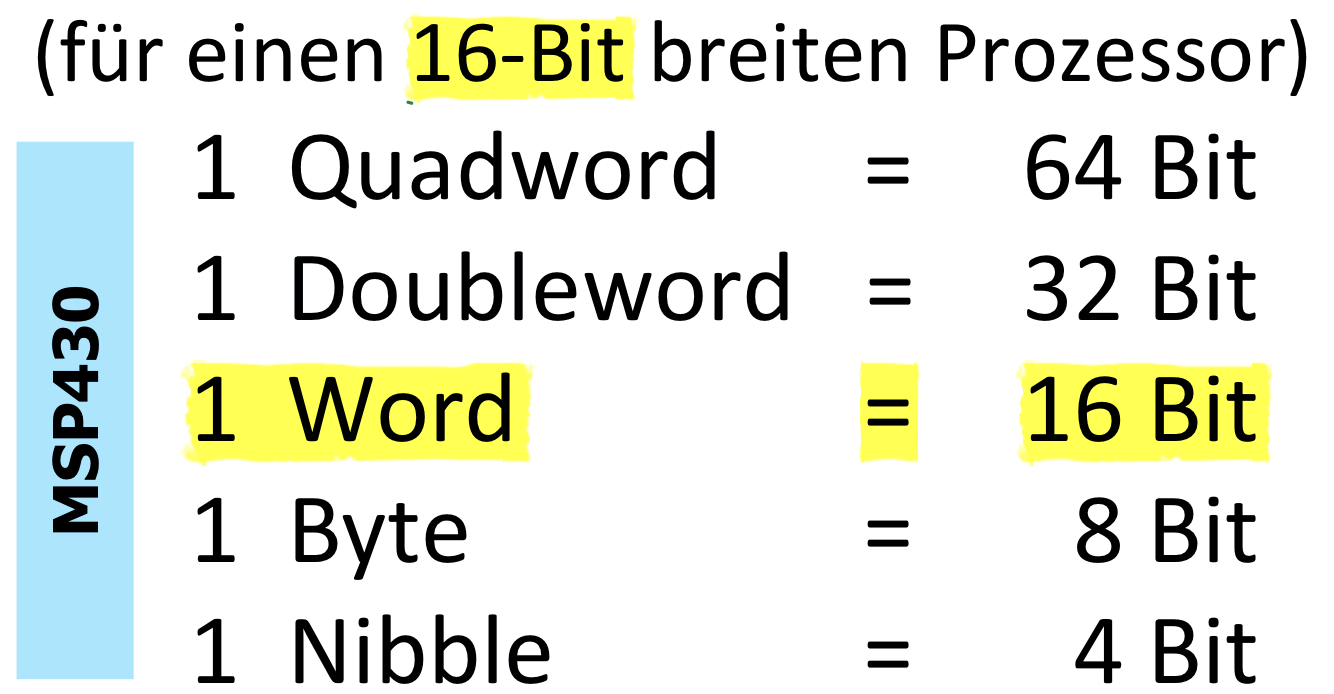
\includegraphics[width = 5cm]{pics/Wortlaenge}

	\subsubsection{Informationsparameter (Signal Parameter)}
	Die Kenngr"osse eines Signals, dessen Wert die Information beinhaltet.
	Bie einer Wechselspannung w"are das zum Beispiel die Amplitude, die Frequenz oder der Phasenwinkel.

\end{minipage}
%
\begin{minipage}{0.5cm}
	\ \
\end{minipage}
%
\begin{minipage}[t]{9cm}
	\subsubsection{Signalarten}
	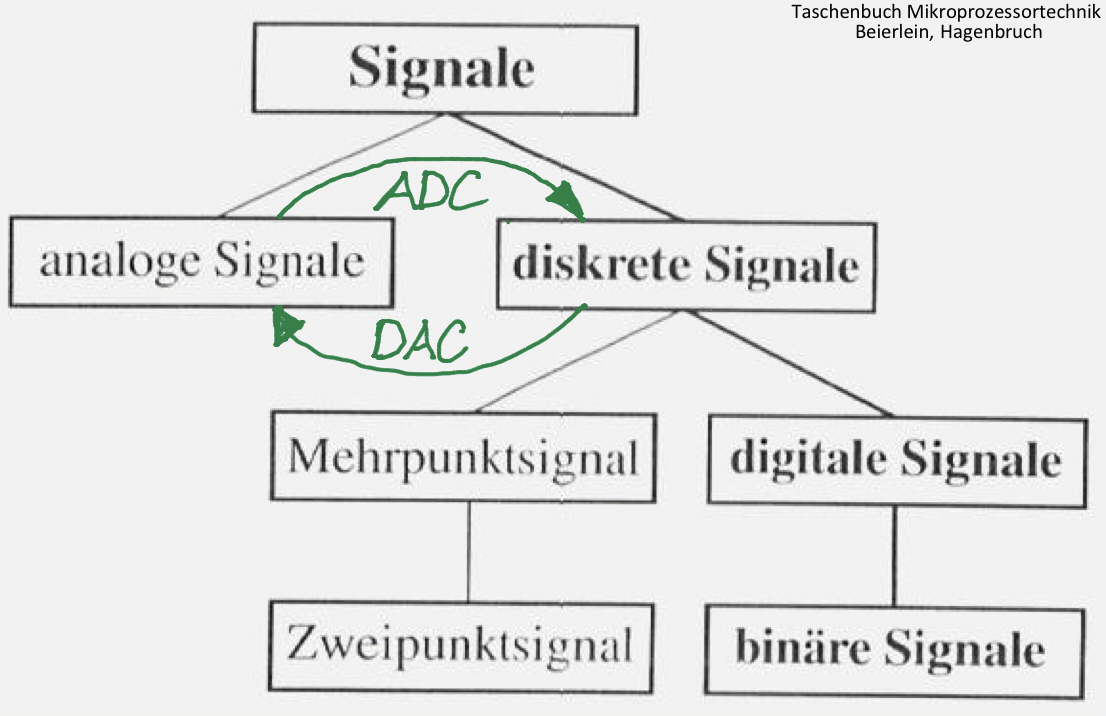
\includegraphics[width=8cm]{pics/Signalarten}
\end{minipage}

\begin{minipage}[t]{9cm}
\ \
	\subsection{Grundlegende Datenarten}
	Sowohl auf der Input- wie auch auf der Output-Seite werden drei verschiedene, grundlegende Datenarten unterschieden:
	
	\textbf{Signale}, welche beim Auftreten eines Ereignisses Information liefern, sind Zeitlich zuf"allig

	\textbf{Daten-Meldungen} liefern Daten, welche Informationen enthalten, auch zu einem zuf"alligen Zeitpunkt.

	\textbf{Datenstr"ome} m"ussen periodisch abgetastet, "ubertragen und in der gleichen sequenziellen Reihenfolge verarbeitet werden.
	
	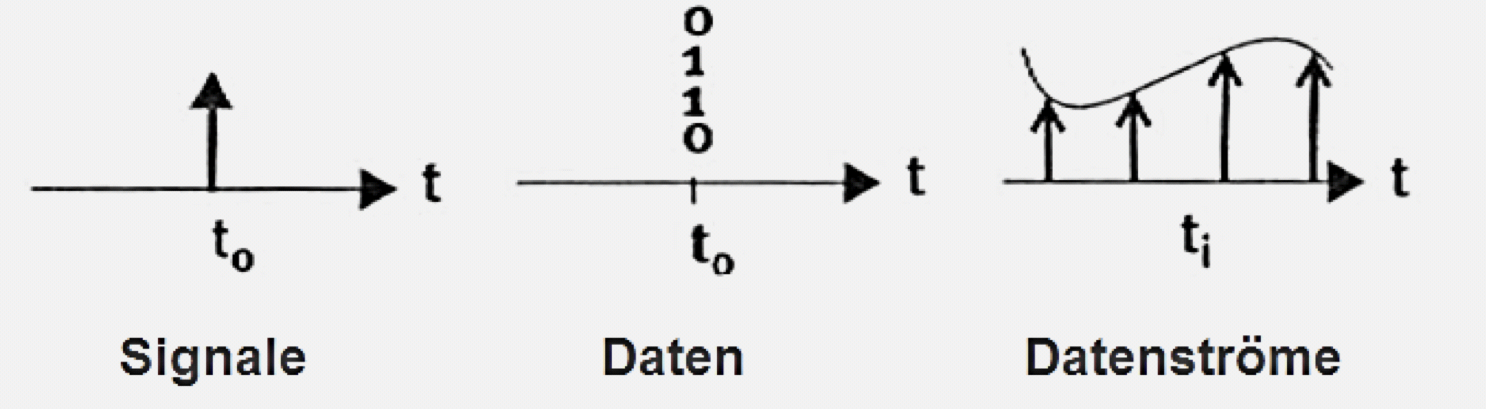
\includegraphics[width=6cm]{pics/Datenarten}
	
	\subsection{Gr"ossen-Angaben bei Speichern}
	Auf das Bin"arsystem bezogen werden die Bezeichnungen Kilo(K), Mega(M) und Giga (G) verwendet, damit es keine Verwechslung gibt, denn: \textbf{1K $\neq$ 1k = $10^3$}

	\textbf{1K} = $2^{10}$ = 1024\\
	\textbf{1M} = 1024K = 1048576\\
	\textbf{1G} = 1024M
	\end{minipage}
%
\begin{minipage}{0.5cm}
	\ \
\end{minipage}
%
\begin{minipage}[t]{9cm}
\ \
	\subsection{ASCII-Code}
	Die Kodierung eines Zeichen setzt sich aus sieben Bits zusammen. Neben Zeichen gibt es auch noch Steuerfunktionen. Die Kodierung eines Zeichens setzt sich folglich zusammen: \dq 0x Spaltenindex Zeilenindex\dq  (z.B. \dq V\dq = 0x56)
	
	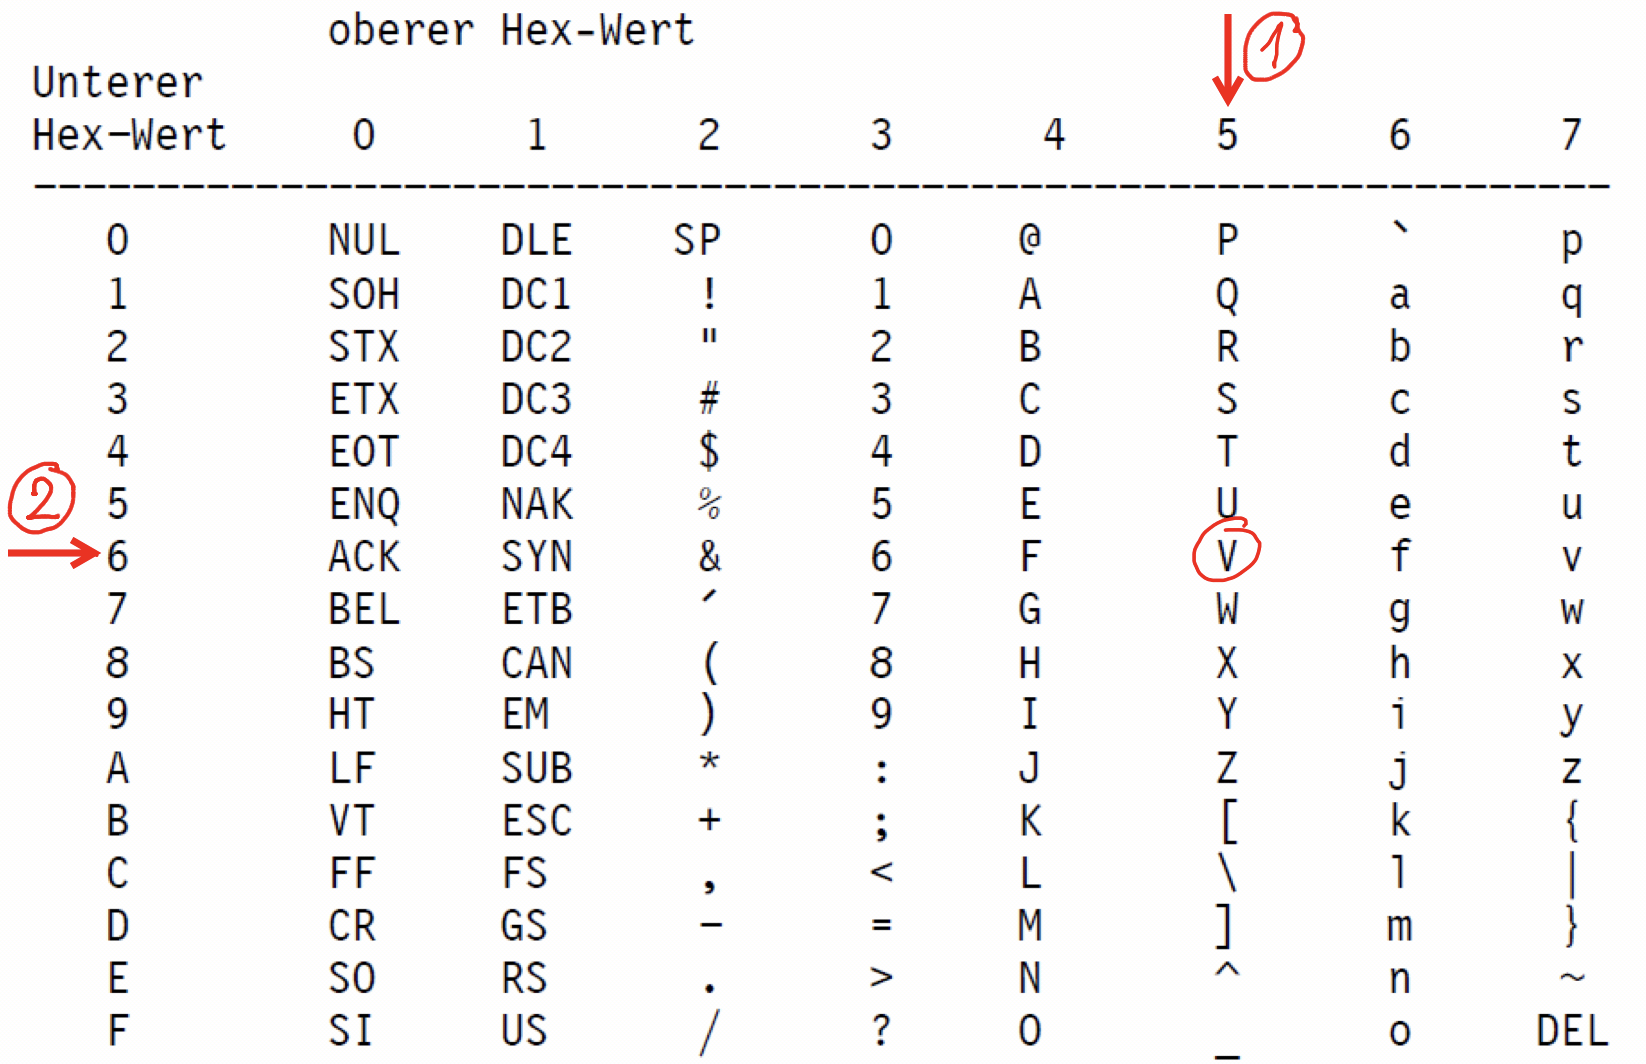
\includegraphics[width=9cm]{pics/ASCII-Tabelle}
\end{minipage}

\subsection{Zahlensysteme}
Zwischen dem Dezimal-, Bin"ar-, Oktal- und Hexadezimalsystem k"onne die Zahlen relativ einfach umgerechnet werden. Eine Zahl im \textbf{Bin"arsystem} wird \textbf{\%} gekennzeichnet, eine Zahl im \textbf{Oktalsystem} mit \textbf{@} und eine Zahl im \textbf{Hexadezimalsystem} mit \textbf{0x}.


\subsubsection{Umrechnung Dezimal $\Leftrightarrow$ Bin"ar $\Leftrightarrow$ Hex}
\begin{minipage}{7cm}
	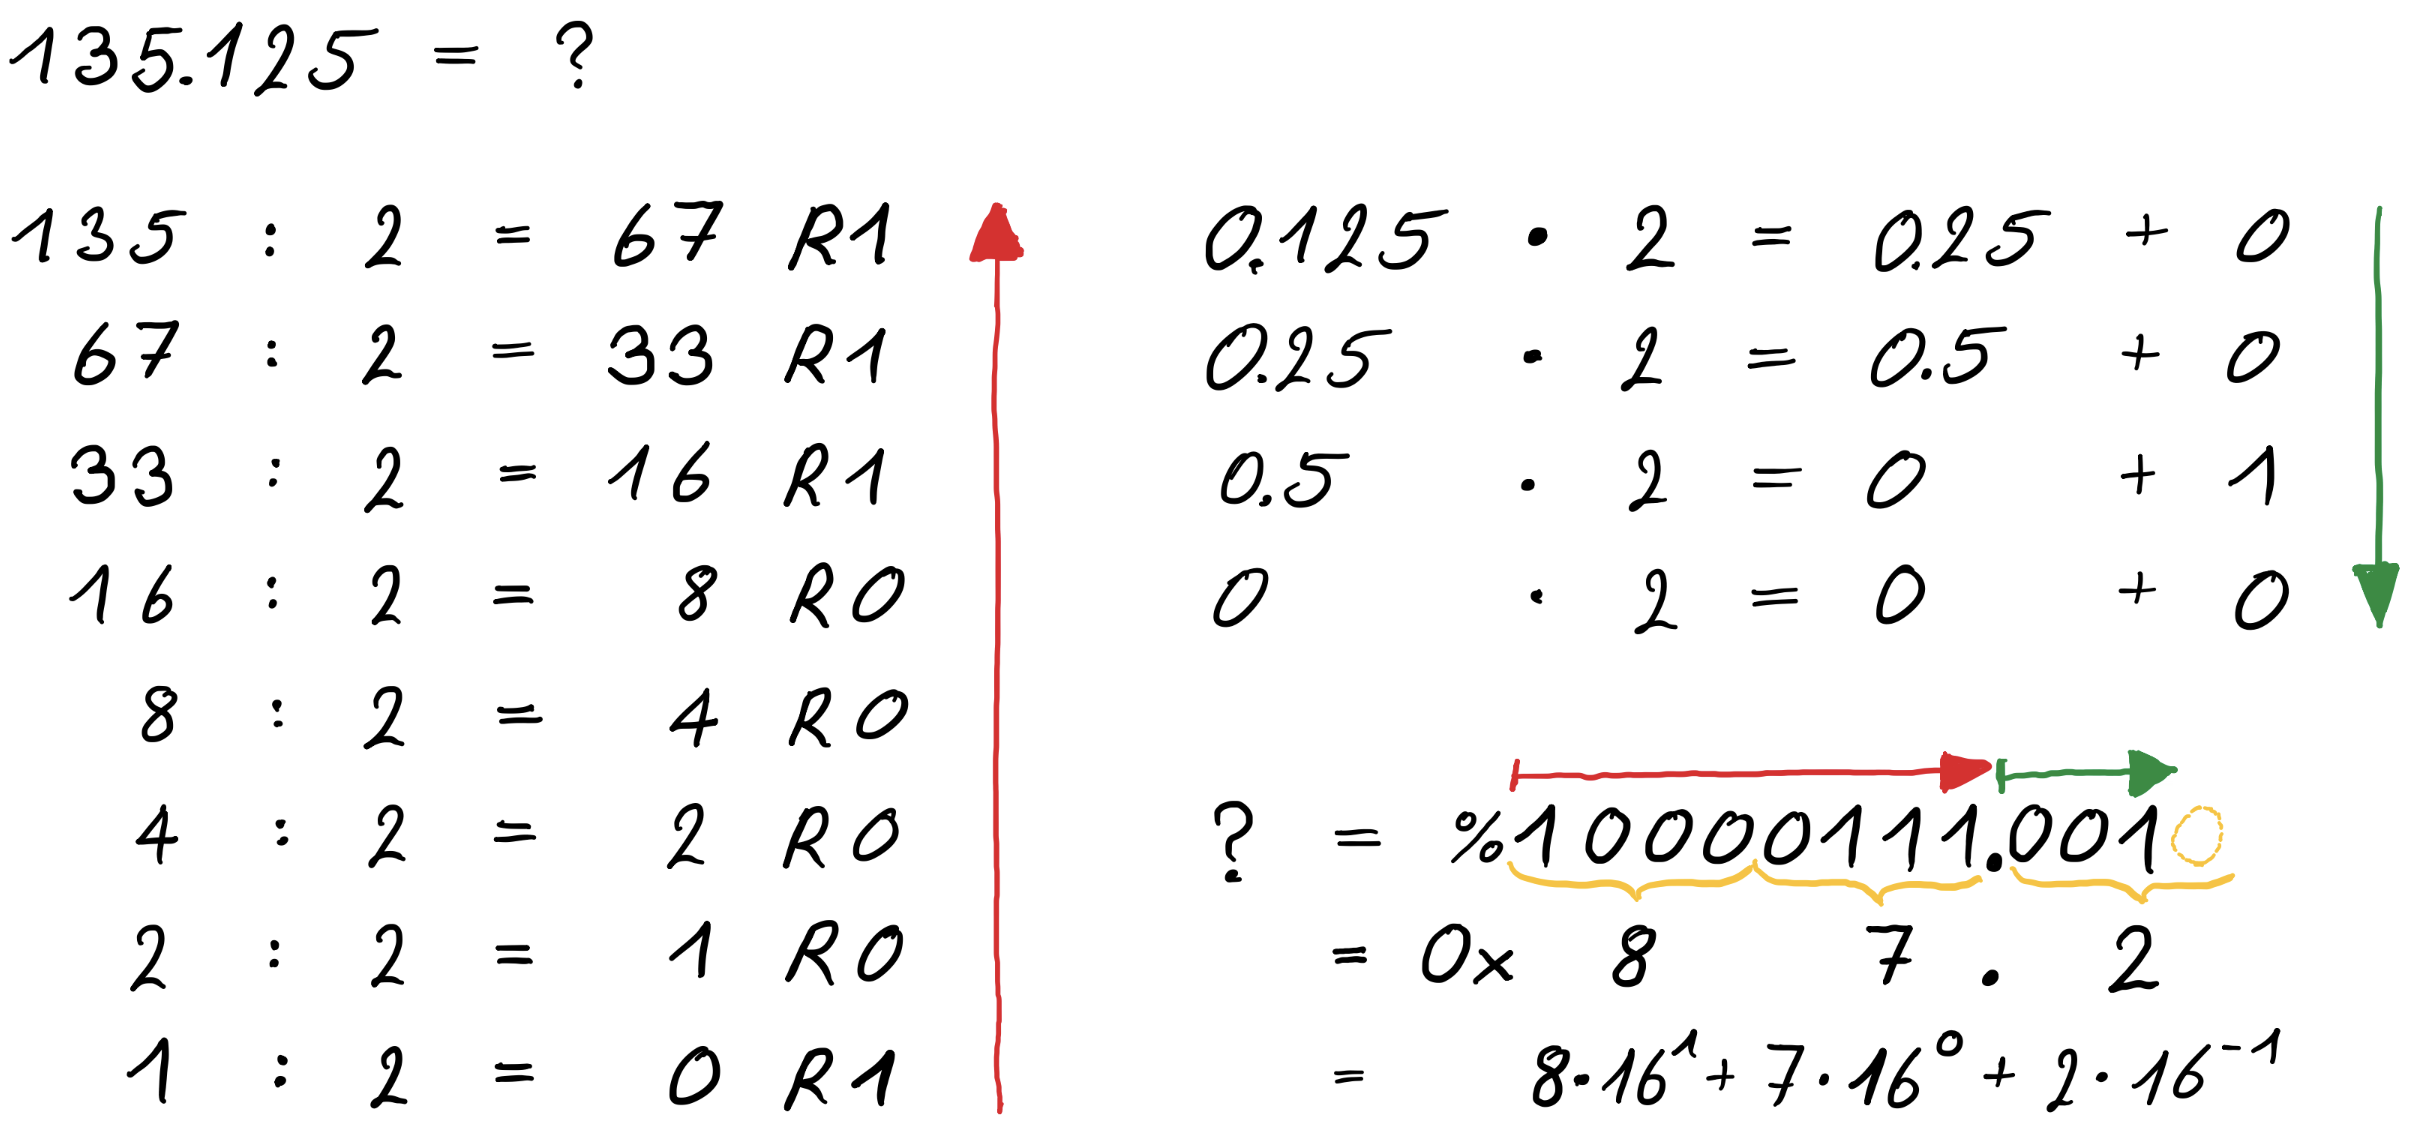
\includegraphics[width=7cm]{pics/Zahlenumrechnung}
\end{minipage}
%
\begin{minipage}{0.5cm}
	\ \
\end{minipage}
%
\begin{minipage}{11cm}
	Wenn die Bin"arzahl statt ins Hexadezimale ins \textbf{Oktalsystem} gewandelt werden soll, m"ussen statt Viererpakete Dreierpakete geb"undelt werden. 
	
	Soll eine Zahl in \textbf{BCD-Code} konvertiert werden, dann bekommt jede Ziffer der Dezimalzahl ein Nibble, mit dem Wert der Ziffer.
\end{minipage}


\begin{minipage}[t]{10cm}
	\vspace{-4ex}
	\subsubsection{Vorzeichenlose Ganzzahlen (unsigned integer)}
	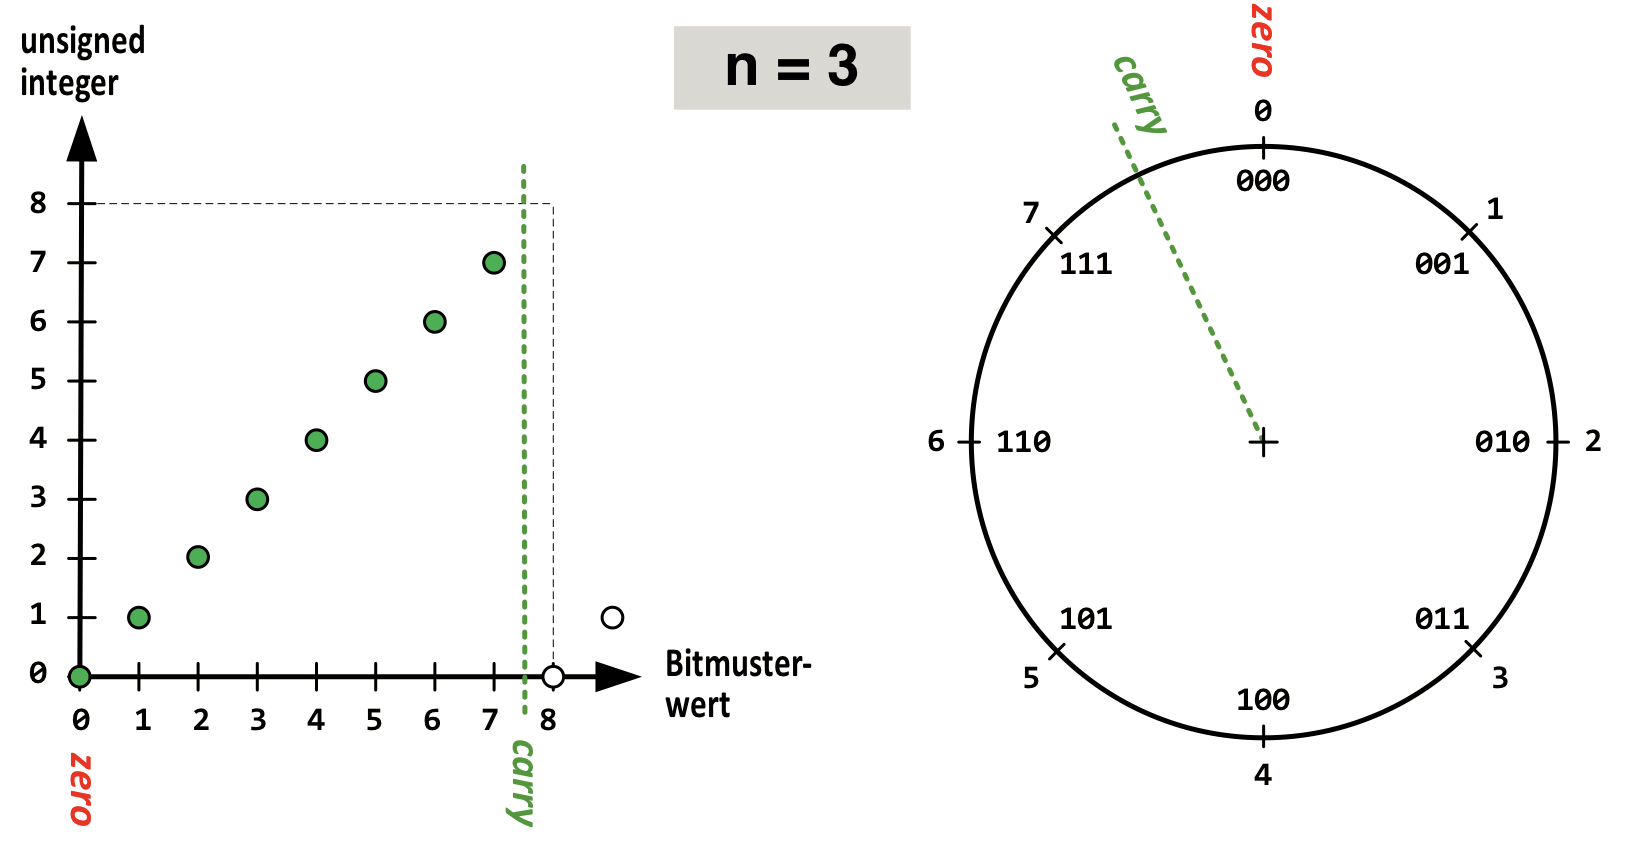
\includegraphics[width=7cm]{pics/Unsigned-Zahl}
	
	Vorzeichenlose Ganzzahlen, auch unsigned integer Zahlen gennant, k"onnen nur positive ganzzahlige Werte annehmen.
	\begin{tabbing}
		\textbf{Ca}\= \textbf{rry-Flag:}\\
		\> Wenn $a + b > 2^n -1$, dann wird das Carry-Flag gesetzt\\
		\> Wenn $a - b$ und $b > a$, dann wird auch das Carry-Flag\\
		\> gesetzt,in diesem Fall nennt man es auch \textbf{borrow}.\\

		\textbf{Zero-Flag:}\\
		\> Wenn das Resultat 0, Zero ergibt, dann wird das Zero-Flag\\ 
		\> gesetzt.
	\end{tabbing}

	\subsubsection{Zweierkomplement (signed integer)}
	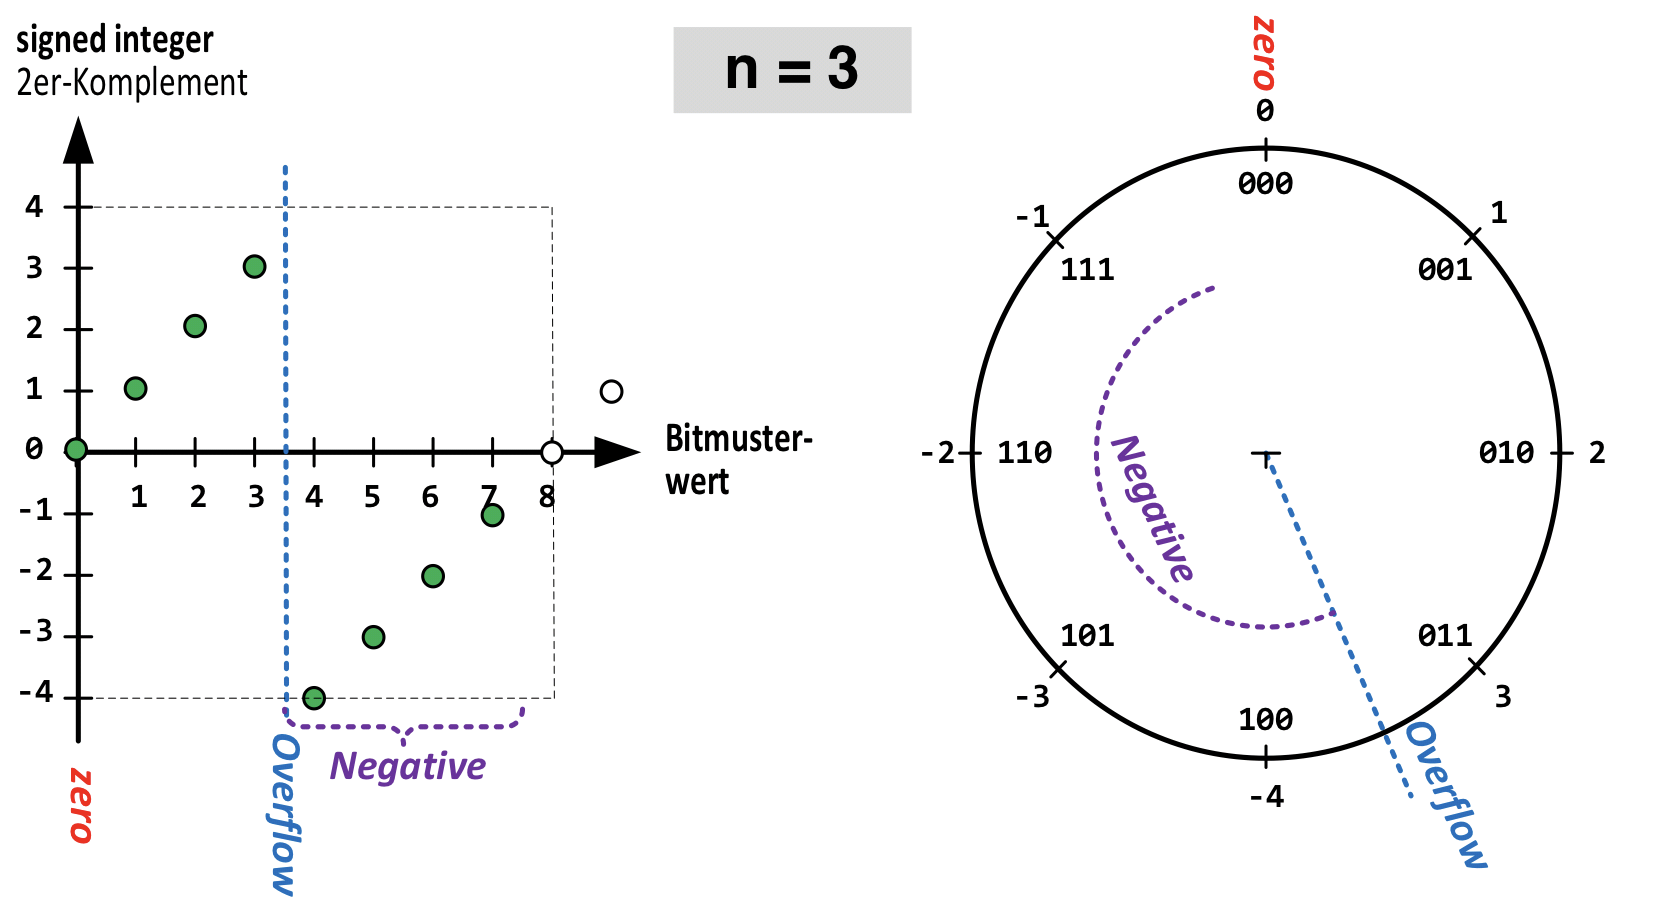
\includegraphics[width=7cm]{pics/Signed-Zahl}
	
	Vorzeichenbehaftete Ganzzahlen, auch signed integer Zahlen gennant, k"onnen positive und negative Ganzzahlwerte annehmen.
	\vspace{-2ex}
	\begin{tabbing}
		\textbf{Ne}\= \textbf{gative-Flag:}\\
		\> Wenn sich die Zahl im negativen Bereich des Zahlenkreises\\ 
		\> befindet wird das Negative-Flag gesetzt.\\

		\textbf{Overflow-Flag:}\\
		\> Wenn die Addition oder Subtraktion rein mathematisch keinen\\ 
		\> Sinn ergibt und der Overflow-Bereich auf dem Zahlenkreis\\
		\> "uberschritten wird, wird das Overflow-Flag gesetzt.
	\end{tabbing}

	\subsubsection{Duales Rechenwerk}
	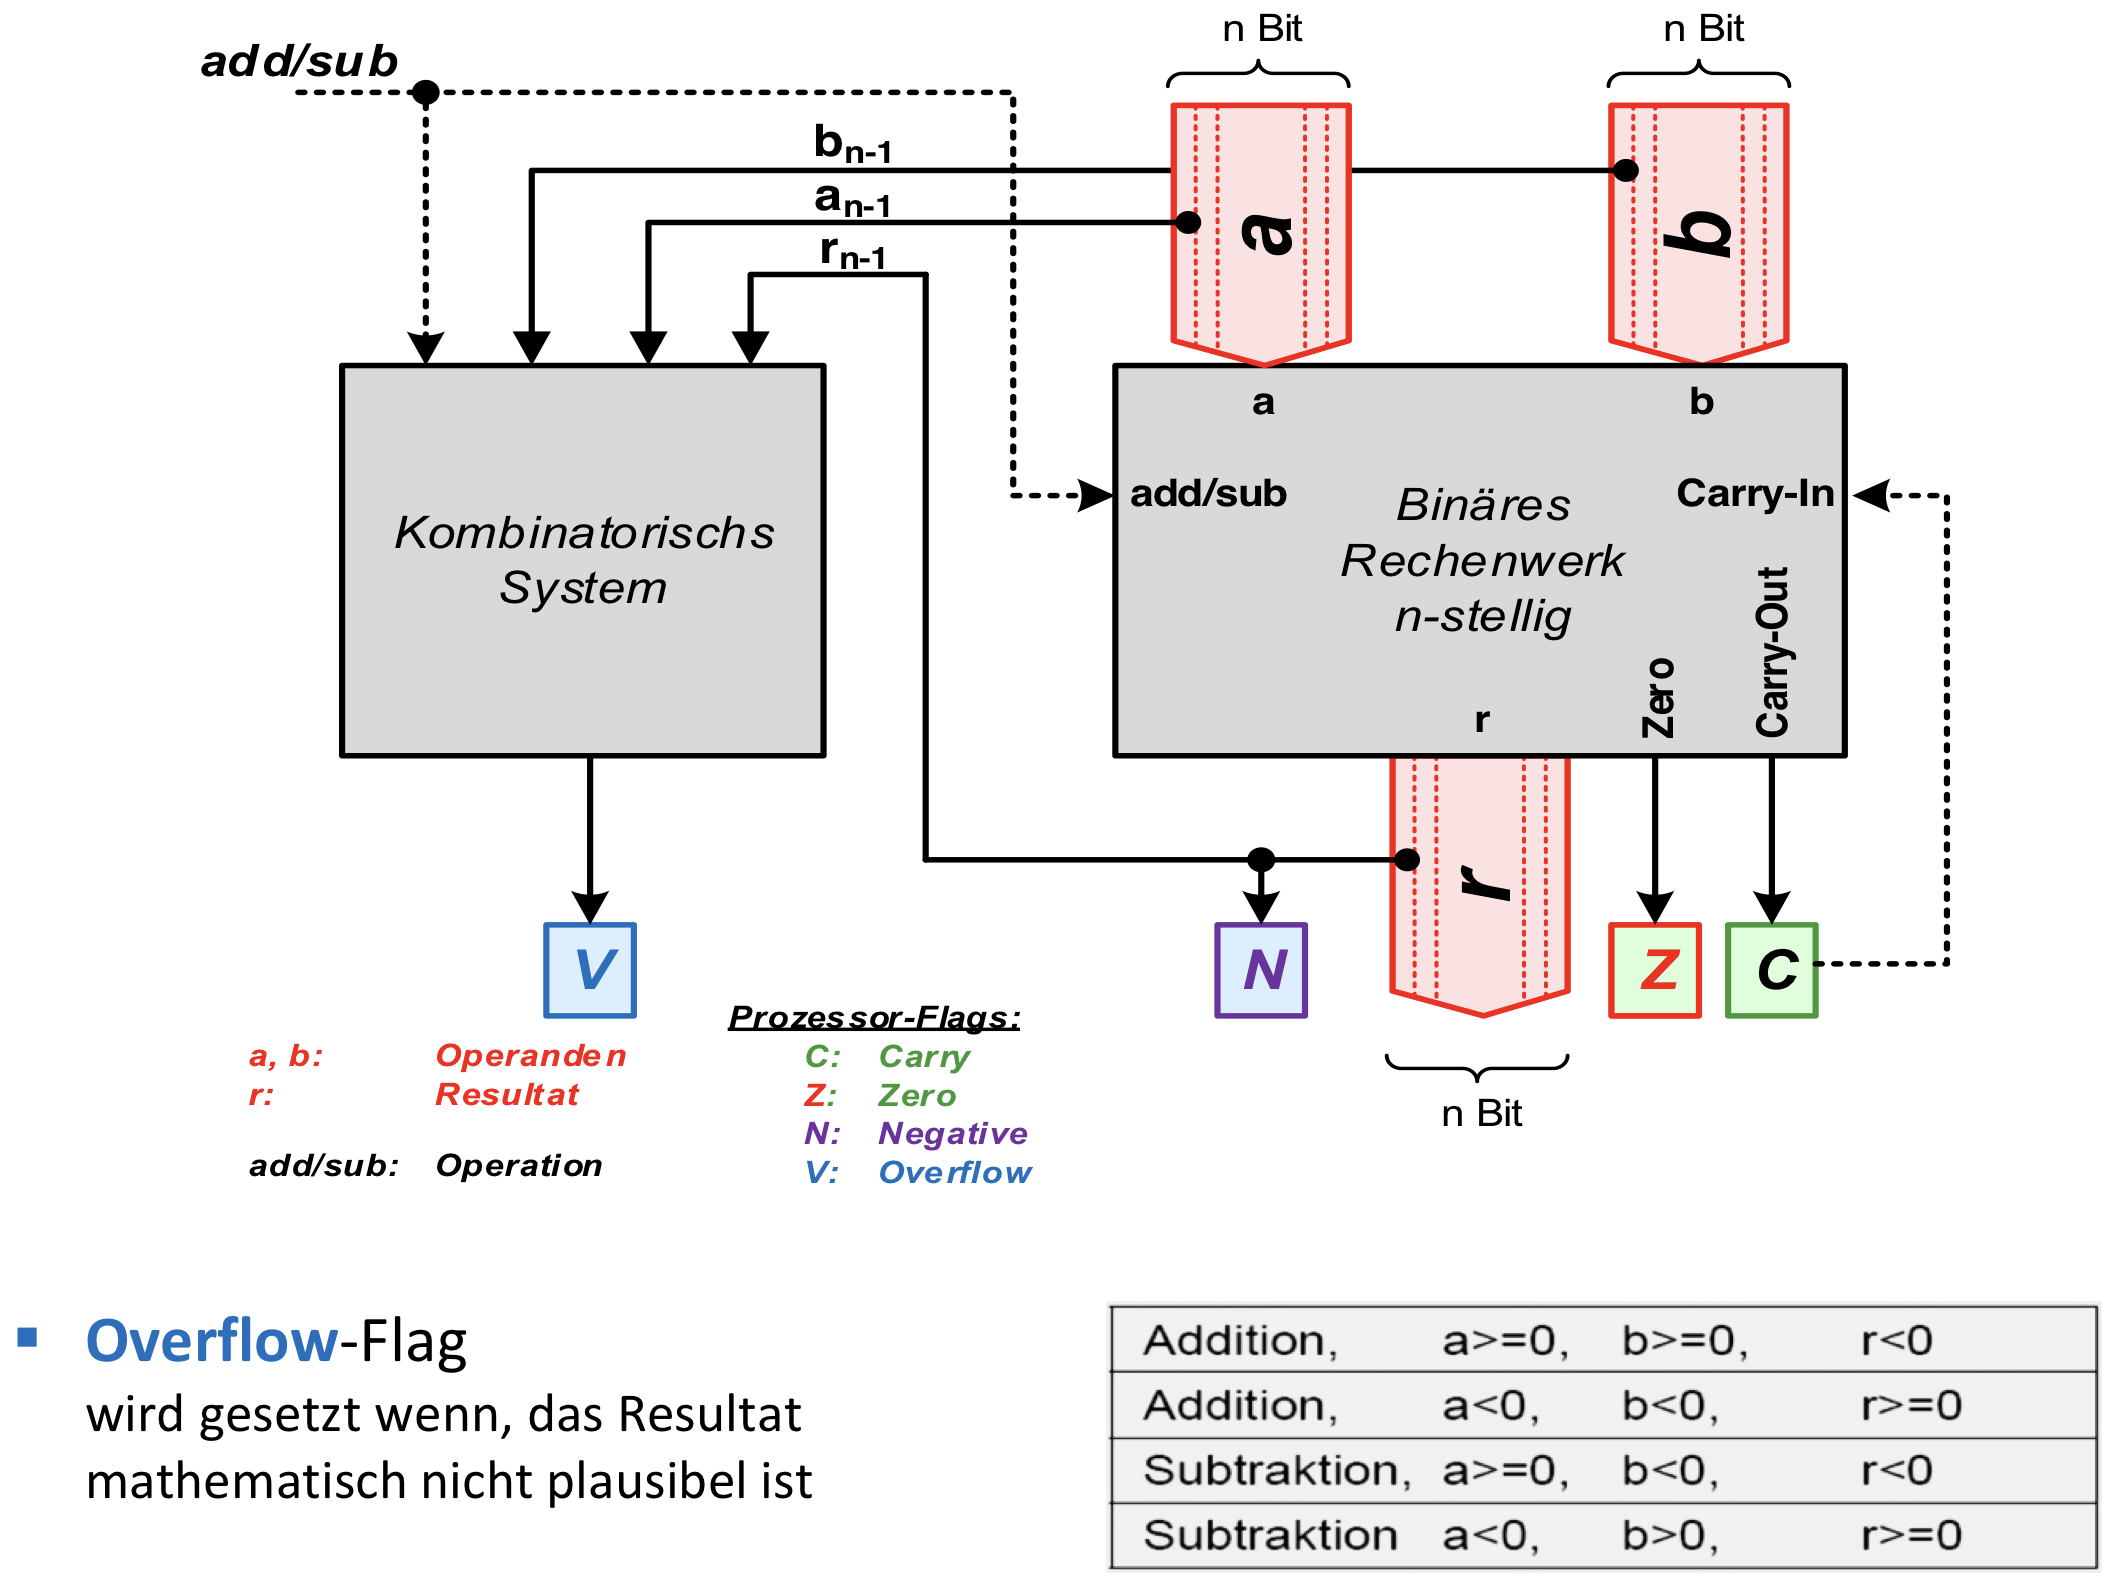
\includegraphics[width=8.5cm]{pics/Duales_rechenwerk}
	
	Das duale Rechenwerk f"uhrt nicht nur Addition und Subtraktion zweier Zahlen durch sondern setzt zudem auch das Zero- und Carry-Flag. Das Overflow-Flag muss noch mit einem kombinatorischen System bestimmt werden.
\end{minipage}
%
\begin{minipage}{0.5cm}
	\ \
\end{minipage}
%
\begin{minipage}[t]{8cm}
	\vspace{-4ex}
	\subsubsection{Operationen im dualen Rechenwerk}
	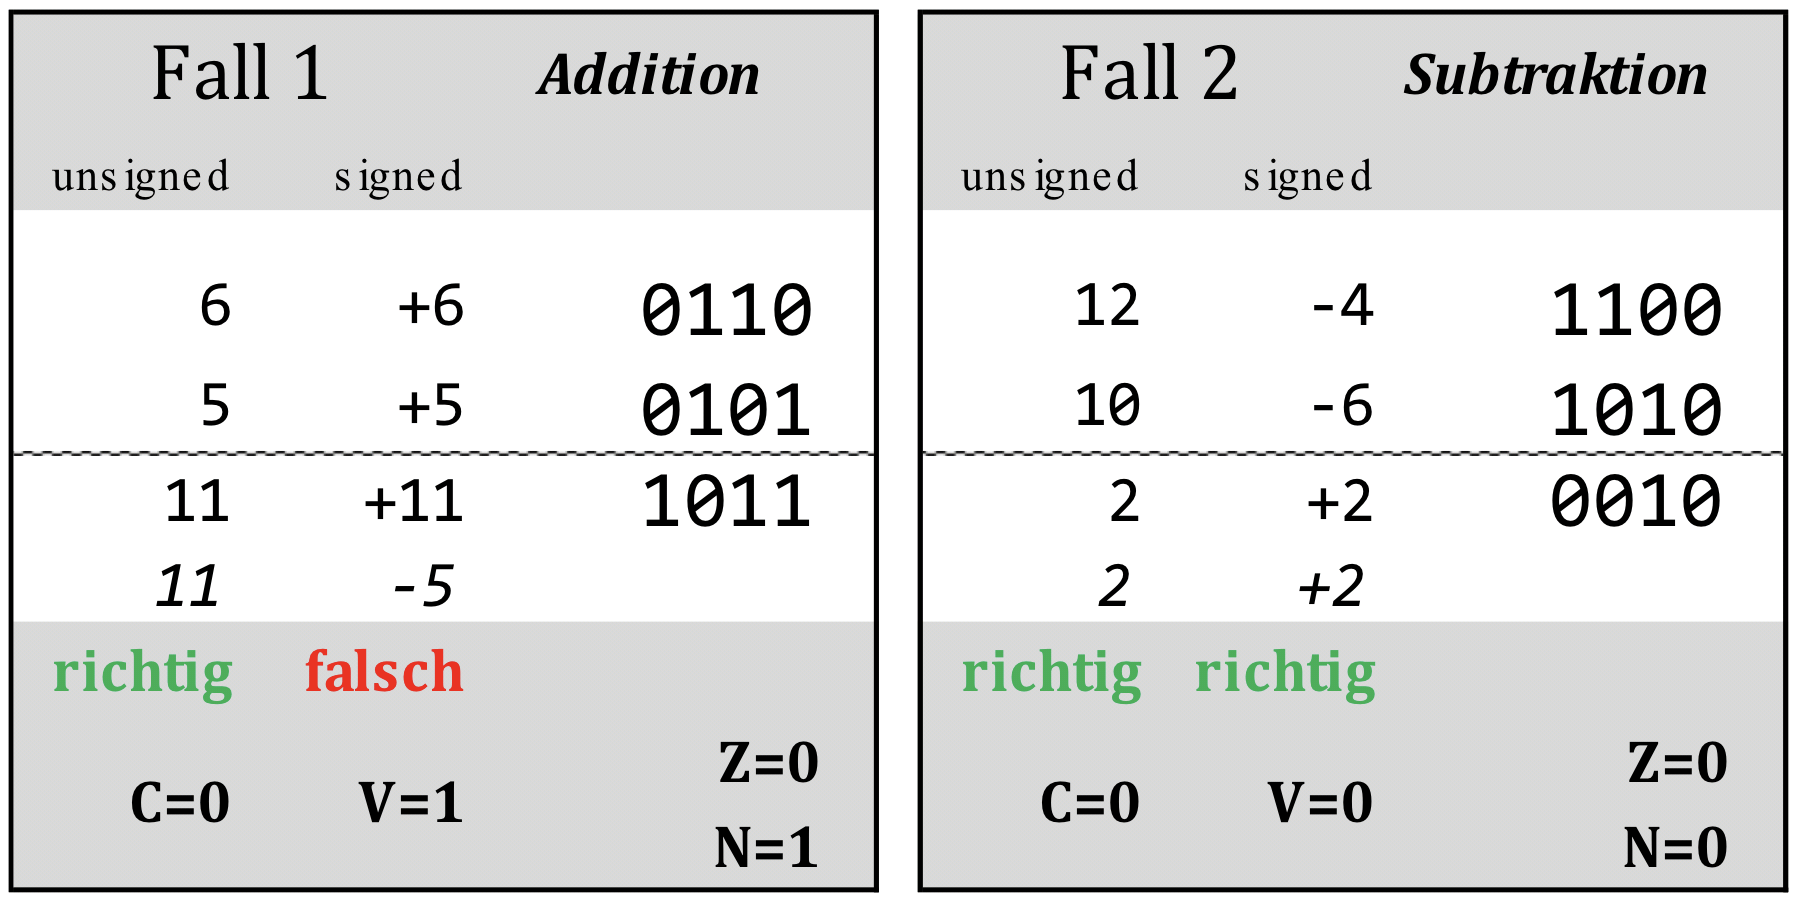
\includegraphics[width = 8cm]{pics/Bsp-Zahlenkreis-Zahlen}
	
	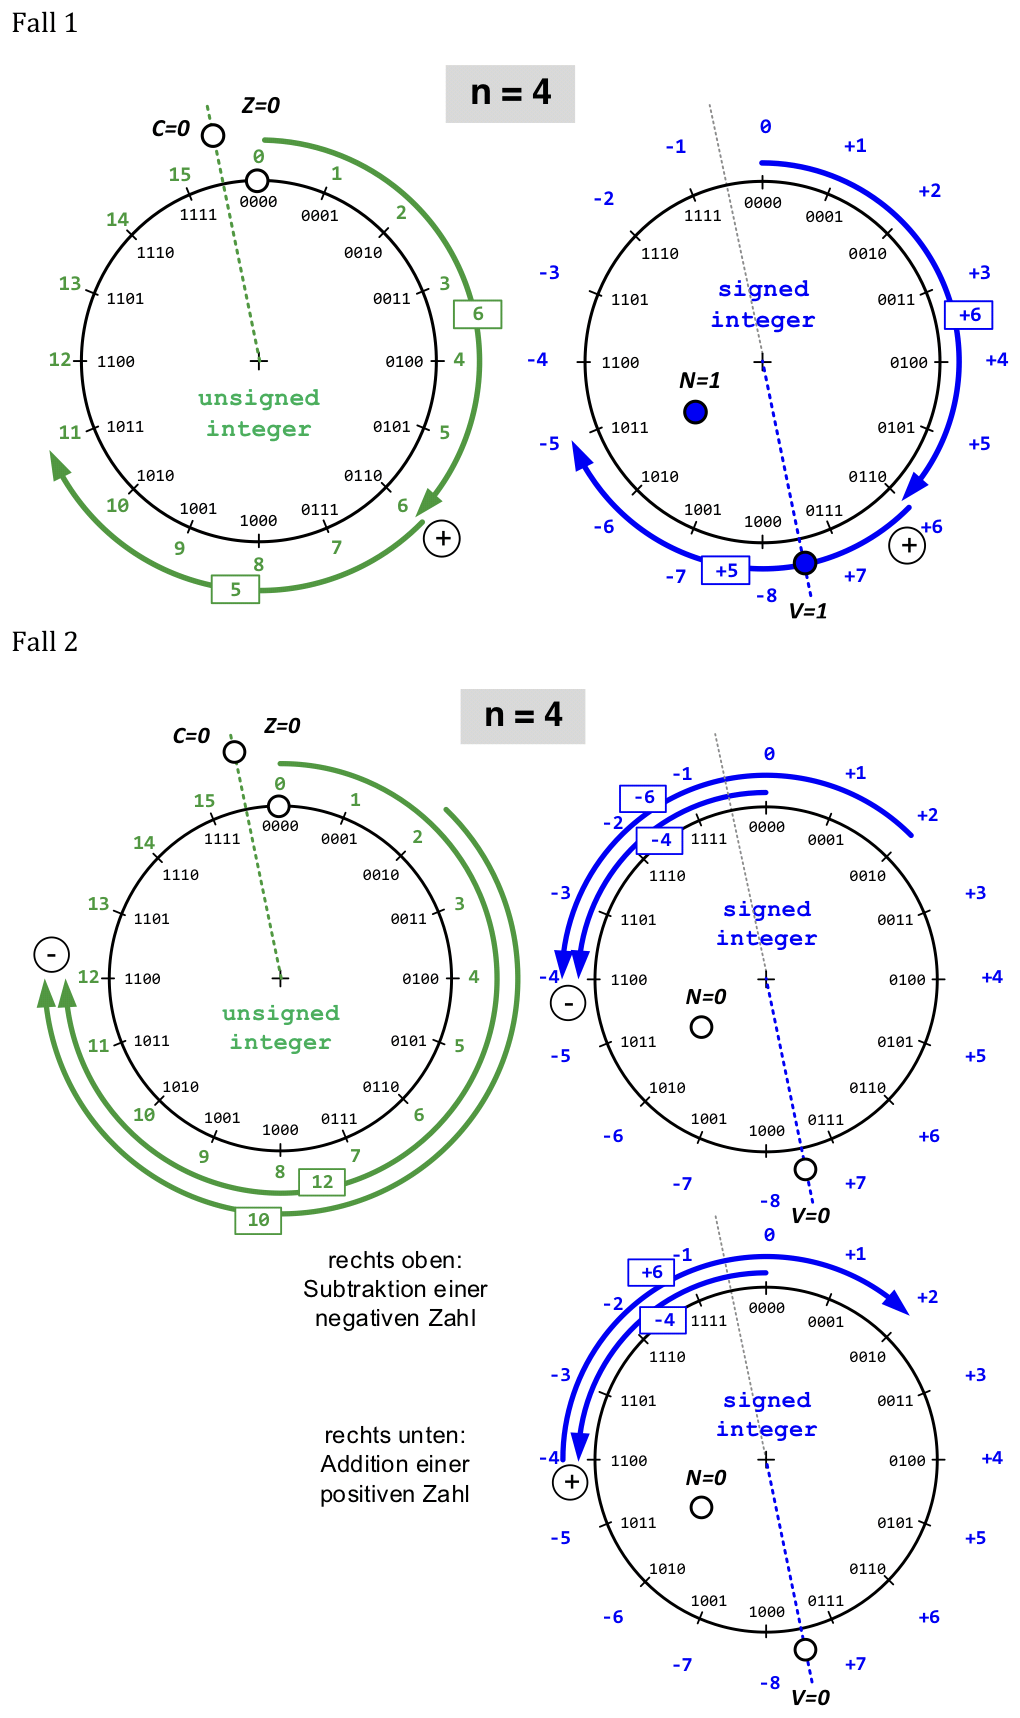
\includegraphics[width = 8cm]{pics/Bsp-Zahlenkreis}
	\begin{tabbing}
		\textbf{Al}\= \textbf{lgemeine Zahlenkreis Regeln}\\
		\> Addition: Zahlenvektoren hintereinander reihen\\
		\> Subtraktion: Zahlenvektoren stumpf gegeneinander\\
		\> stellen\\

		\textbf{signed integer}\\
		\> Flags: Negative, Overflow, Zero\\
		\> positiv: Zahlenvektoren Uhrzeigersinn\\
		\> negativ: Zahlenvektoren Gegenuhrzeigersinn\\
	
		\textbf{unsigned integer}\\
		\> Flags: Zero, Carry\\
		\> Zahlenvektoren immer Uhrzeigersinn\\
	\end{tabbing}
\end{minipage}

\subsection{Alternative Darstellungen von vorzeichenbehafteten Ganzzahlen}
\subsubsection{Gr"ossendarstellung mit Vorzeichen (signed magnitude)}
\vspace{-2ex}
\begin{minipage}{9cm}
	\begin{tabbing}
		MS\=B gibt  Vorzeichen an:\\
		\> $d_{n-1} = 0 \Rightarrow$ positive Zahl\\
		\> $d_{n-1} = 1 \Rightarrow$ negative Zahl\\\\
		
		Bemerkungen, Probleme:\\
		\> Es entstehen zwei verschiedene Darstellungen der Null\\
		\> z.B. bei n = 8: \= +0 \= = \%00000000\\
						\> \> -0 \> = \%10000000
		
	\end{tabbing}
\end{minipage}
%
\begin{minipage}{0.5cm}
	\ \
\end{minipage}
%
\begin{minipage}{9cm}
	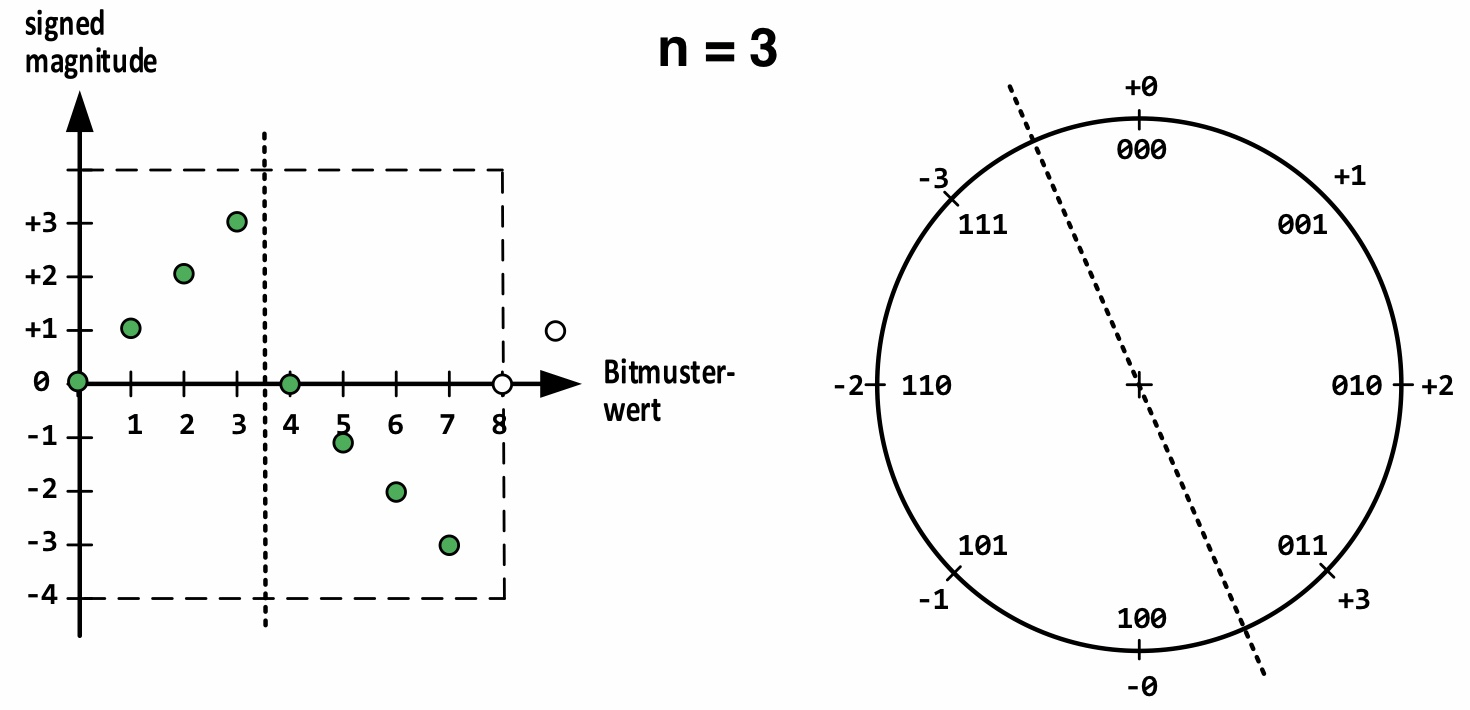
\includegraphics[width=8cm]{pics/Signed_Magnitude}
\end{minipage}

\subsubsection{Einerkomplement}
\vspace{-2ex}
\begin{minipage}{9cm}
	\begin{tabbing}
		MS\=B gibt  Vorzeichen an:\\
		\> $d_{n-1} = 0 \Rightarrow$ positive Zahl\\
		\> $d_{n-1} = 1 \Rightarrow$ negative Zahl\\\\
		
		Bemerkungen, Probleme:\\
		\> Es entstehen zwei verschiedene Darstellungen der Null\\
		\> z.B. bei n = 8: \= +0 \= = \%00000000\\
						\> \> -0 \> = \%11111111
		
	\end{tabbing}
\end{minipage}
%
\begin{minipage}{0.5cm}
	\ \
\end{minipage}
%
\begin{minipage}{9cm}
	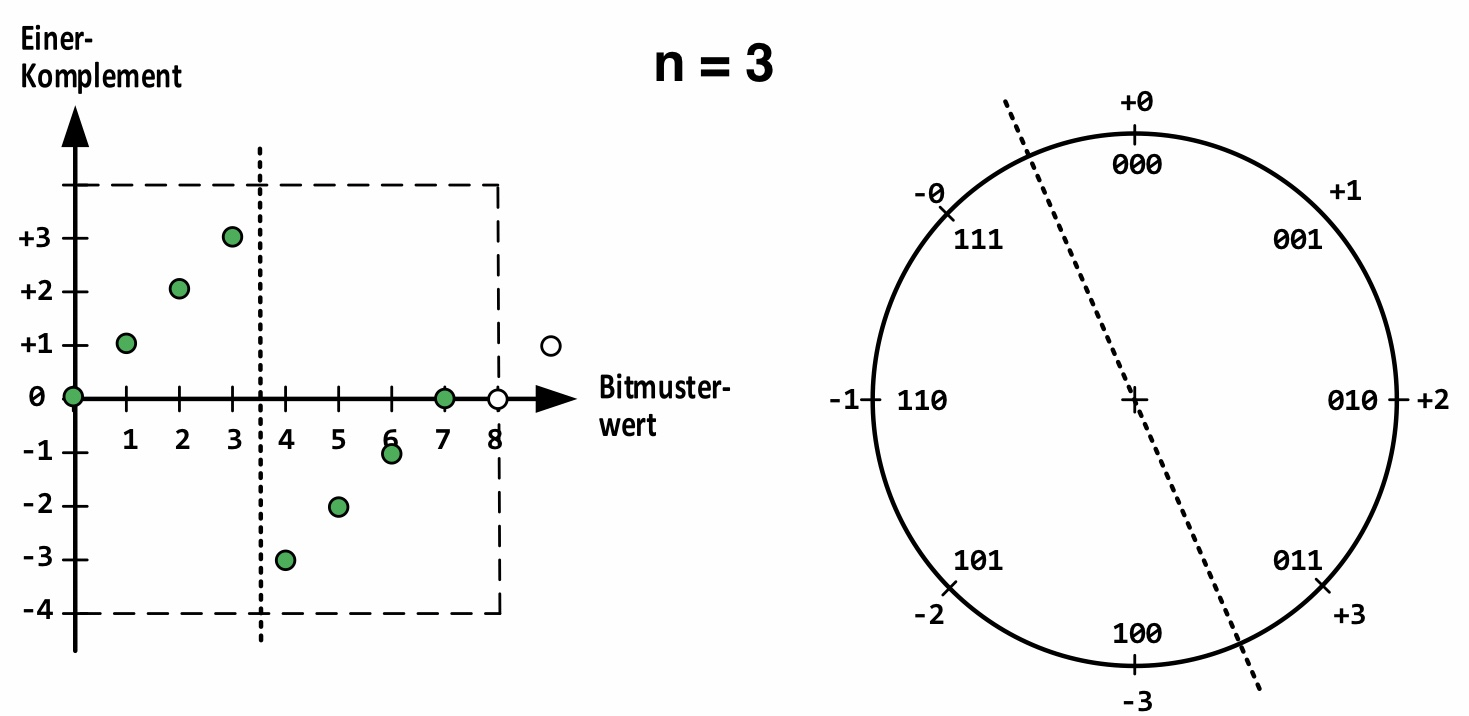
\includegraphics[width=8cm]{pics/Ones_Complement}
\end{minipage}

\subsubsection{Excess-Code, Stibitz-Code}
\begin{minipage}{9cm}
	\begin{tabbing}
		MS\=B gibt  Vorzeichen an:\\
		\> $d_{n-1} = 1 \Rightarrow$ positive Zahl\\
		\> $d_{n-1} = 0 \Rightarrow$ negative Zahl\\
		Wert = Bitmusterwert - $2^{n-1}$\\\\
		Bemerkungen, Probleme:\\
		\> Eindeutiges Bitmuster f"ur Null\\
		\> Zweierkomplement um den Exzess von $\mathbf{2^{n-1}}$ verschoben\\
		\> Excess-Code wird beispielsweise f"ur die Floating-Point \\
		\> Darstellung verwendet	
	\end{tabbing}
\end{minipage}
%
\begin{minipage}{0.5cm}
	\ \
\end{minipage}
%
\begin{minipage}{9cm}
	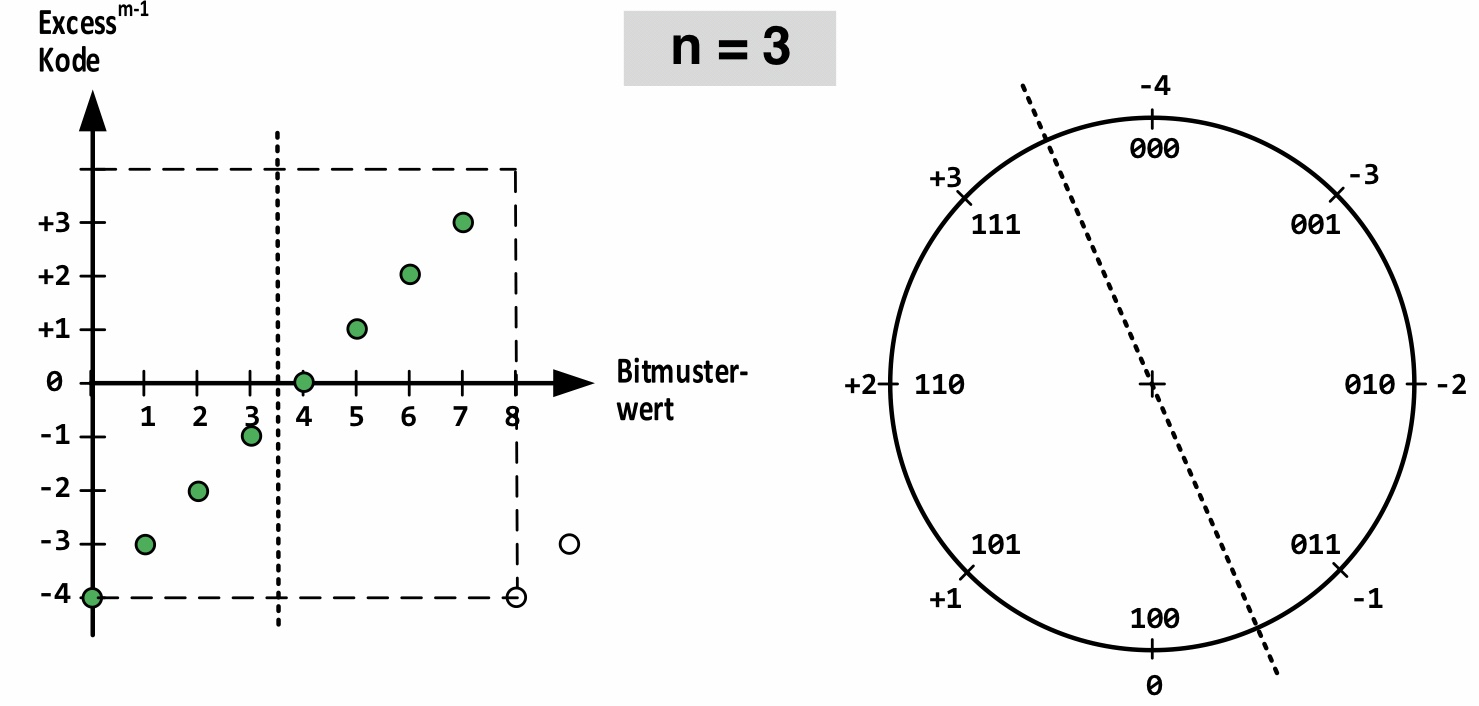
\includegraphics[width=8cm]{pics/Excess_Code}
\end{minipage}

\subsection{Festkommazahlen}
\begin{minipage}[t]{9cm}
	\subsubsection{IQ-Zahlen Format}
	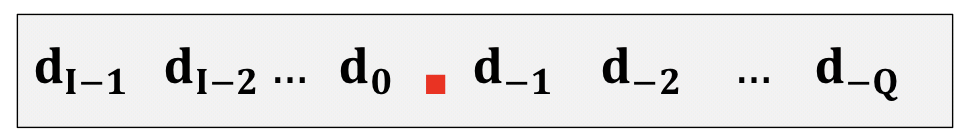
\includegraphics[width=5cm]{pics/IQ-Zahlen}
	\begin{itemize}
		\item \textbf{I}: Anzahl Integer-Stellen (Vorkommabitanzahl)
		\item \textbf{Q}: Anzahl Quotient-Stellen (Nachkommabitanzahl)
		\item Optimales Verh"altnis zwischen der erforderlichen Genauigkeit und dem n"otigen Wertebereich der Zahlendarstellung.
		\item Trennpunkt ist nur unsere Interpretation, Festkomma-Rechner rechnen immer mit reinen Bin"arzahlen
		\item Multiplikation und Division mit 2 kann mit Neuinterpretation der Bitfolge erreicht werden. \\(z.B. /2: I3Q2 $\Rightarrow$ I2Q3)
		\item \begin{tabular}{|l|l|l|l|}
				\hline
				\rowcolor[HTML]{C0C0C0} 
				Format             & Bin"ar          & Dezimal                       & Genauigkeit                \\ \hline
				\rowcolor[HTML]{EFEFEF} 
				{\color[HTML]{000000} I1Q3} & {\color[HTML]{000000} 1.000 ... 0.111} & {\color[HTML]{000000} -1 ... +7/8}  & {\color[HTML]{000000} 1/8} \\ \hline
				\rowcolor[HTML]{EFEFEF} 
				{\color[HTML]{000000} I2Q2} & {\color[HTML]{000000} 10.00 ... 01.11} & 	{\color[HTML]{000000} -2 ... +1.75} & {\color[HTML]{000000} 1/4} \\ \hline
				\rowcolor[HTML]{EFEFEF} 
				{\color[HTML]{000000} I3Q1} & {\color[HTML]{000000} 100.0 ... 011.1} & {\color[HTML]{000000} -4 ... +3.5}  & {\color[HTML]{000000} 1/2} \\ \hline
				\rowcolor[HTML]{EFEFEF} 
				{\color[HTML]{000000} I4Q0} & {\color[HTML]{000000} 1000 ... 0111}   & {\color[HTML]{000000} -8 ... +7}    & {\color[HTML]{000000} 1}   \\ \hline
			\end{tabular}	
	\end{itemize}
\end{minipage}
%
\begin{minipage}{0.5cm}
	\ \
\end{minipage}
%
\begin{minipage}[t]{9cm}
	\subsubsection{Fraktionale Zahlen}
		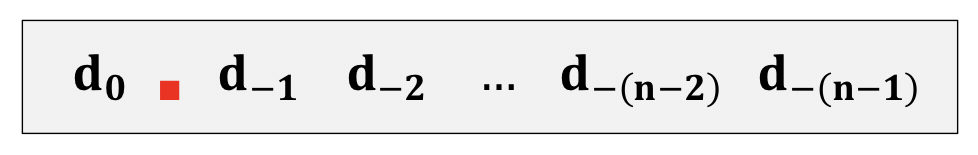
\includegraphics[width=5cm]{pics/Fraktionale_Zahlen}
		\begin{itemize}
			\item $\mathbf{d_0}$ gibt das Vorzeichen an
			\item Der Wertebereich ist immer: \color{blue} $\mathbf{-1.0 \leq W < +1.0}$ \color{black}
			\item Die Genauigkeit h"angt von der Bitanzahl \textbf{n} ab 
				\\$\Rightarrow$ \color{blue} $\mathbf{2^{-(n-1)}}$ \color{black}
			\item Wird h"aufig als Relativzahl oder Per-Unit-Zahl (PU) bezeichnet, da man den Wert prozentual zwischen $-100\%$ und $<+100\%$ auffassen kann.
			\item \begin{tabular}{|l|l|l|}
					\hline
					\rowcolor[HTML]{C0C0C0} 
					Bitanzahl & Dezimaler Wertebereich         & Schrittweite                  \\ \hline
					\rowcolor[HTML]{EFEFEF} 
					4         & $-1 \leq W <+1$ & $2^{-3}$     \\ \hline
					\rowcolor[HTML]{EFEFEF} 
					16        & $-1 \leq W <+1$ & $2^{-15}$    \\ \hline
					\rowcolor[HTML]{EFEFEF} 
					32        & $-1 \leq W <+1$ & $2^{-31}$ \\ \hline
					\rowcolor[HTML]{EFEFEF} 
					n         & $-1 \leq W <+1$ & $2^{-(n-1)}$ \\ \hline		
				\end{tabular}				
		\end{itemize}
\end{minipage}

\subsection{Gleitkommazahlen}
Da Festkommazahlen bei einem kleinen Zahlenwert einen gr"osseren relativen Fehler haben als bei grossen Zahlenwerten wurden Gleitkommazahlen eingef"uhrt. Generell besteht eine Gleitkommazahl aus \textbf{Vorzeichen}, \textbf{Mantisse} und \textbf{Exponent}.
	F"ur Mikroprozessoren wurde dies mit dem \textbf{IEEE 754} standardisiert.
	
\subsubsection{IEEE 754: Grundformat}
	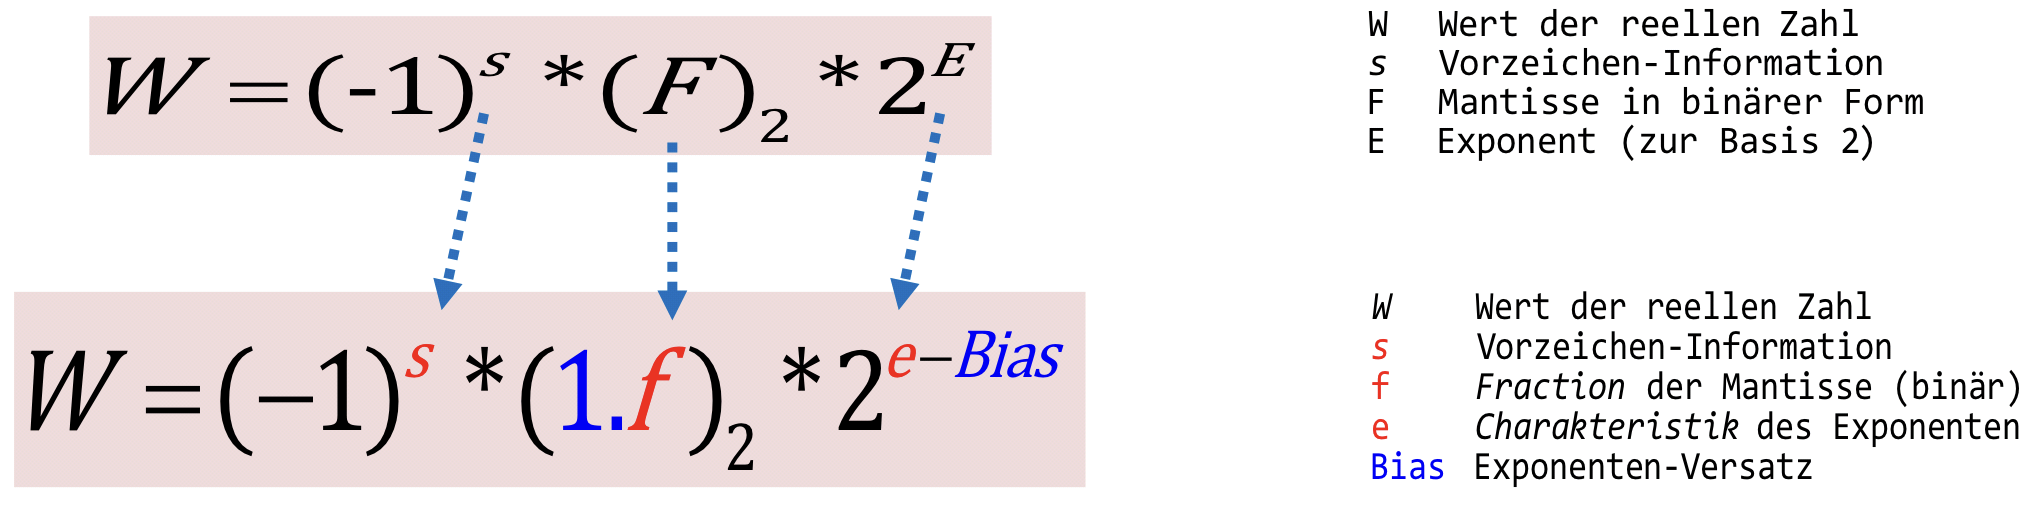
\includegraphics[width=12cm]{pics/IEEE-Grundformat_Darstellung}\\
	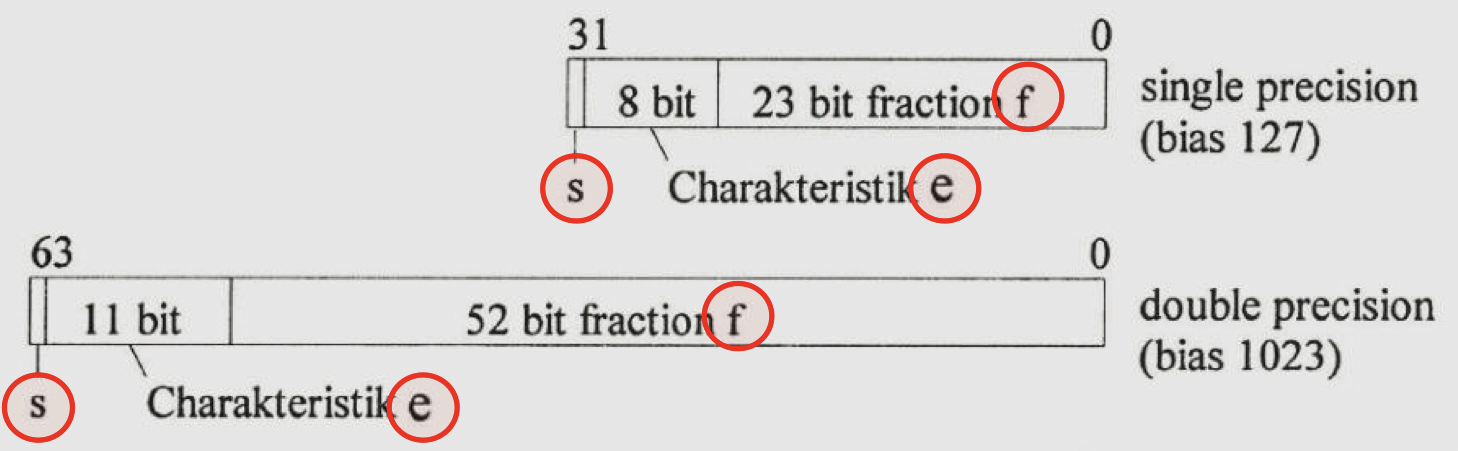
\includegraphics[width=9cm]{pics/IEEE-Grundformat}\\

\begin{minipage}[t]{9cm}
	\subsubsection{IEEE 754: Charakteristik}
	Die Exponenten-Information \color{red} \textbf{e} \color{black} wird auch als \textbf{Charakteristik} bezeichnet. Der transformierte Exponent \color{red} \textbf{e} \color{black} ergibt sich durch das Erh"ohen des Exponenten \textbf{E} um einen definierten \textbf{Bias} (Darstellung im \textbf{Excess-Code}).\\
	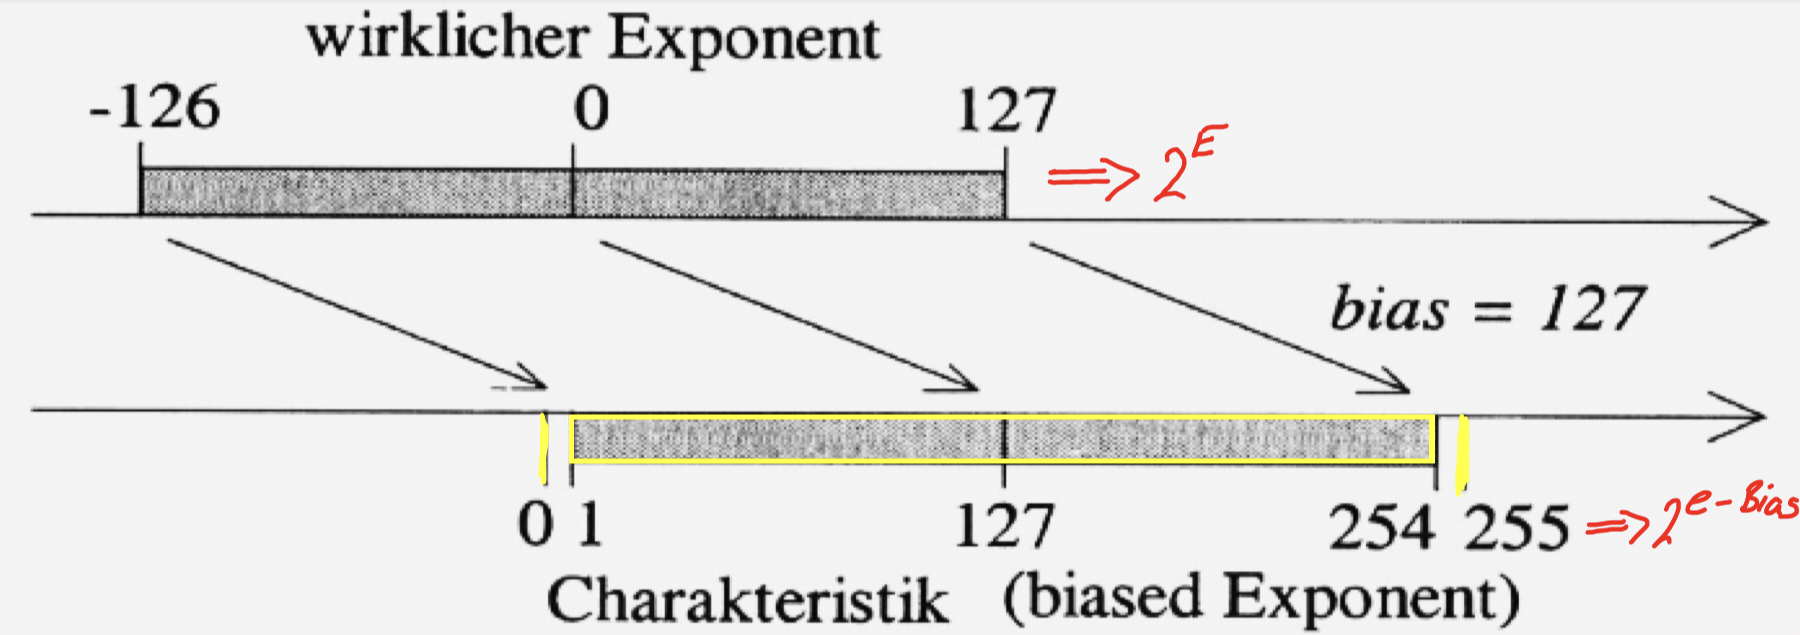
\includegraphics[width=7cm]{pics/IEEE-Exponent}
	\vspace{2ex}
	\subsubsection{Wertebereich und Kenngr"ossen}
	Kennwerte und Wertebereich f"ur die normalisierte Darstellung.\\
	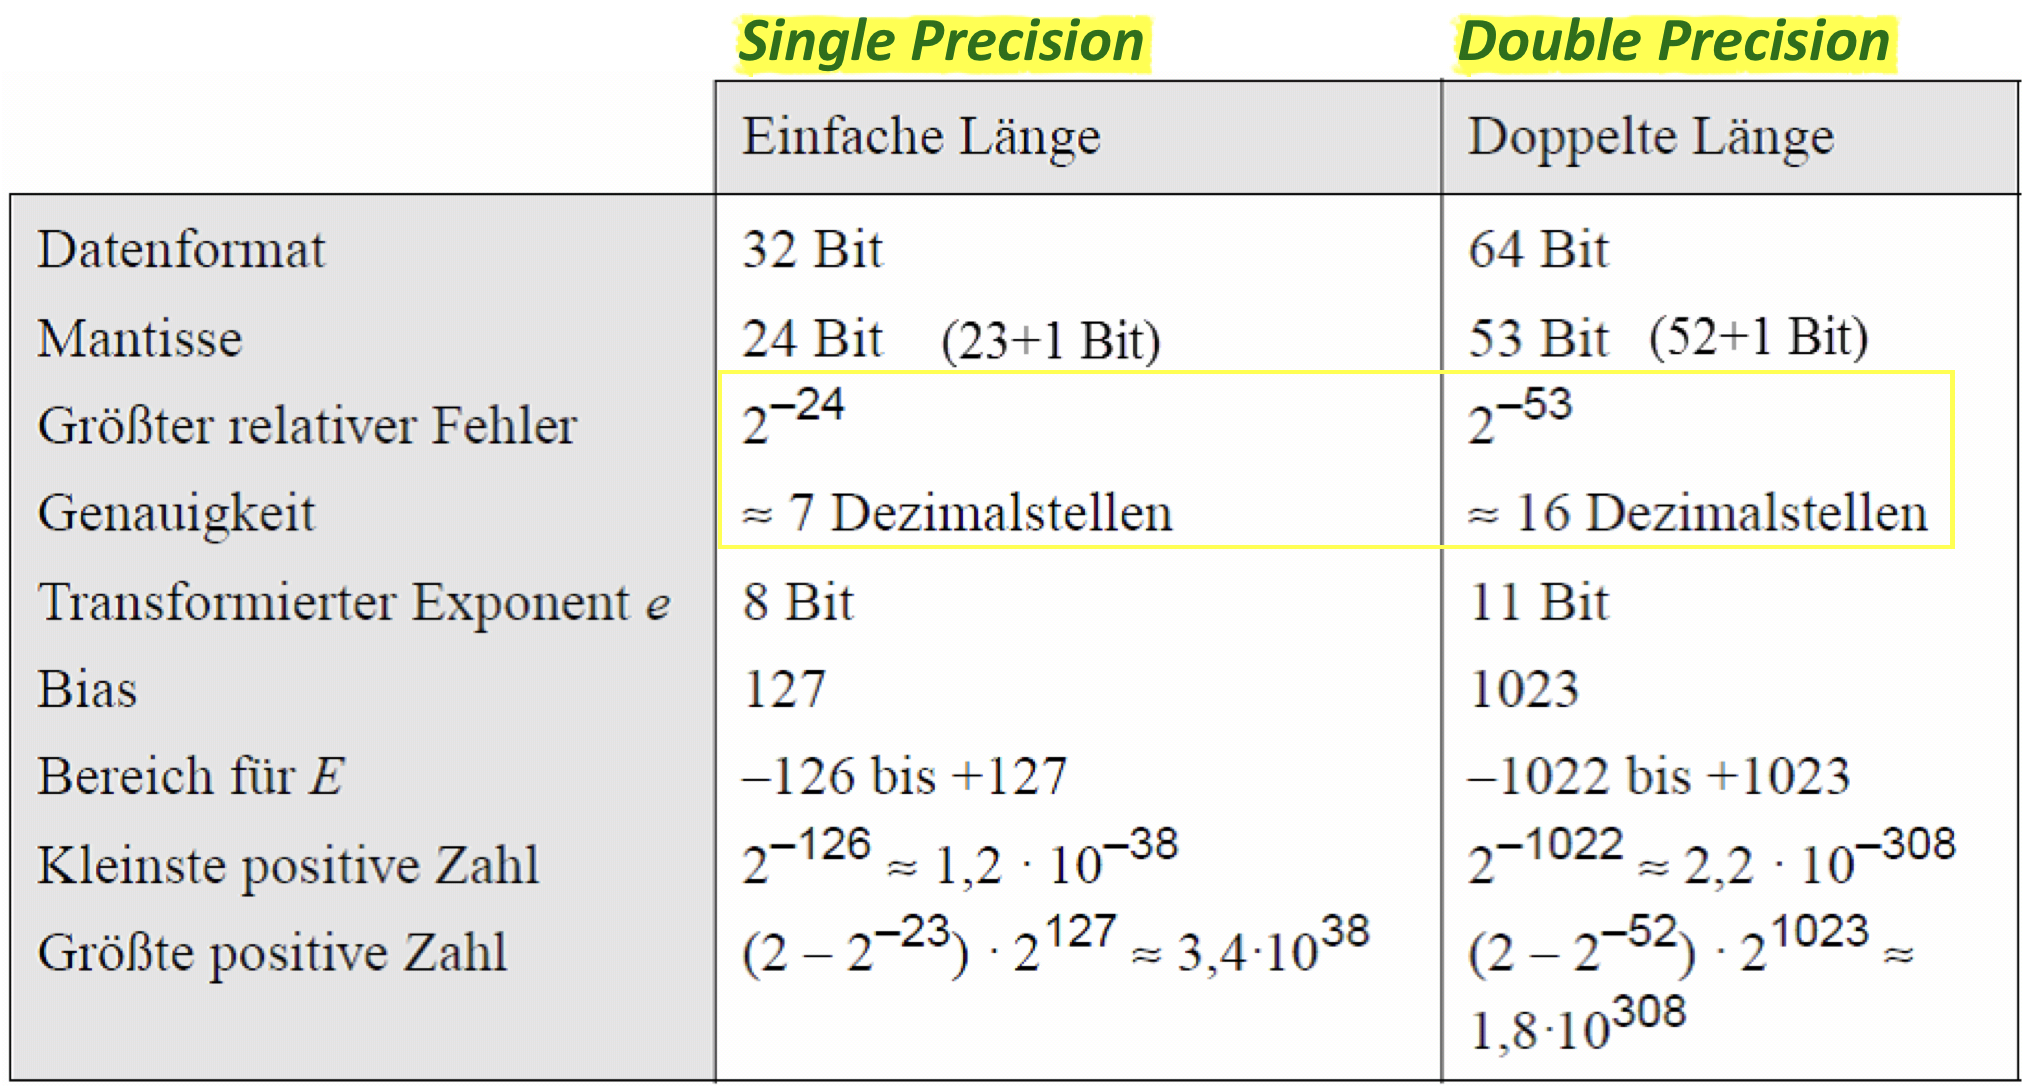
\includegraphics[width=8cm]{pics/IEEE-Wertbereich}
	\vspace{2ex}
	\subsubsection{IEEE 754: Berechnungsformeln}
		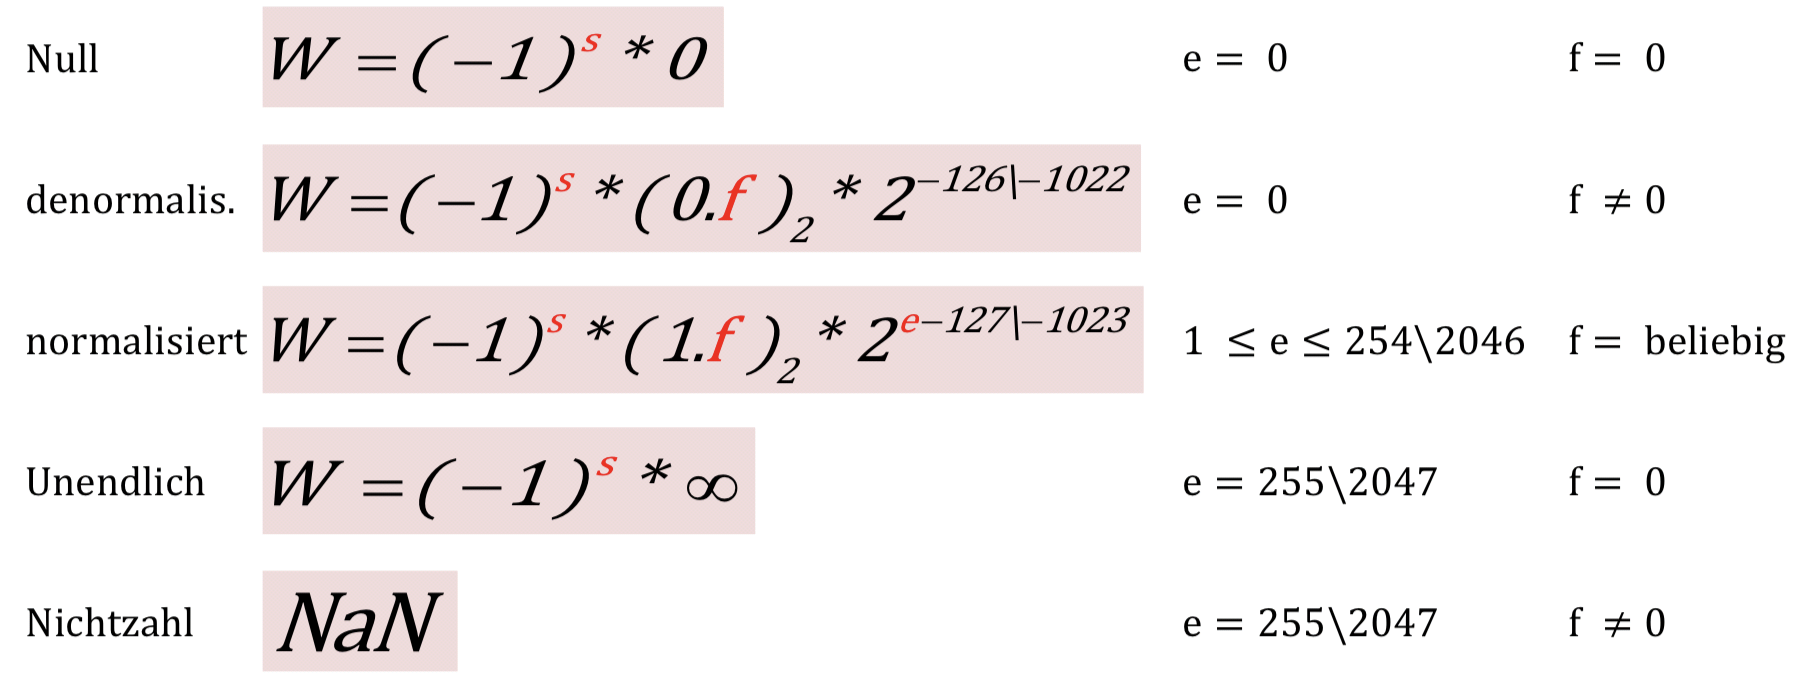
\includegraphics[width = 10cm]{pics/IEEE-Berechnungsformel}

\end{minipage}
%
\begin{minipage}{0.5cm}
	\ \
\end{minipage}
%
\begin{minipage}[t]{9cm}
			
	\subsubsection{Floating Point Operationen}
		\begin{tabbing}
			\textbf{Add}\=\textbf{ition, Subtraktion}\\
			\> Wenn die Exponenten ungleich sind muss der kleiner\\ 
			\> am gr"osseren angepasst werden. Dann werden die\\ 
			\> Mantissen addiert und wenn n"otig muss das Resultat\\ 
			\> noch normalisiert werden.\\
	
			\textbf{Multiplikation, Division}\\
			\> Bei der Multiplikation oder Division m"ussen die\\
			\> Exponenten addiert oder subtrahiert werden und die\\ 
			\> Mantissen mit der jeweiligen Operation verrechnet\\ 
			\> werden.
		\end{tabbing}

	\subsubsection{Zahlengerade f"ur Single Precision Numbers}
		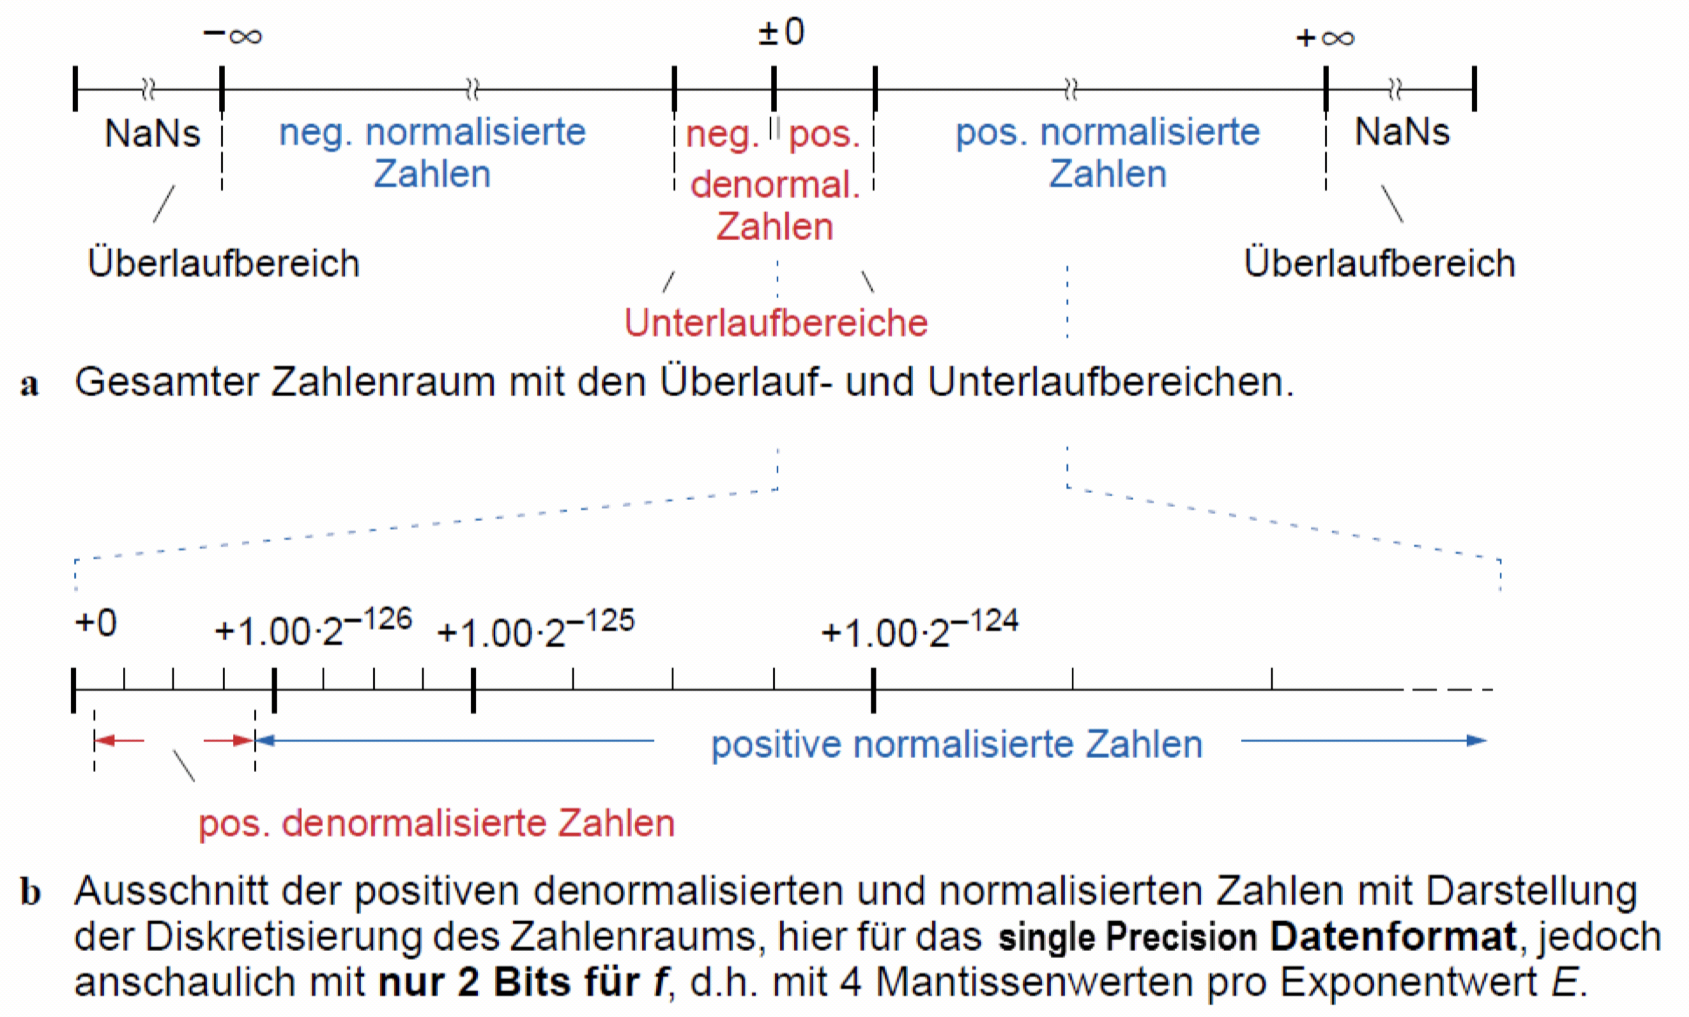
\includegraphics[width=9cm]{pics/IEEE-Zahlengerade}

\end{minipage}

\subsection{Zahlencodes}
Ein Code ist eine Vorschrift f"ur die eindeutige Zuordnung (Codierung) zweier Zeichenmengen (Urmenge, Bildmenge).
Folgende Numerische Codes sind von Bedeutung:
\begin{itemize}
	\item Zifferncodes: Jede Ziffer wird getrennt codiert, z.B. BCD.
	\item Positionscodes: Position des Bits innerhalb eines Wortes von Bedeutung
	\item Bewertbare Codes: Bitposition i hat definierte Wertigkeit, z.B. 8-4-2-1-Code
	\item Anordnungscodes: definiertes Bildungsgesetz, z.B. Excess-Code
	\item Einschrittige Codes: haben konstante Hamming-Distanz von 1
	\item Gleichgewichtete Codes (m-aus-n Codes): enthalten bei n Ziffernstellen m Einsen
	\item Fehlererkennungscodes: z.B. Dual-Code mit Parit"atsbit
	\item Fehlerkorrektur-Codes: erm"oglichen die Erkennung und die Korrektur falscher Bits
\end{itemize}

\subsubsection{BCD-Code}
\begin{minipage}{9cm}
\vspace{-8ex}
	Bei der BCD-Codierung (\textbf{Binary Coded Decimals}) werden die Ziffern der Dezimalzahl separat mit je vier Bit codiert. Der BCD-Code wird haupts"achlich verwendet um Rundungsfehler vermeiden zu k"onnen und Werte exakt darstellen zu k"onnen.\\
	Die sechs nicht verwendeten Bin"arwerte nennt man \textbf{Pseudotetraden}.
	\vspace{2ex}

	Beim Rechnen mit BCD-Zahlen muss auf Pseudotetraden geachtet werden, wenn solche entstehen m"ussen diese mit einer zus"atzlichen Addition von +6 korrigiert werden.
	\vspace{2ex}
	
	Beim Speichern von BCD-Zahlen gibt es das Packed- und Unpacked-BCD-Format. Beim \textbf{Unpacked BCD} wird jede BCD-Ziffern in der kleinsten adressierbaren Speichereinheit abgelegt. Beim \textbf{Packed BCD} werden mehrere BCD-Ziffern in eine Speichereinheit $"$gepackt$"$.
\end{minipage}
%
\begin{minipage}{0.5cm}
	\ \
\end{minipage}
%
\begin{minipage}{9cm}
	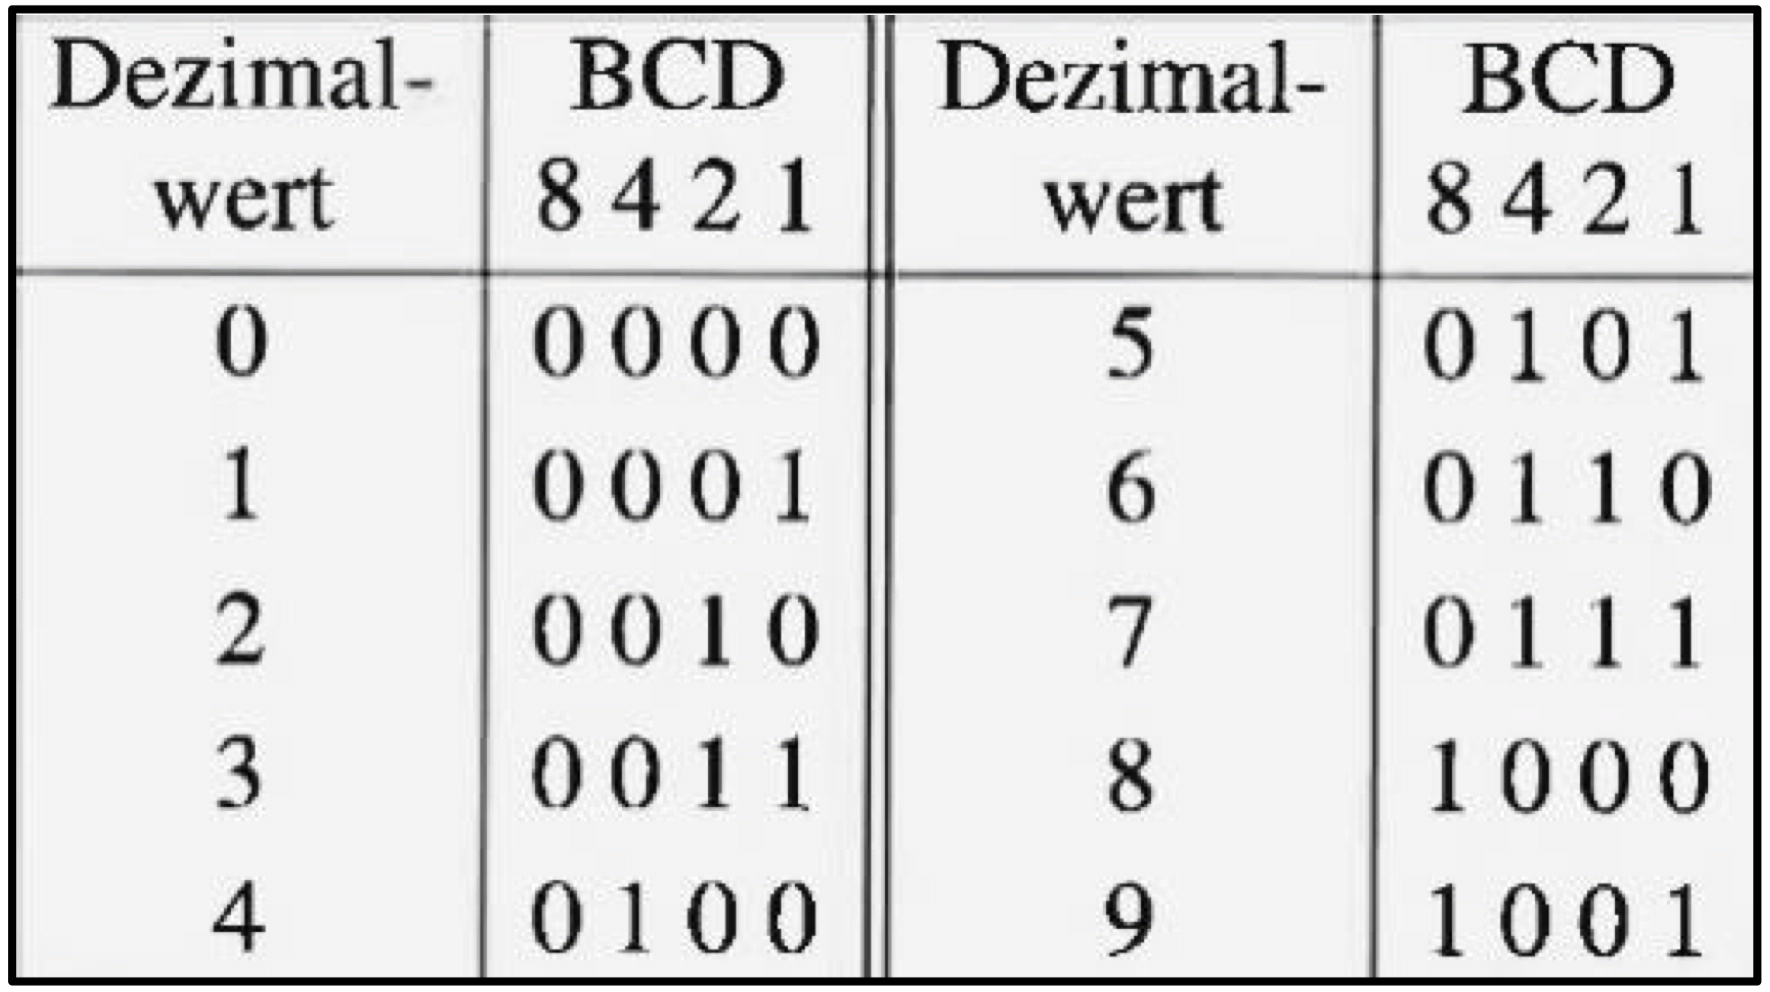
\includegraphics[width=4.5cm]{pics/2-BCD-Code}\\
	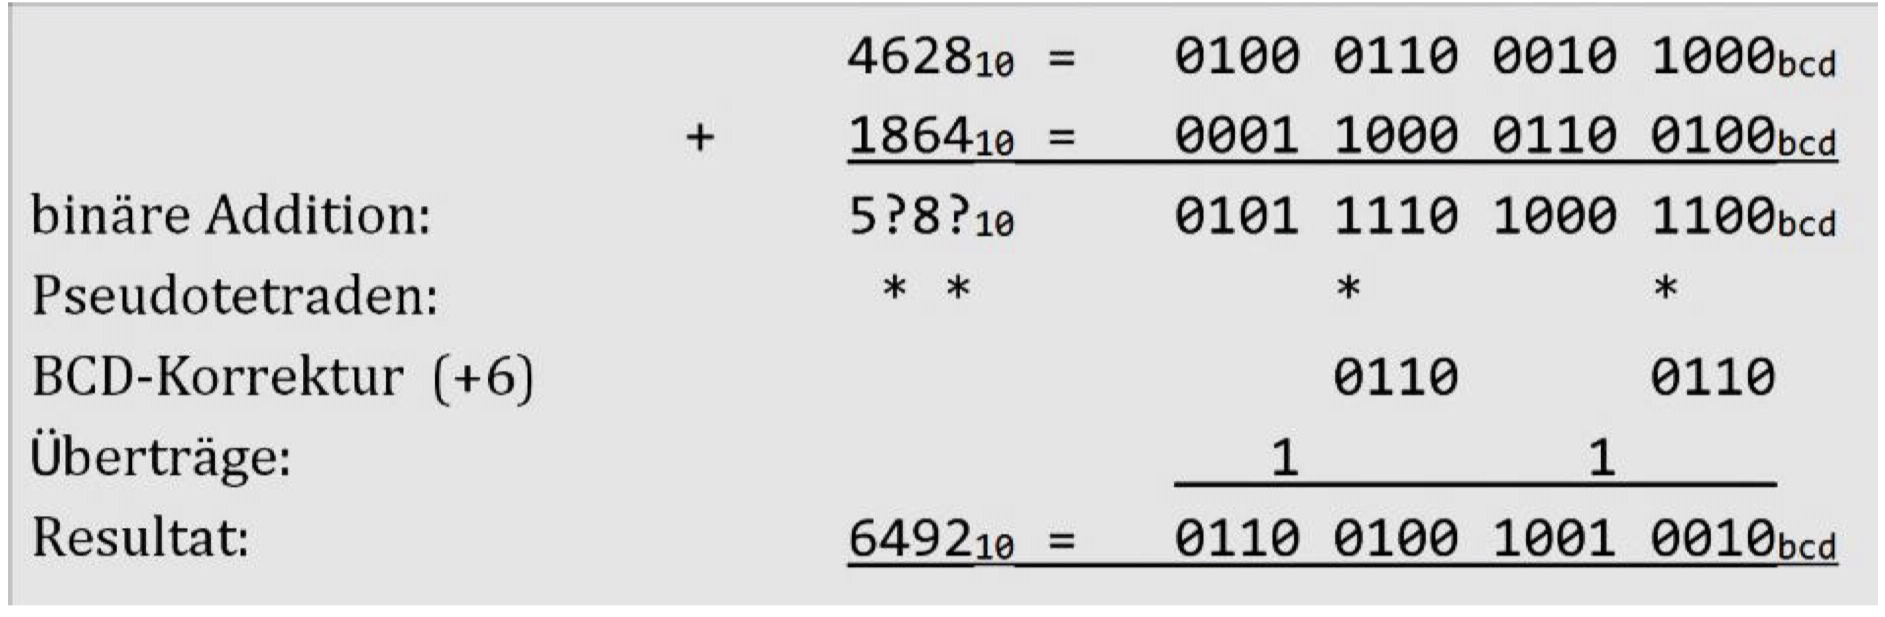
\includegraphics[width=8cm]{pics/2-Pseudo_Tetrade}\\
	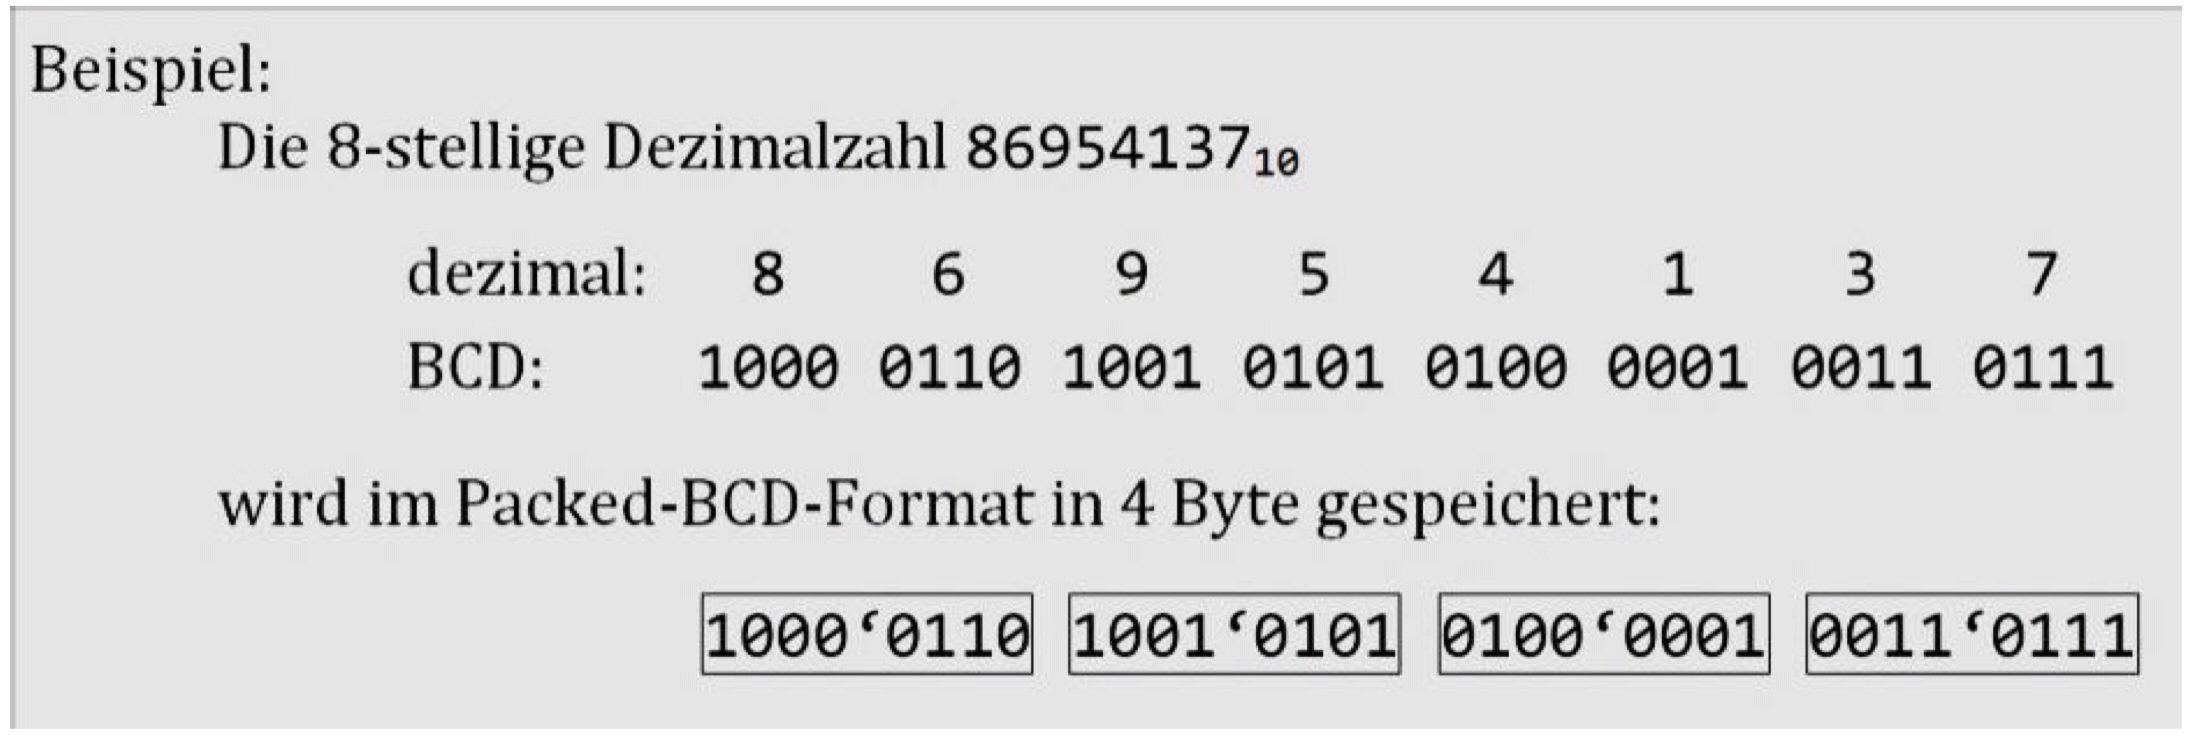
\includegraphics[width=8cm]{pics/2-Packed-BCD}
\end{minipage}

\subsubsection{Z"ahlcodes}
\begin{minipage}{9cm}
	\vspace{-6ex}
	Der Z"ahlcode kann sehr einfach codiert und decodiert werden und wird bei der Telefonimpulswahl verwendet: Die Einsen werden als Impulse umgesetzt, die Nullen als $"$keine Impulse$"$.
\end{minipage}
%
\begin{minipage}{0.5cm}
	\ \
\end{minipage}
%
\begin{minipage}{9cm}
	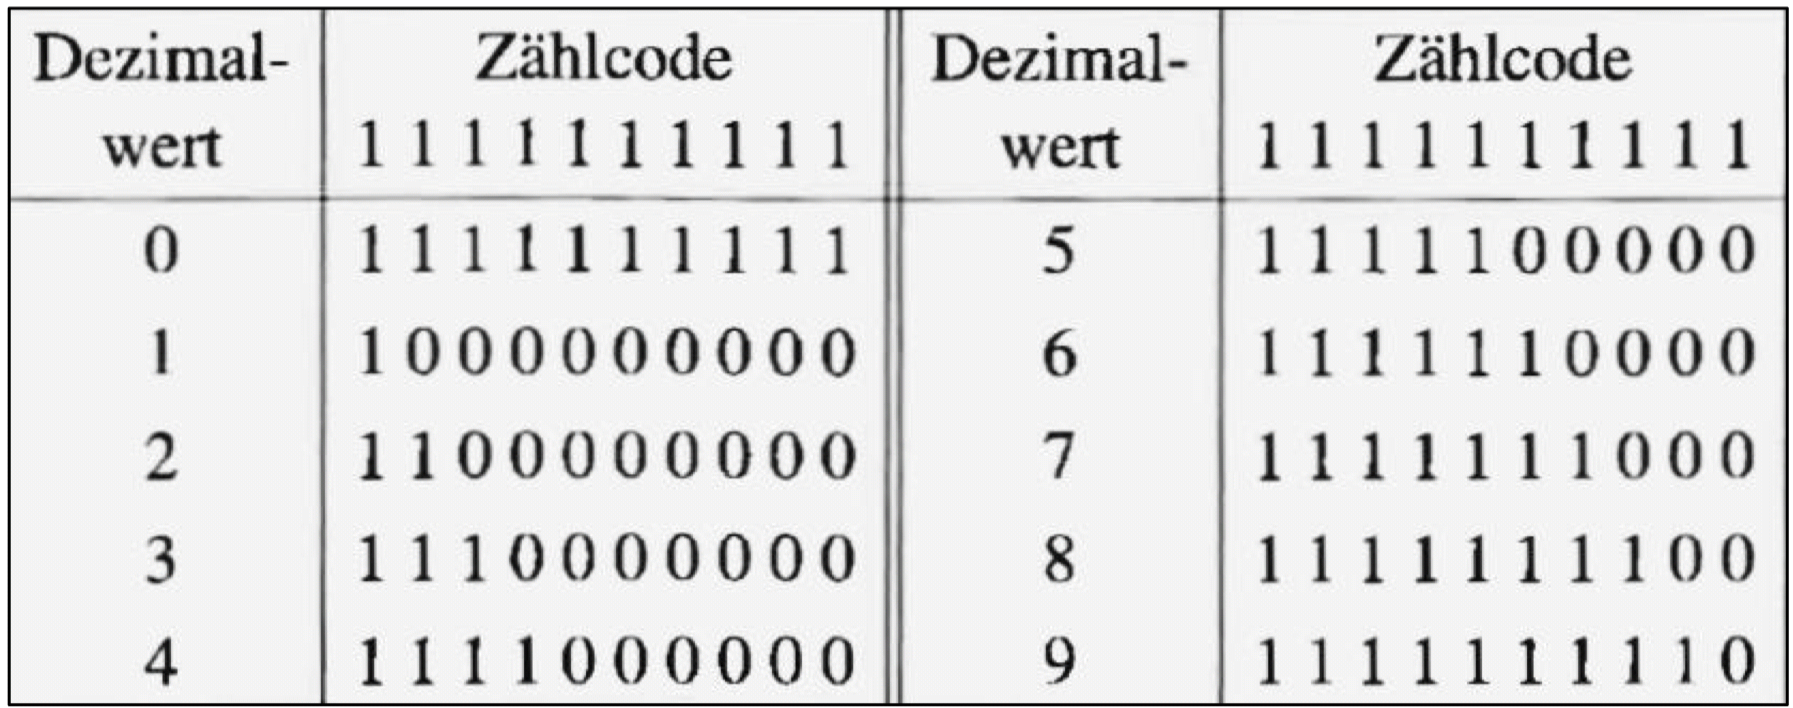
\includegraphics[width=6cm]{pics/2-Zaehlcodes}
\end{minipage}

\subsubsection{Codes mit Fehlererkennung}
Aus Gr"unden der Fehlererkennung werden oft \textbf{gleichgewichtete m-aus-n Codes} verwendet: z.B. in der Telekommunikation oder bei den Strichcodes.

\subsubsection{Gray-Code}
\begin{minipage}{9cm}
\vspace{-12ex}
	Der Gray-Code ist eine andere Darstellungsform des Bin"arcodes. Er hat die Eigenschaft, dass beim fortlaufenden Z"ahlen zwischen zwei benachbarten Codew"ortern immer nur ein Bit den Zustand wechselt (\textbf{einschrittiger Code}). Damit ergeben Ablesefehler im Zwischenbereich jeweils nur eine Unsicherheit von einem Bit, was gerade der Aufl"osegenauigkeit der gew"ahlten Codierung entspricht.
\end{minipage}
%
\begin{minipage}{0.5cm}
	\ \
\end{minipage}
%
\begin{minipage}{9cm}
	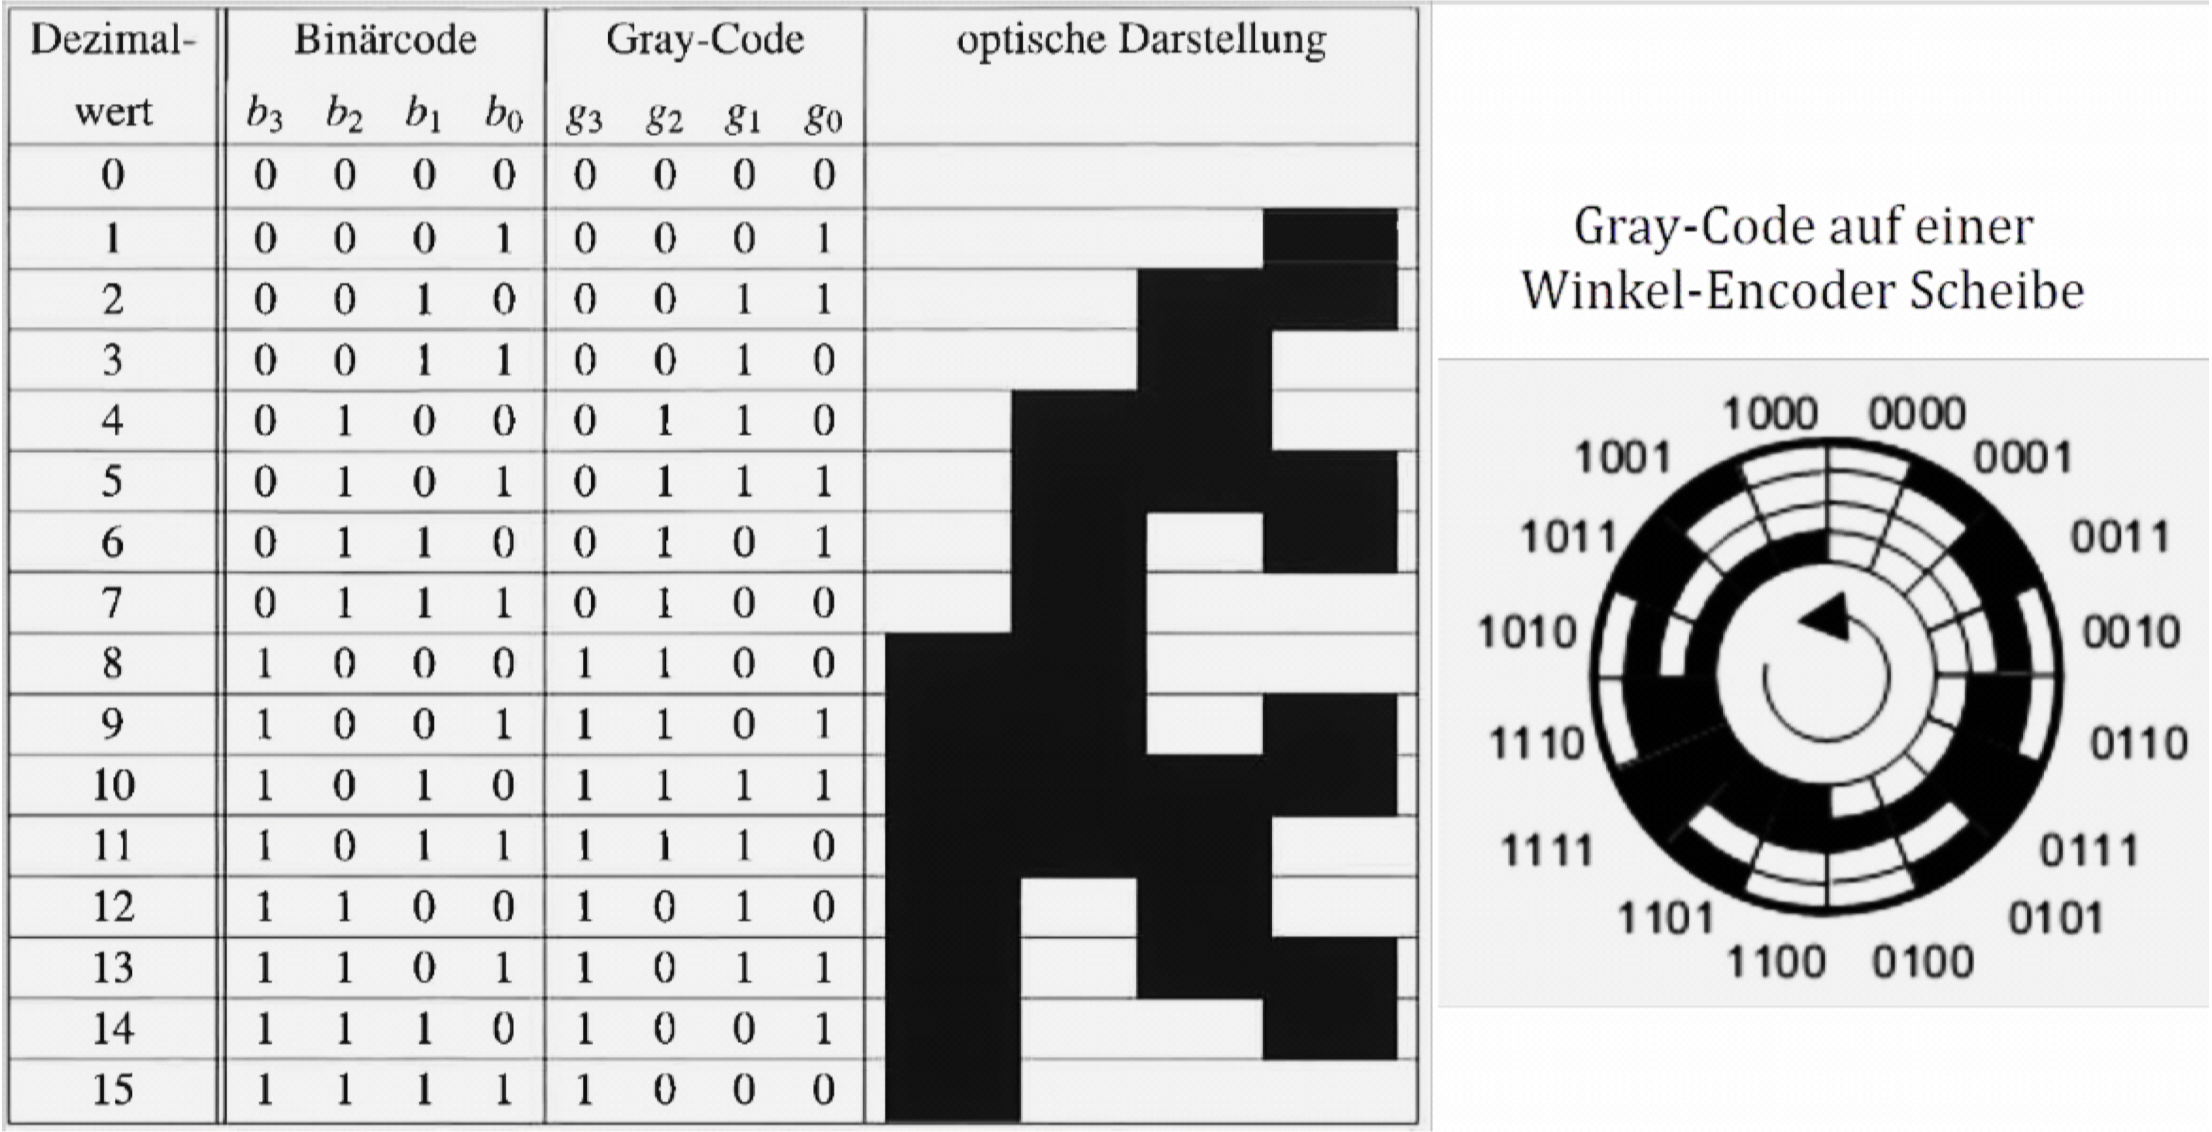
\includegraphics[width=9cm]{pics/2-Gray-Code}
\end{minipage}

\subsection{Zeichencodes}
\textbf{Alphanumerische Codes} dienen zur Darstellung von Ziffern, Buchstaben und  Sonderzeichen. Der am weitaus verbreiteste Zeichencode ist der \textbf{ASCII-Code}

\subsubsection{Unicode: universelle 16- und 32-Bit-Codes}
\begin{minipage}{9cm}
\vspace{-4ex}
	Der 16-Bit-Zeichencode UCS-2 wurde 1992 vom IEC genormt: Er enth"alt systematisch alle wichtigen nationalen und internationalen Zeichens"atze und den ASCII-Code als Untermenge am Anfang der Tabelle ab Index 0x0000.\\
	
	Dieser 16-Bit-Zeichencode ist wiederum eine Untermenge des 32-bit-Codes UCS-4, welcher Platz f"ur total 2 Milliarden Zeichen bietet.
\end{minipage}
%
\begin{minipage}{0.5cm}
	\ \
\end{minipage}
%
\begin{minipage}{9cm}
	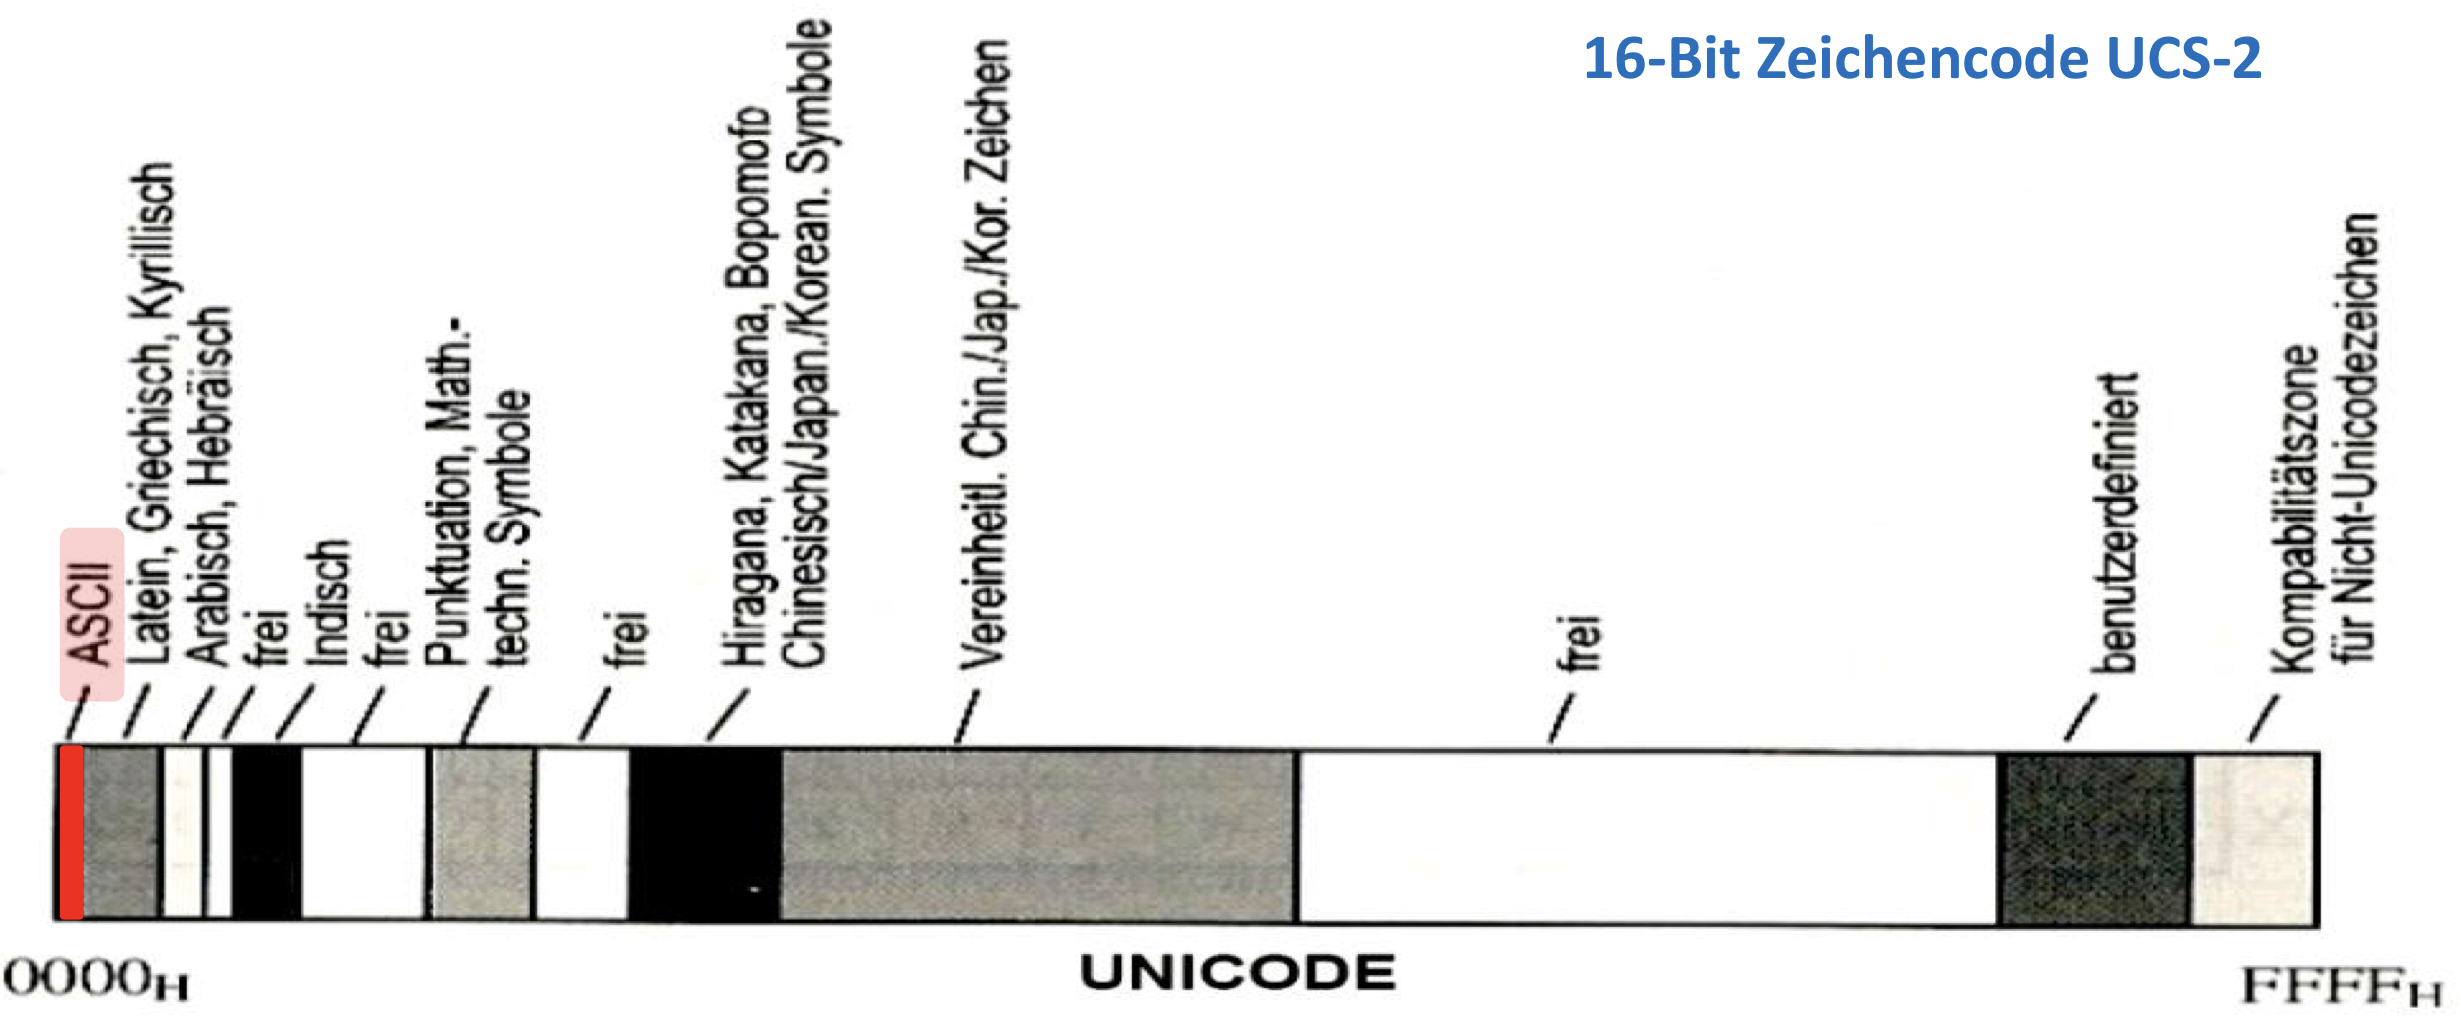
\includegraphics[width=9cm]{pics/2-Unicode}
\end{minipage}

\subsection{Fehlererkennung}
Aufgrund der Informationstheorie k"onnen Aussagen "uber die zus"atzlich notwendige Redundanz gemacht werden, um Ein- und Mehrbitfehler zu erkennen und allenfalls zu korrigieren.\\
Um eine Fehlererkennung durchf"uhren zu k"onnen ben"otigt es einen Codier-Mehraufwand (Redundanz). Solange alle Code-Kombinationen g"ultige Codeworte sind, wirkt sich jeder Fehler so aus, dass wiederum ein g"ultiges Codewort entsteht.

\vspace{2ex}
\begin{minipage}{9cm}
	\subsubsection{Definition}
		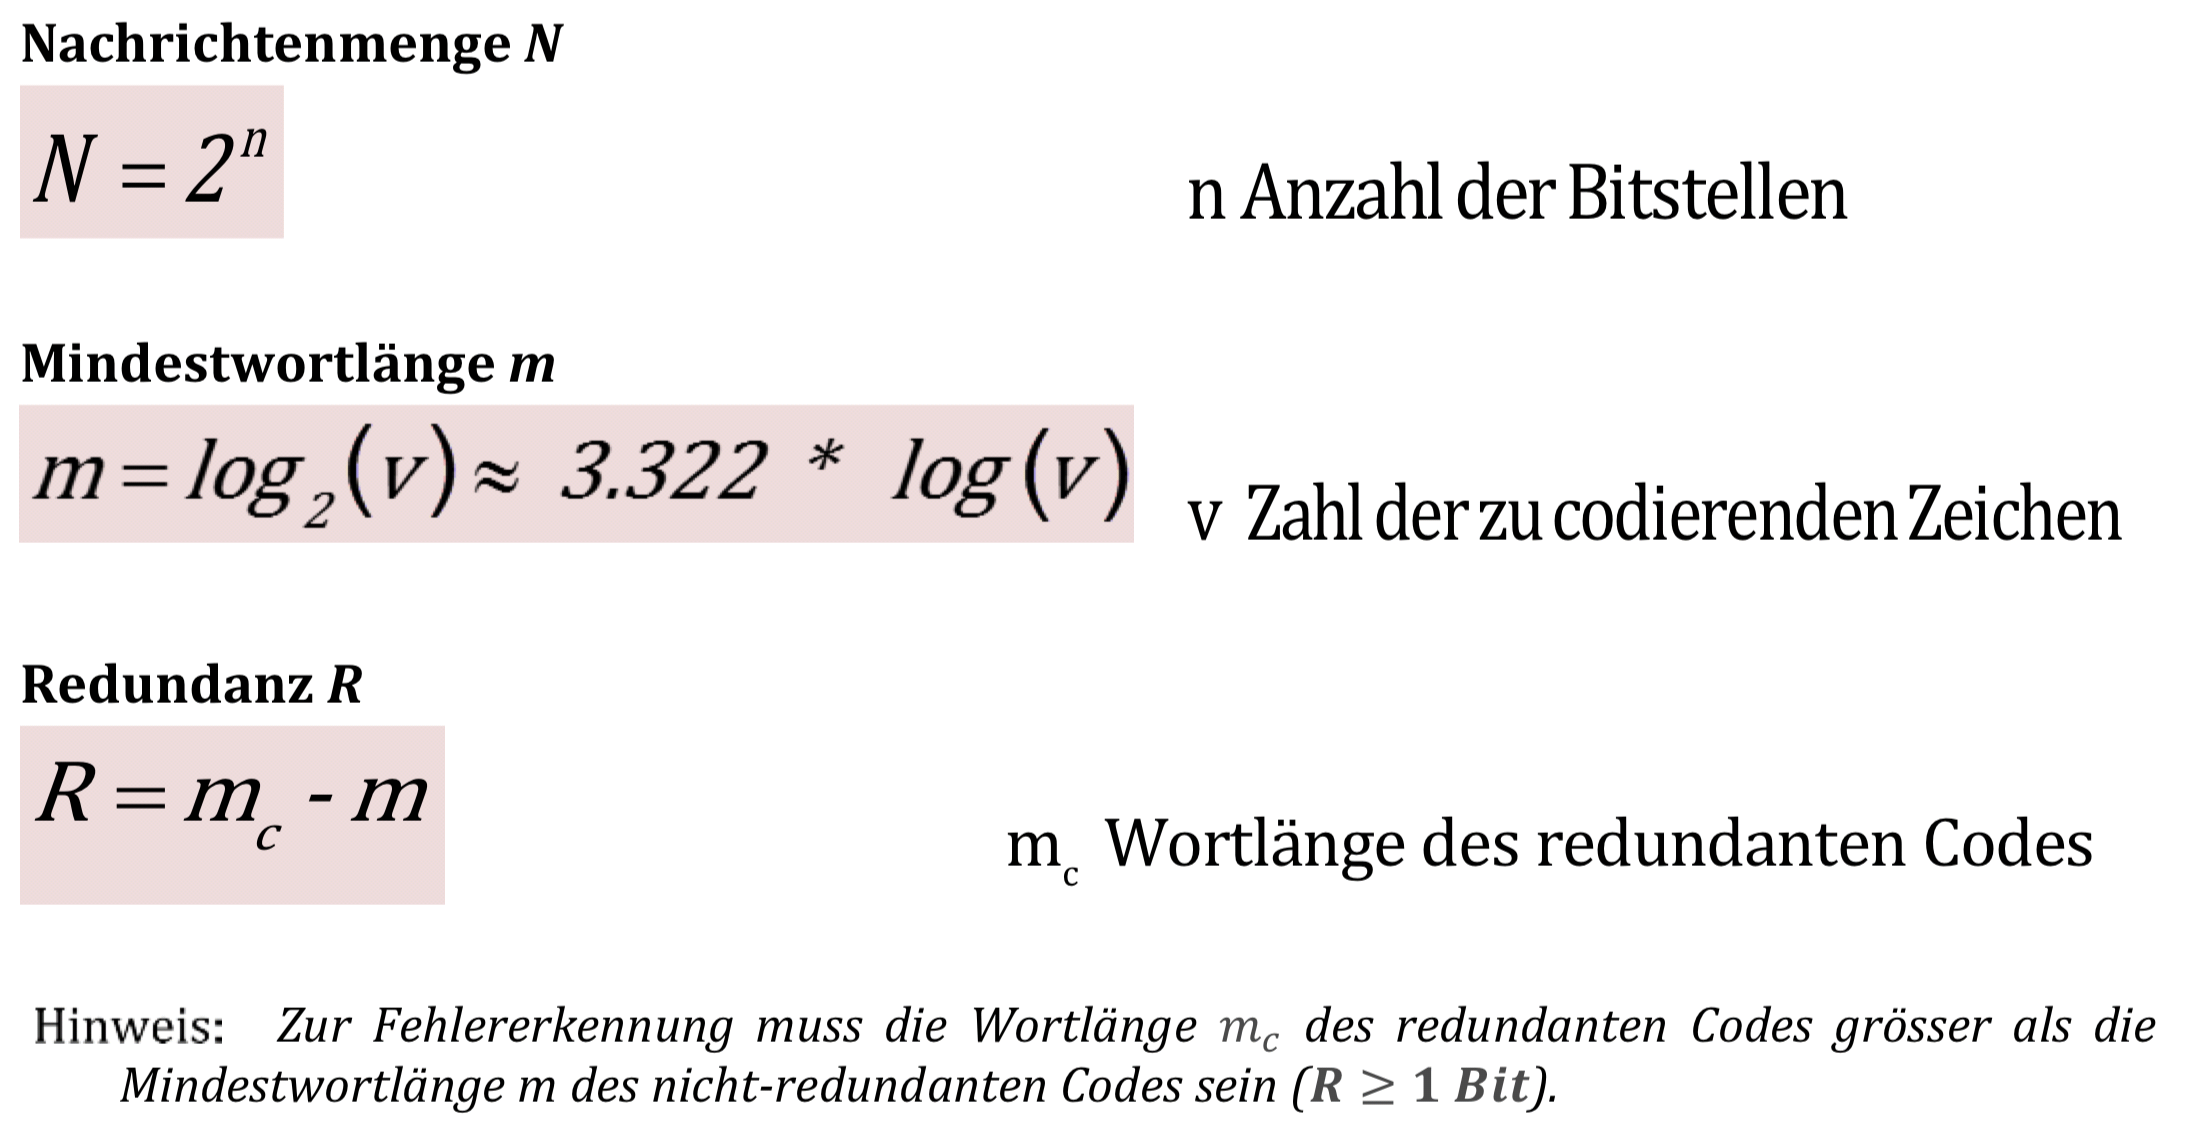
\includegraphics[width=9cm]{pics/2-Fehlererkennung1}\\
		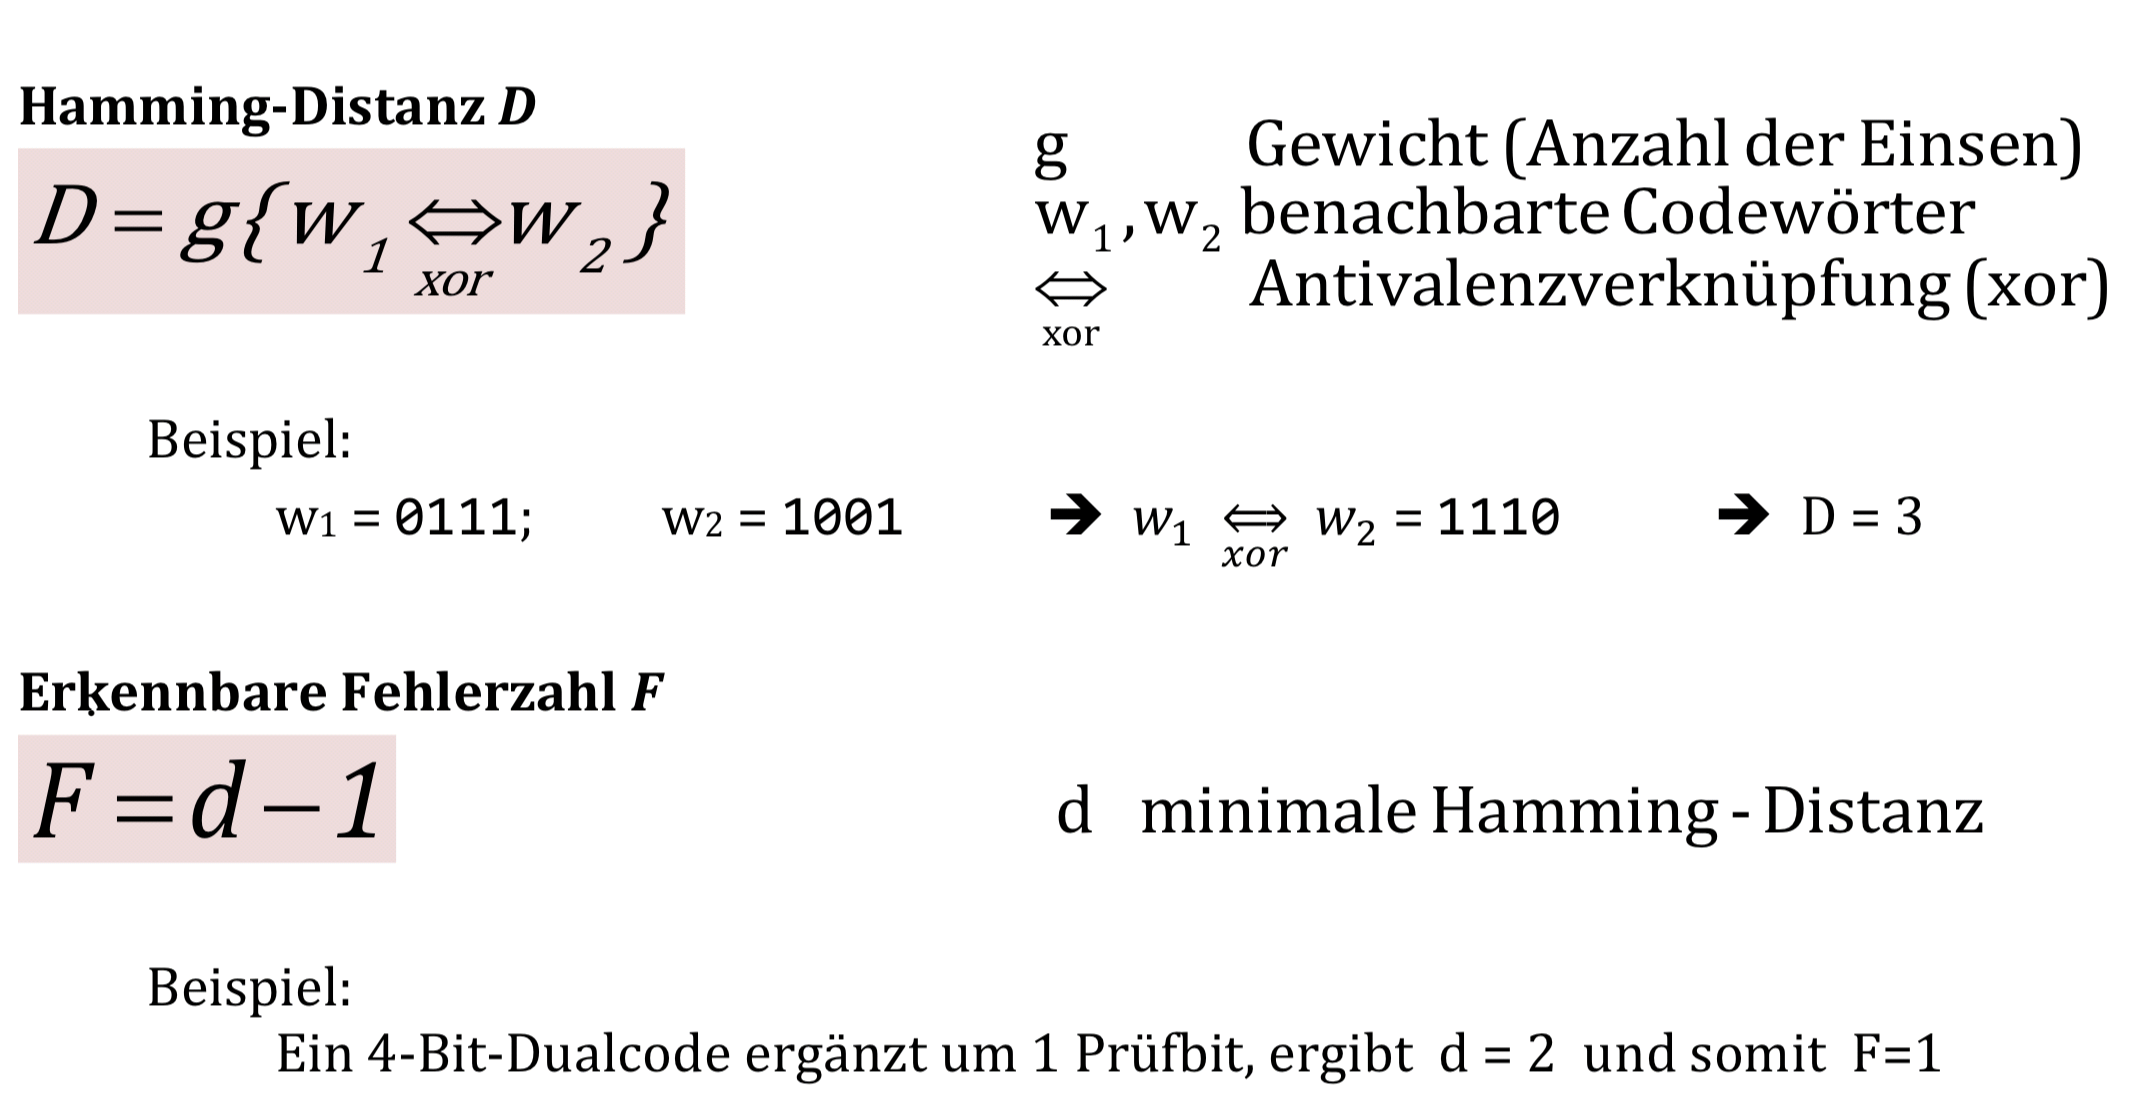
\includegraphics[width=9cm]{pics/2-Fehlererkennung2}
\end{minipage}
%
\begin{minipage}{0.5cm}
	\ \
\end{minipage}
%
\begin{minipage}{9cm}
	\subsubsection{Parity}
		Die in der Computer- und "Ubertragungstechnik weitverbreiteste und bekannteste Fehlererkennungsmethode ist das Parit"atsbit. Ein zus"atzliches Bit wird bei jedem g"ultigen Codewort z.B. auf eine gerade Parit"at erg"anzt. Damit wird jeder Einbit-Fehler an
			der ungeraden Summe von Einsen leicht erkennbar. Alle 
			g"ultigen Codeworte (inklusive Parit"atsbit) unterscheiden sich voneinander an mindestens zwei Stellen (Hamming-Distanz D=2).\\ 
			
	\begin{minipage}{6cm}
		\textbf{Definition Even und Odd Parity:}\\
		Das Parity-Bit wird in die $"$Z"ahlung der Einsen$"$ miteinbezogen, d.h. bei \textbf{Even Parity} wird das Parit"atsbit so gesetzt, dass die Anzahl Einsen inklusive Parity-Bit gerade ist: Eine ungerade Anzahl Einsen in einem Datenwort f"uhrt also zu einem Parity-Bit =1; damit
			wird die gesamte Anzahl Einsen gerade.\\
			 \textbf{Odd Parity} bedeutet: 
			Das Datenwort inklusive Parity-Bit besitzt eine ungerade 
			Anzahl Einsen.
	\end{minipage}
	%
	\begin{minipage}{0.2cm}
		\ \
	\end{minipage}
	%
	\begin{minipage}{2.6cm}
		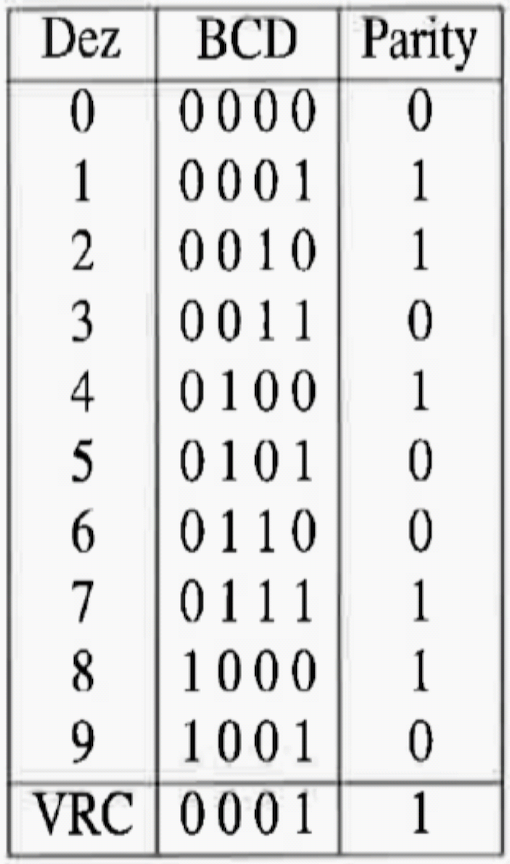
\includegraphics[width=2.6cm]{pics/2-Parity}\\
		\begin{small}
			\textit{Bsp. Even-Parity}
		\end{small}
	\end{minipage}
\end{minipage}

\subsubsection{CRC}
	\begin{minipage}{9cm}
		Das Problem der einfachen Parit"atspr"ufung besteht in ihrer Anf"alligkeit auf Mehrbitfehler: Sobald in einem mit Parity gesicherten Wort nicht nur ein, sondern zwei Bits gest"ort sind, kann dieser Fehler nicht erkannt werden. Die Fehlererkennungsrate bei einfacher Parity betr"agt nur 50\%, da alle geradzahligen Fehler nicht erkannt werden k"onnen.\\

		Mit der CRC-Technik (\textbf{Cyclic Redundancy Check}) k"onnen mit relativ wenig Aufwand Mehrfach- und Burst-Fehler (mehrere Fehler kurz hintereinander) in Datenbl"ocken entdeckt werden. Die CRC-Technik wird heute sehr verbreitet in der Datenspeicherung
			und der Daten"ubertragung (Computernetzwerke) angewendet.\\
	\end{minipage}
	%
	\begin{minipage}{0.5cm}
		\ \
	\end{minipage}
	%
	\begin{minipage}{9cm}
		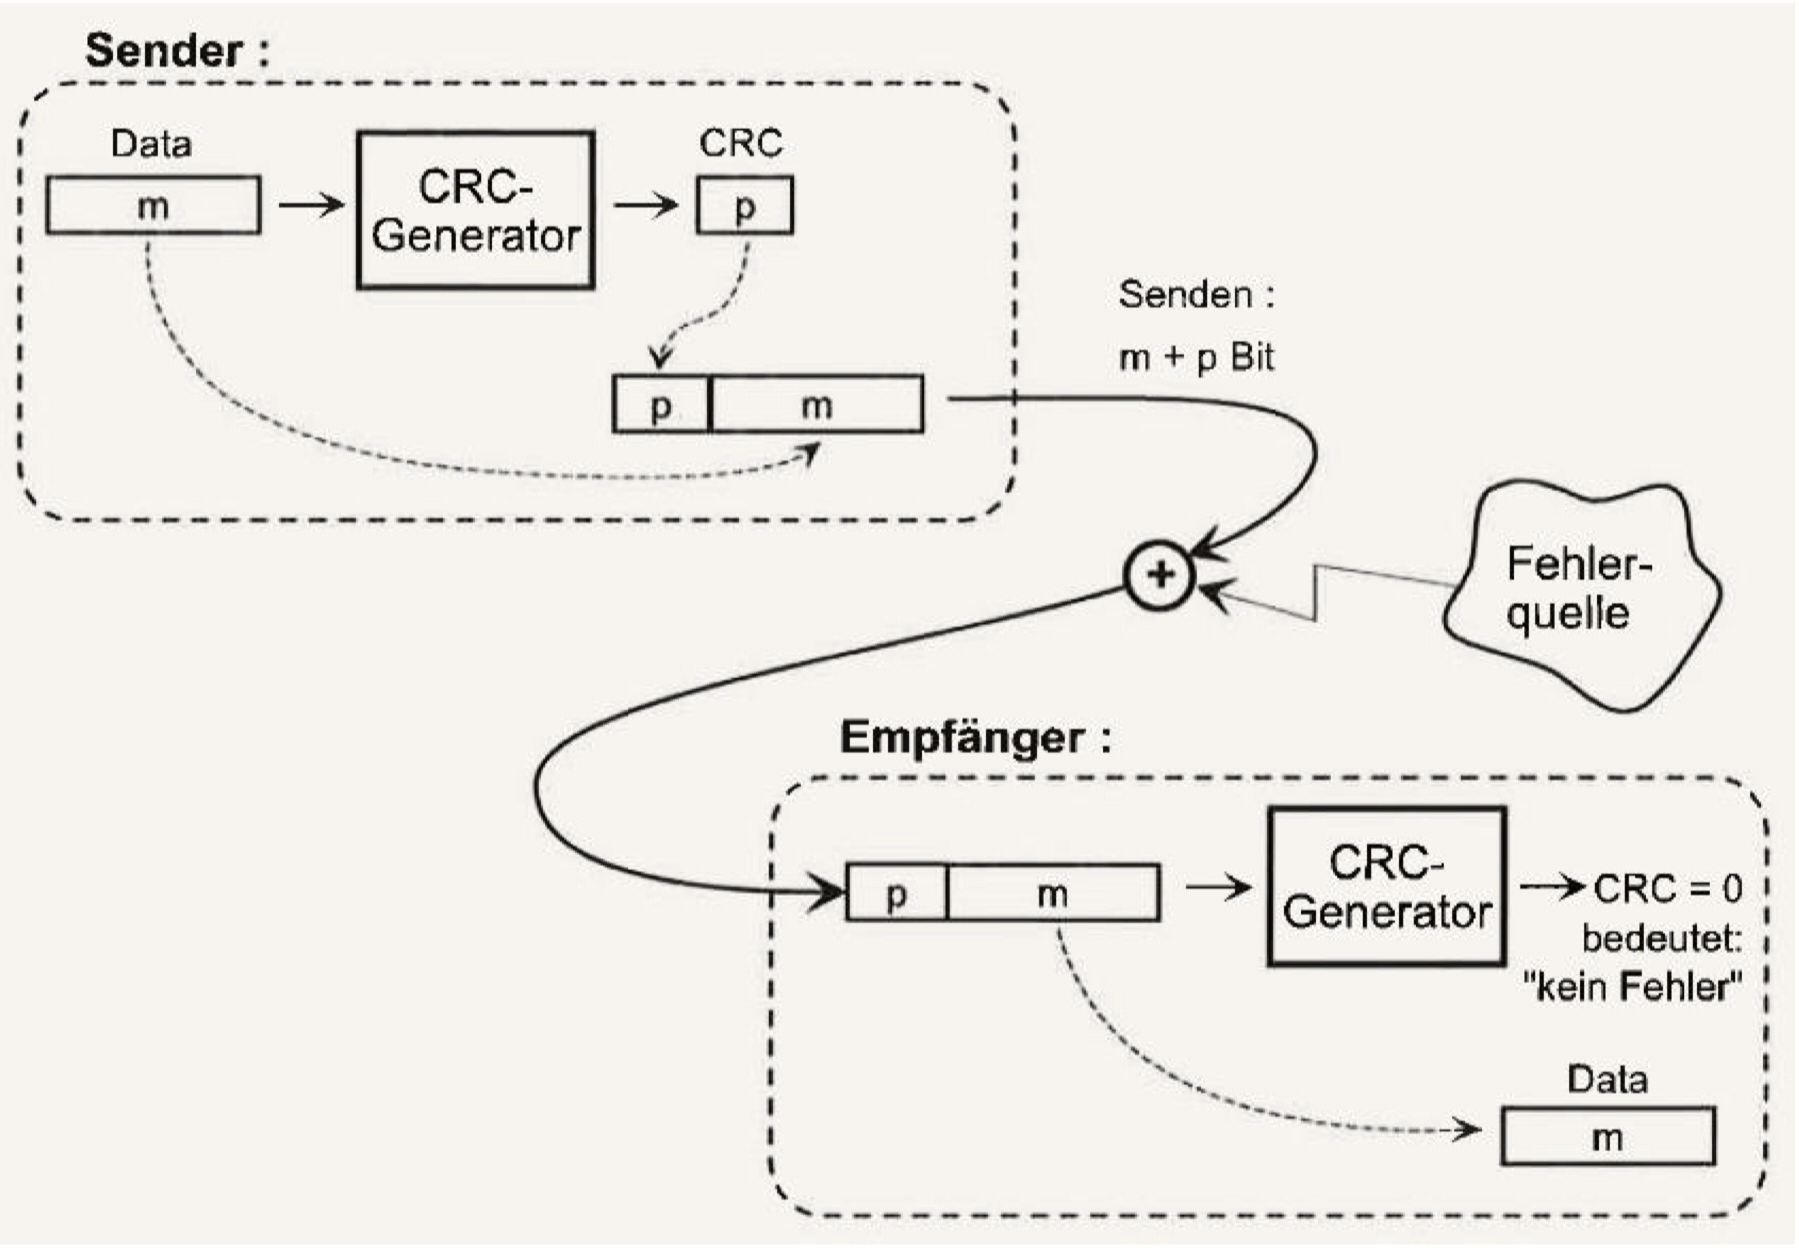
\includegraphics[width=8cm]{pics/2-CRC-Generator}
	\end{minipage}
	
	
\newpage

		
	\section{Aufbau und Funktionen}
\subsection{Komponenten eines Mikroprozessors}
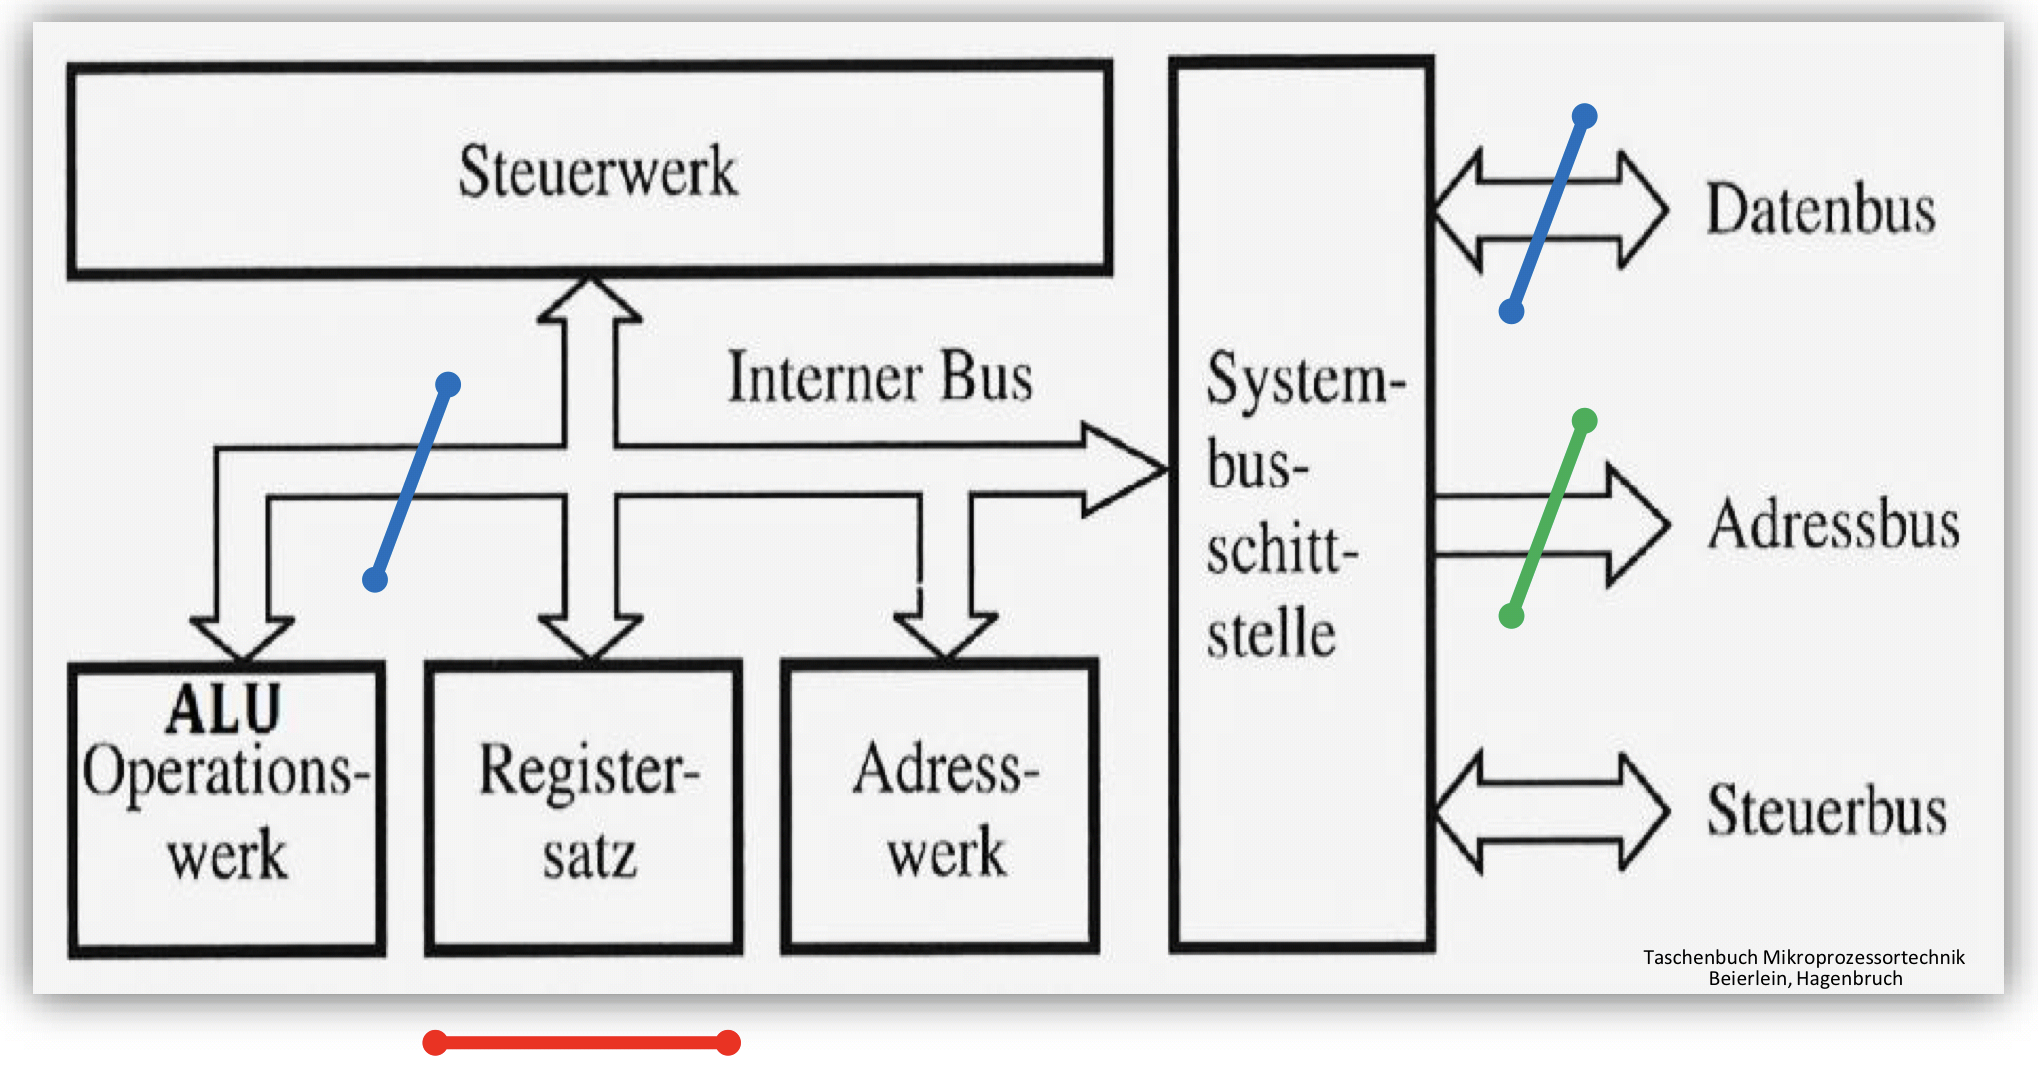
\includegraphics[width = 8cm]{pics/Komponenten-Mikroprozessor}

\begin{minipage}[t]{9cm}
	\subsubsection{Register}
	In enger Beziehung zur CPU befinden sich mehrere sehr schnell ansprechbare Register, die in ihrer Gesamtheit als Registersatz bezeichnet werden.\\
	Es wird mindestens ein \textbf{Akkumulator} ben"otigt (Universal-Register), der PicoBlaze hat sechzehn 8-Bit Universal-Register. Zudem hat der PicoBlaze sechzehn Adress-Register und auch noch Register wie Befehlsz"ahler(Program Counter, PC), Status-Register, Flags, Stackpointer usw.
\end{minipage}
%
\begin{minipage}{0.5cm}
	\ \
\end{minipage}
%
\begin{minipage}[t]{9cm}
	\subsubsection{Flags}
	Flags sind Attribute, welche das Ergebnis einer ALU-Operation zus"atzlich kennzeichnen. Die Flags befinden sich in einem Flag-Register und werden gesetzt wenn die Flag-Bedingung infolge einer ALU-Operation erf"ullt ist.
	
	Es gibt das \textbf{Zero-Flag}(Z), das \textbf{Carry-Flag}(C), das \textbf{Overflow-Flag}(V) und das \textbf{Negative-Flag}(N), eventuell gibt es noch weitere.
\end{minipage}

\begin{minipage}[t]{9cm}
	\subsubsection{ALU, Arithmetik-Logic Unit}
	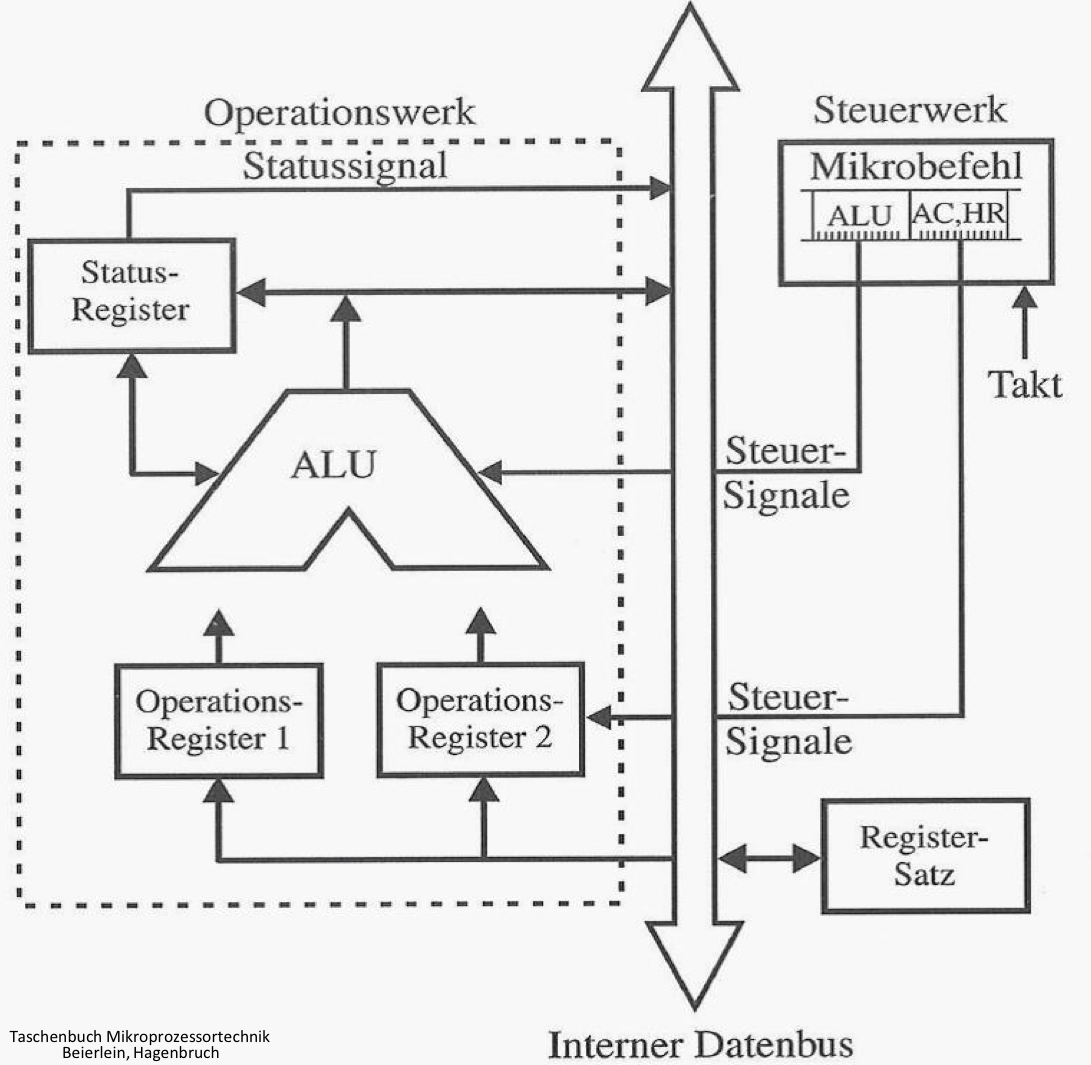
\includegraphics[width=6cm]{pics/ALU}\\
	Die \textbf{Arithmetic Logic Unit} "ubernimmt im Mikroprozessor die Datenverarbeitungsfunktion. Sie kann arithmetische Operationen wie \textbf{Addition, Subtraktion, Vergleiche}, logische Verkn"upfungen wie \textbf{AND, OR, XOR} und Verschiebungen von Bitstellen also \textbf{SHIFT} und \textbf{ROTATE}. Die Gr"osse der ALU-Operanden definiert die Einstufung des $\mu P$ als 8-, 16-, 32- oder 64-Mikroprozessor.
	
	\subsubsection{Systembus}
	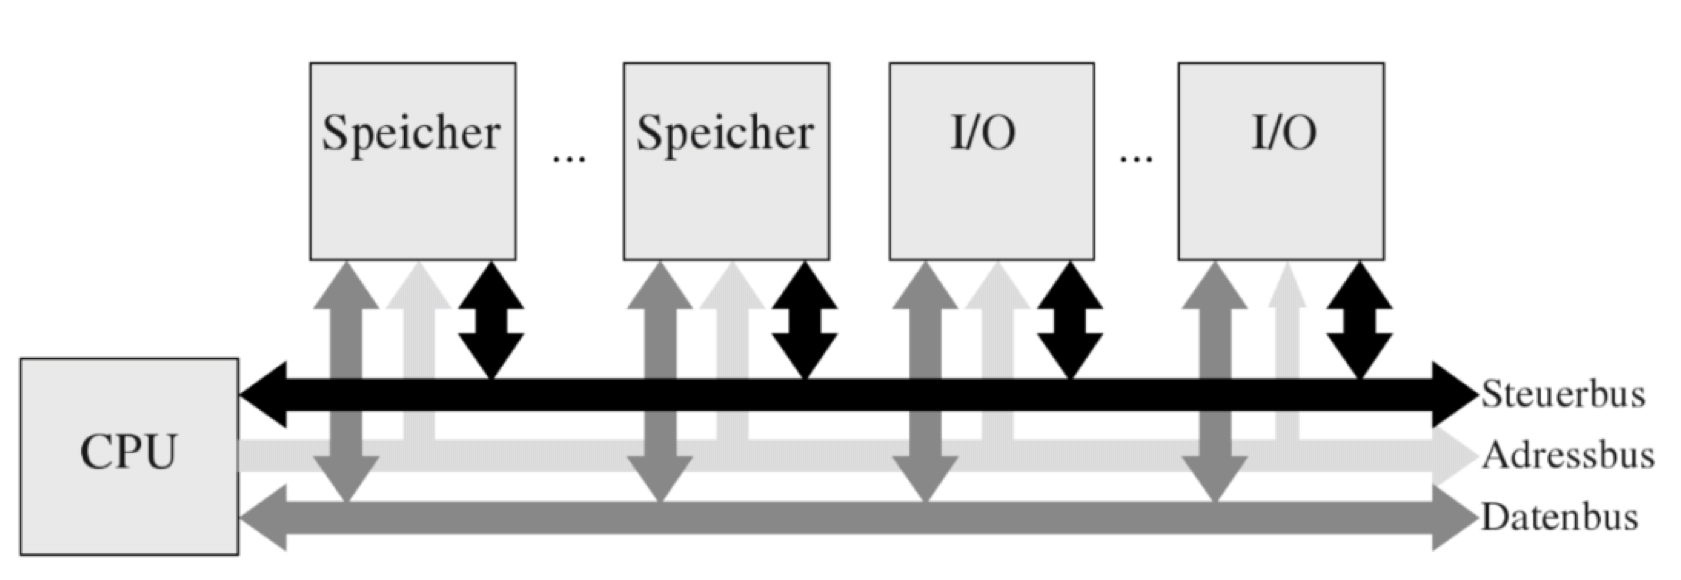
\includegraphics[width=7cm]{pics/Systembus}\\
	Die Teilbusse Datenbus, Adressbus und Steuerbus bilden gemeinsam den Systembus des Mikrocontrollers. Die Bus-Spezifikation besteht aus Funktionsbeschreibung und Operationen, elektrische Eigenschaften, zeitliche Eigenschaften usw..

\end{minipage}
%
\begin{minipage}{0.5cm}
	\ \
\end{minipage}
%
\begin{minipage}[t]{9cm}
	\subsubsection{Steuerwerk, Control Unit}
	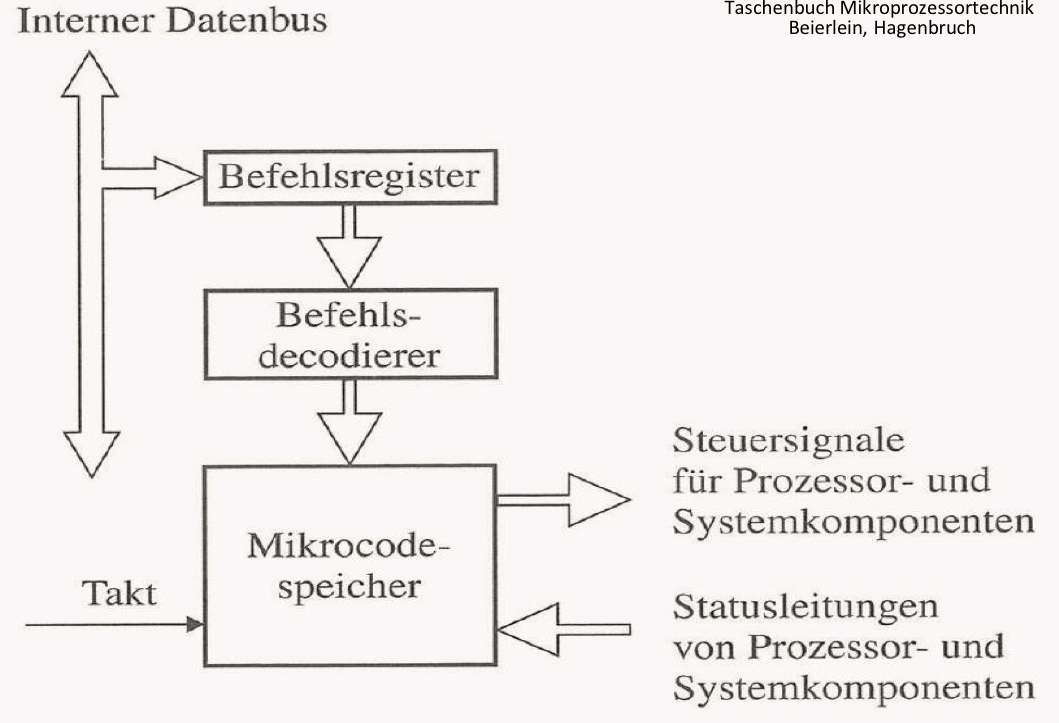
\includegraphics[width=7cm]{pics/Befehlsregister}
	
	Das \textbf{Steuerwerk} steuert im Zeitraster des Taktsignals alle Abl"aufe innerhalb der CPU und den gesamten Informationsaustausch auf dem internen Bus, sowie auf dem Datenbus zwischen CPU und Speicher- bzw. Eingabe-/Ausgabe-Einheiten.
	
	Aufgaben des Steuerwerkes:
	\begin{itemize}
		\item Steuerung aller prozessinternen Abl"aufe
		\item Bereitstellung von Adress-Informationen
		\item Steuerung der Abl"aufe auf dem Systembus
	\end{itemize}

	Der \textbf{Befehlsz"ahler (Program Counter, PC)} enth"alt stets die aktuelle Befehlsadresse. Bei jedem Befehlswortzugriff wird der PC um die entsprechende Befehlsgr"osse inkrementiert.
	
	\subsubsection{Adresswerk, Address Unit}
	Das Adresswerk berechnet nach den Vorschriften des Steuerwerks die Adresse der geforderten Operanden oder auszuf"uhrenden Befehle im Speicher.
\end{minipage}

\subsection{Ausgew"ahlte Funktionsprinzipien}
F"ur die Beschreibung der Funktionsprinzipen wird ein \textbf{Von-Neumann-Rechner} verwendet.

\begin{minipage}[t]{8cm}
	\subsubsection{Befehlsabarbeitung}
	Der \textbf{Instruction Code} wird in einer Endlos-Schleife ausgef"uhrt.\\
	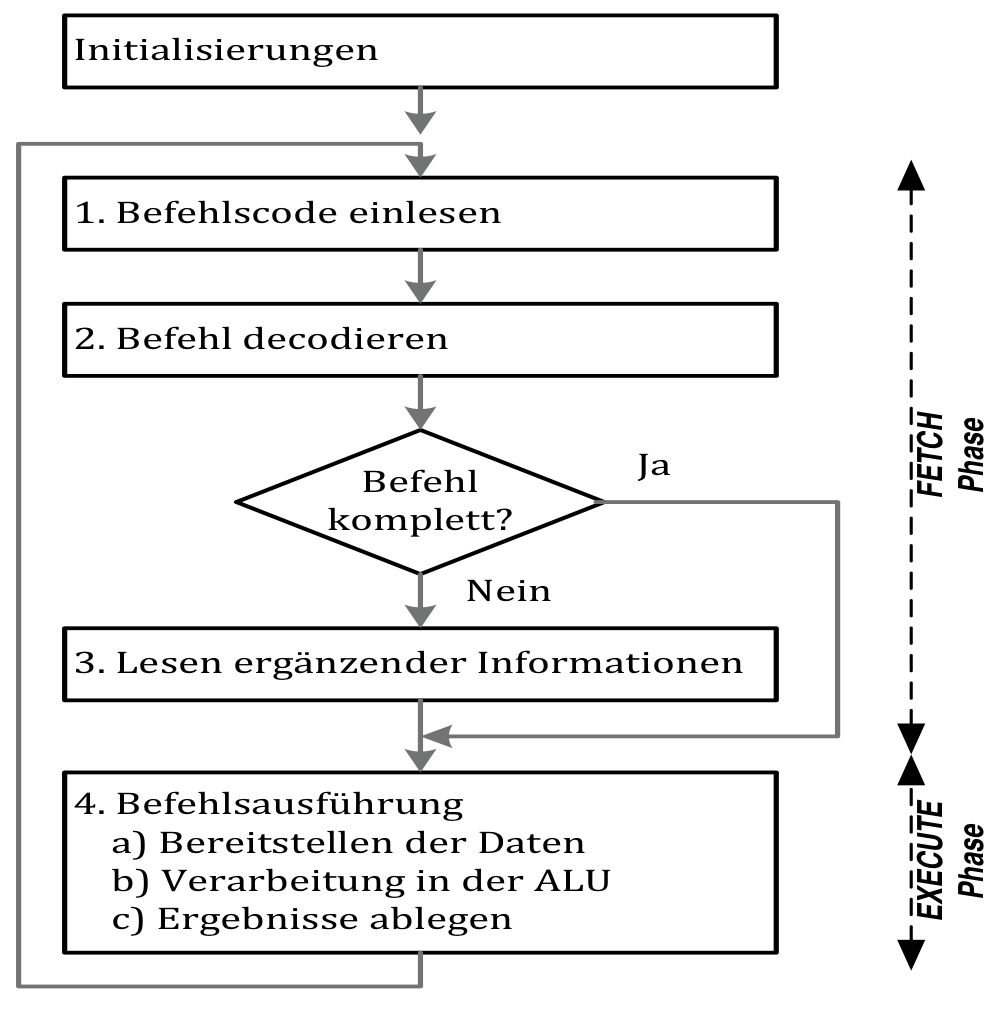
\includegraphics[width=5cm]{pics/Befehlablauf}
\end{minipage}
%
\begin{minipage}{0.5cm}
	\ \
\end{minipage}
%
\begin{minipage}[t]{10cm}
	\subsubsection{Bussteuerung}
	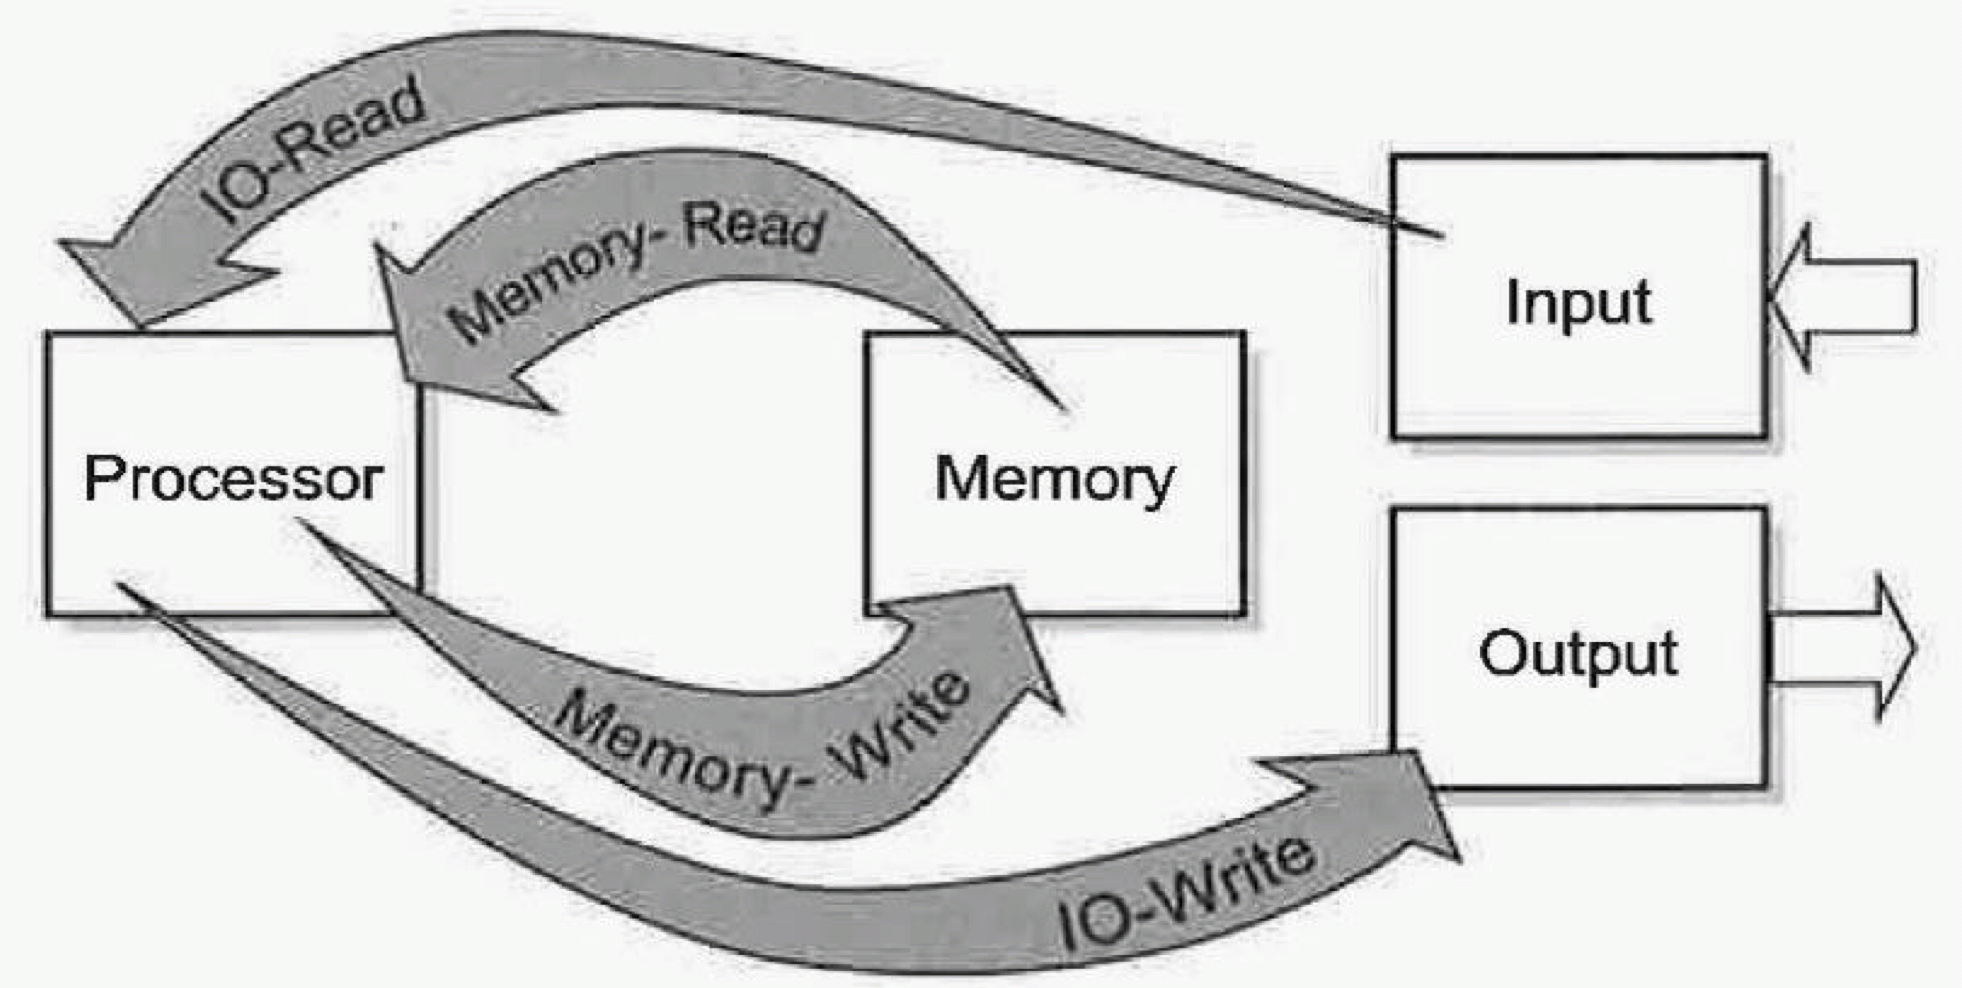
\includegraphics[width=6cm]{pics/Bus-Operationen}\\
	Man sieht, dass alle Transfers "uber den Prozessor gehen, eine Ausnahme bilden Peripherien mit DMA-Funktionalit"at, welche die Master-Funktion vor"ubergehend "ubernehmen k"onnen.
	Zudem gibt es den \textbf{asynchronen Systembus}, bei welchem mit speziellen Steuersignalen die Synchronasitation hergestellt wird und den \textbf{Synchronen Systembus}, bei welchem mit einem gemeinsamen Bustakt synchronisiert wird.
\end{minipage}
	
\begin{minipage}[t]{8cm}
	\subsubsection{Ankopplung von Eingabe und Ausgabe-Einheiten}
	Damit Peripherien an einen Mikroprozessor angeschlossen werden k"onnen ben"otigt es Interface-Bausteine, welche wesentlich aus zwei Komponenten bestehen, aus der Elektronik zur Ankopplung an den Bus des Mikroprozessors und aus einer konfigurierbaren Elektronik zur Ankopplung der externen Komponenten.\\
	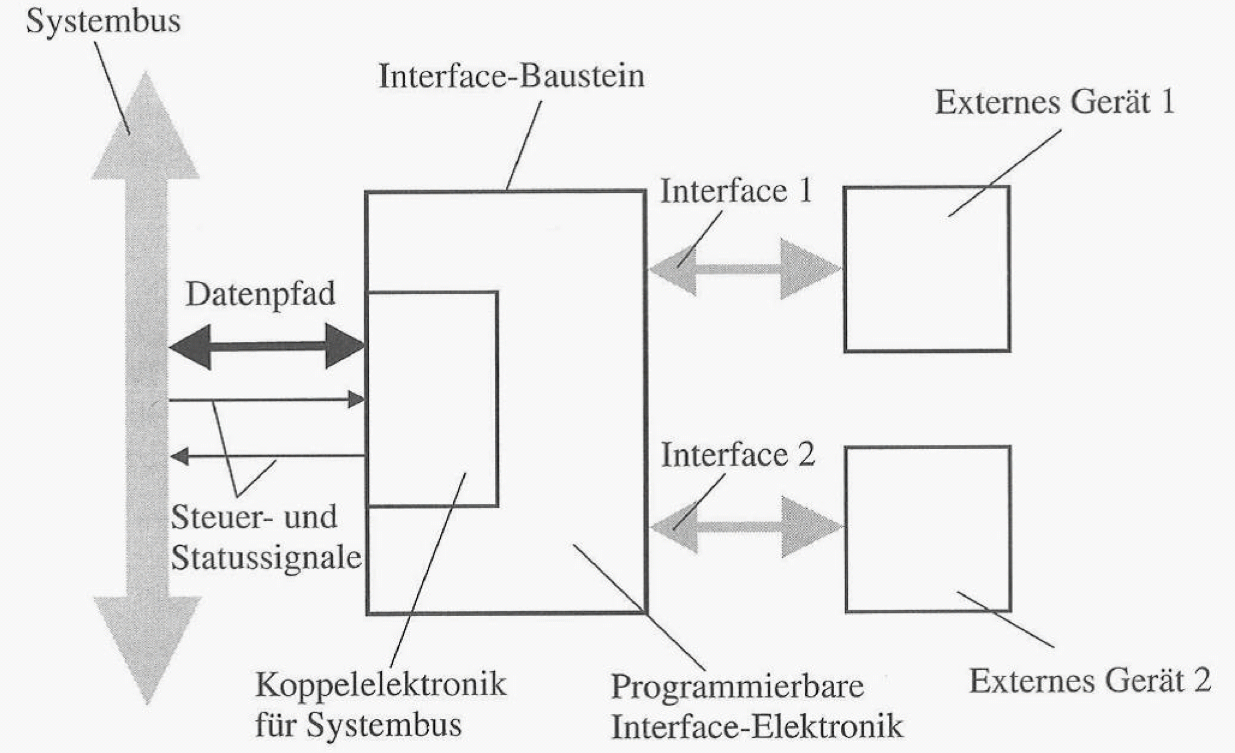
\includegraphics[width=5.5cm]{pics/Interface-Komponenten}
\end{minipage}
% 
\begin{minipage}{0.5cm}
	\ \
\end{minipage}
%
\begin{minipage}[t]{10cm}
	\subsubsection{Memory-Mapped I/O}
	Bei der Ansteuerung der Interface-Bausteine als I/O-Komponenten bieten sich zwei grunds"atzliche Konzepte an:\\
	\textbf{Isolierte Adressierung:} Separater Adressraum f"ur I/O und Speicher. Verschiedene Prozessor-Instruktionen (z.B. /MEMR, /MEMW oder /IOR, /IOW).\\
	\textbf{Memory-Mapped I/O:} Der Adressraum von I/O und Speicher ist nicht getrennt. Ansprechung durch dieselben Prozessor-Instruktionen.\\
	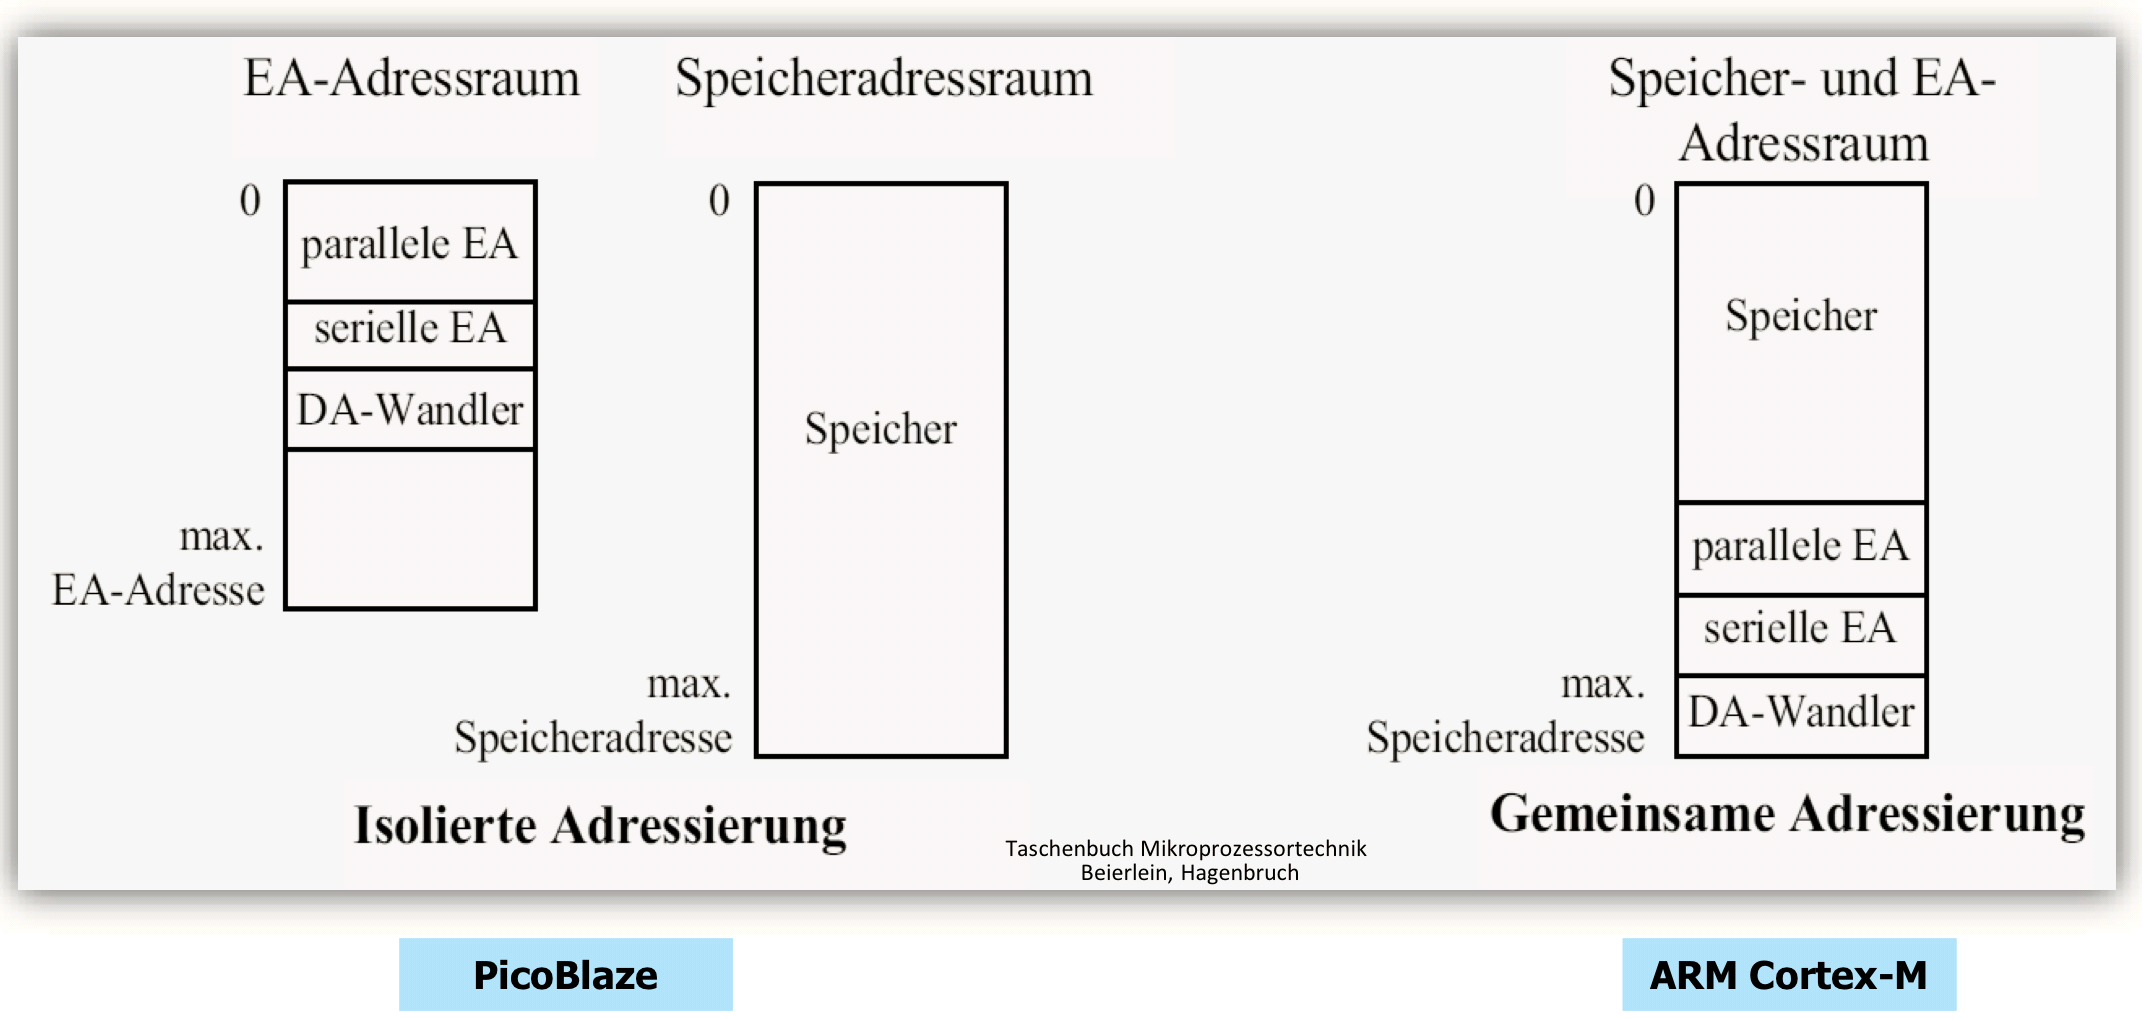
\includegraphics[width=7.5cm]{pics/Adressbereich}
\end{minipage}

\begin{minipage}[t]{8cm}
	\subsubsection{Stack-Funktion}
	Der \textbf{Stapelspeicher (Stack)}, ist ein reservierter Speicherbereich, der mittels Stack Pointer, SP, nach dem Last-In-First-Out-Prinzip (LIFO) verwaltet wird. Mit dem \textbf{PUSH} Befehl k"onnen Daten-Elemente dem Stack hinzugef"ugt werden und mit dem \textbf{POP} Befehl k"onnen sie wieder entnommen werden.\\
	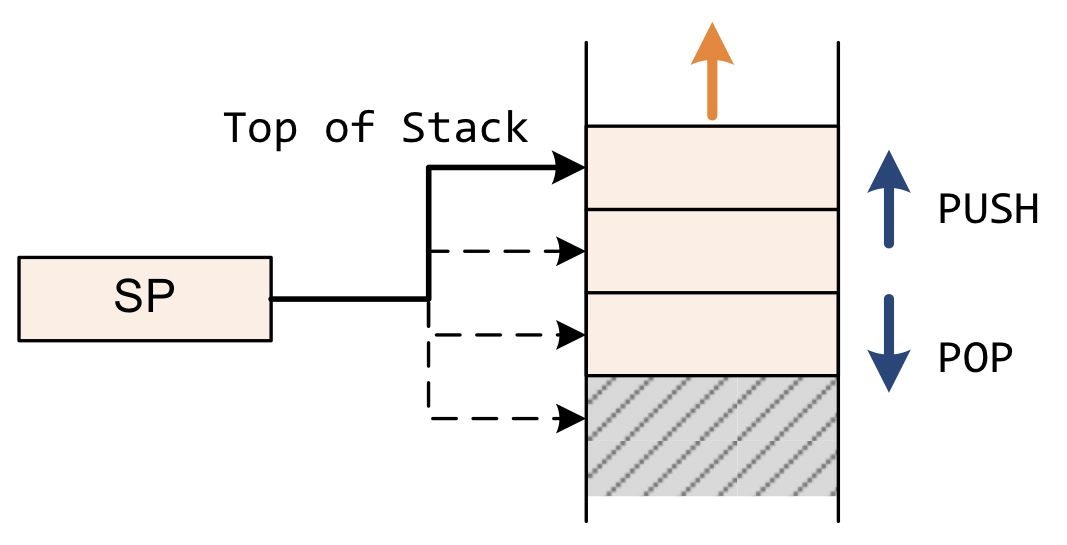
\includegraphics[width=5cm]{pics/Stack-Operationen}
\end{minipage}
%
\begin{minipage}{0.5cm}
	\ \
\end{minipage}
%
\begin{minipage}[t]{10cm}
	\subsubsection{Polling vs. Interrupt-Steuerung}
	Beim \textbf{Polling}-Verfahren wird per Programm immer kontrolliert wie die Status-Informationen aussehen und so festgestellt ob Daten von Eingabe-Einheiten eingelesen oder an Ausgabe-Einheiten ausgegeben werden k"onnen.\\
	Beim \textbf{Interrupt}-Verfahren k"onnen Ein-/Ausgabe-Einheiten eine Bedienungsanforderung per Interrupt-Request anmelden. Diese trifft asynchron ein und der Mikroprozessor entscheidet "uber den Ausf"uhrungszeitpunkt der Interrupt-Service-Routine (ISR).
		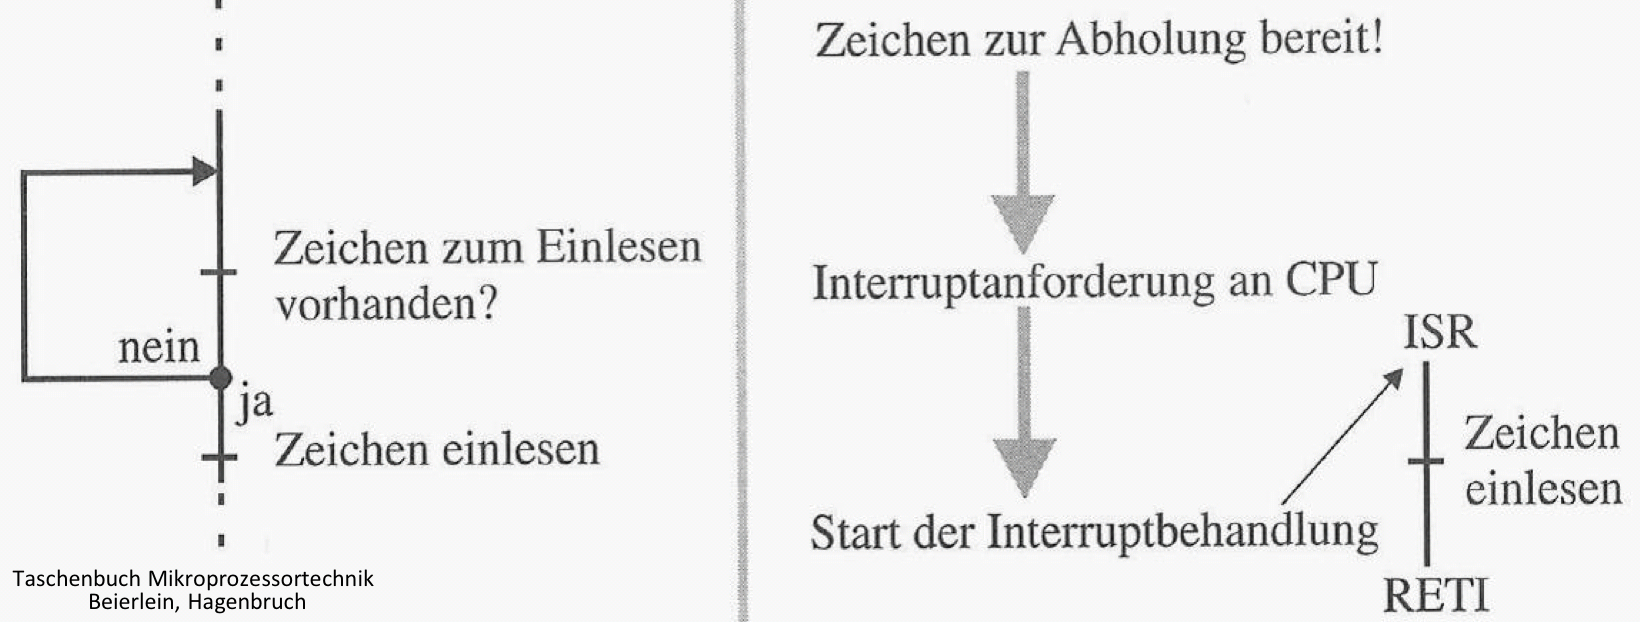
\includegraphics[width=7cm]{pics/Interrupt-operationen}
\end{minipage}

\subsection{Basis-Architekturen}
\begin{minipage}{9cm}
	\textbf{CISC-Prozessoren}(Complex Instruction Set Computer):\\
	Traditionelle Prozessoren sind nach dem CISC-Modell realisiert. CISC-Prozessoren besitzen in der Regel eine Befehlssatz mit vielen spezialisierten und leistungsf"ahigen Instruktionen.
\end{minipage}
%
\begin{minipage}{0.5cm}
	\ \
\end{minipage}
%
\begin{minipage}{9cm}
	\textbf{RISC-Prozessoren}(Reduced Instruction Set Computer):
	Sie besitzen einen kleinen (reduzierten) Befehlssatz (< 100 Befehle). Die Maschinenbefehle sind sehr einfach und kurz gehalten. Kompliziertere Befehle m"ussen aus mehreren einfachen Einzelbefehlen zusammengesetz werden.
\end{minipage}

	
	
	\section{Allgemeines Programmiermodell}
Dieser Abschnitt soll dazu dienen einen allgemeinen "Uberlick "uber die Assemblerprogrammierung zu erhalten, da sich die Programmiermodelle unter den Mikroprozessoren variieren.
\subsection{Begriffserkl"arung}
\begin{minipage}{10cm}
	Der Mikroprozessor stellt den Anwender zur Programmierung den \textbf{Maschincode} zur Verf"ugung. Der Maschinencode besteht aus \textbf{Bitfolgen}, welche das Steuerwerk des Prozessors als Befehle interpretiert, auswertet und danach Aktionen ausf"uhrt. Die einzelnen Befehle sind bin"ar codiert und werden aus dem \textbf{Programmspeicher} heraus der CPU zur Ausf"uhrung bereitgestellt.\\
	
	Die \textbf{Assemblersprache} ist eine maschinenorientierte Sprache. Durch Abk"urzungen (\textbf{Mnemonics}) wird das Programmieren vom bin"are Maschinencode erleichtert.\\
	
	Das \textbf{Assemblier-Program} "ubersetzt Assembler Sprache in bin"aren Maschinencode.\\
	
	Bei der hardwarenahen Programmierung verwendet der Programmierer das \textbf{Registermodell} und \textbf{Befehlssatz} des verwendeten Prozessors.
\end{minipage}
%
\begin{minipage}{0.5cm}
	\ \
\end{minipage}
%
\begin{minipage}{8cm}
	\includegraphics[width = 8cm]{pics/Programmiermodell}
\end{minipage}
	
\subsection{Registersatz}
Als \textbf{Registersatz} bezeichnet man die mittels Maschinenbefehle direkt ansprechbaren Register eines Mikroprozessors.

\subsection{Adressierungsarten}
Die Adressierungsart ist der Algorithmus, wie eine Adresse eines Operanden berechnet wird. Durch den geschickten Einsatz von Adressierungsarten k"onnen Programmieraufgaben effizient und elegant gel"ost werden.

\subsubsection{Unmittelbare Adressierung (Immediate Addressing)}
Bei dieser Adressierungsart ist der betroffene Operand eine Konstante, die im Anschluss am dem OpCode im Speicher steht.
\begin{minipage}{2cm}
	\includegraphics[width=2cm]{pics/Unmittelbare-Adressierung}
\end{minipage}
%
\begin{minipage}{0.5cm}
	\ \
\end{minipage}
%
\begin{minipage}{9cm}
	\textbf{Beispiel:}\\
	\includegraphics[width=9cm]{pics/UnmittelbareAdressierung-Bsp}
\end{minipage}

\subsubsection{Absolute Adressierung (Direct Addressing, Absolute Addressing)}
Ein absolut adressierter Operand ist ein Wert an einer bestimmten Speicheradresse, die im Befehl mit angegeben wird.
\begin{minipage}{4cm}
	\includegraphics[width=4cm]{pics/Absolute-Adressierung}
\end{minipage}
%
\begin{minipage}{0.5cm}
	\ \
\end{minipage}
%
\begin{minipage}{9cm}
	\textbf{Beispiel:}\\
	\includegraphics[width=9cm]{pics/Absolute-Adressierung-Bsp}
\end{minipage}

\subsubsection{Explizite Register Adressierung (Register Direct Addressing)}
Bei der expliziten Register Adressierung ist der Operand Inhalt eines Prozessorregisters. Es k"onnen universelle Register, Datenregister, Adressregister und auch spezielle Register wie Stackpointer und Statusregister angesprochen werden.
\begin{minipage}{5cm}
	\includegraphics[width=5cm]{pics/Explizite-Adressierung}
\end{minipage}
%
\begin{minipage}{0.5cm}
	\ \
\end{minipage}
%
\begin{minipage}{9cm}
	\textbf{Beispiel:}\\
	\includegraphics[width=9cm]{pics/Explizite-Adressierung-Bsp}
\end{minipage}

\subsubsection{Indizierte Adressierung (Indexed Addressing)}
Wird anstatt einer konstanten eine variable Adressdistanz ben"otigt, die erst zur Laufzeit eines Programmes feststeht, so wird die \textbf{indizierte Adressierung} verwendet.\\
Die effektive Adresse wird hier aus der Basisadresse (A1) in einem Adressregister und einem Adressversatz aus einem weiteren Register berechnet. Bei manchen Prozessoren ist daf"ur ein spezielle Indexregister vorhanden.

\begin{minipage}{7cm}
	\includegraphics[width=7cm]{pics/Indizierte-Adressierung}
\end{minipage}
%
\begin{minipage}{0.5cm}
	\ \
\end{minipage}
%
\begin{minipage}{9cm}
	\textbf{Beispiel:}\\
	\includegraphics[width=9cm]{pics/Indizierte-Adressierung-Bsp}
\end{minipage}

\subsubsection{Implizite Register Adressierung (Implied Register Addressing)}
\begin{minipage}{9cm}
	Einige Befehle benutzen \textbf{implizite Operanden}, d.h. eine ausdr"uckliche Angabe der Operanden ist gar nicht erforderlich. Der Kontext des Befehls definiert die erforderlichen Operanden vollst"andig.  So verwenden beispielsweise einige arithmetische Befehle implizit den Akkumulator oder ein anderes Register.
\end{minipage}
%
\begin{minipage}{0.5cm}
	\ \
\end{minipage}
%
\begin{minipage}{9cm}
	\textbf{Beispiel:}\\
	\includegraphics[width=9cm]{pics/Implizite-Register-Adressierung-Bsp}
\end{minipage}

\subsection{Befehlssatz/Befehlsgruppen}
Der \textbf{Befehlssatz (Instruction Set)} umfasst alle Maschinenbefehle, welche der Mikroprozessor ausf"uhren kann. Der Befehlssatz ist dem Aufbau und der Prozessorarchitektur angepasst.\\
Der Befehlssatz ist in einer \textbf{Befehlsliste} spezifiziert.

\subsection{Debug-Unterst"utzung}
Die meisten Prozessoren bieten als Debug-Unterst"utzung den \textbf{Trap-Mechanismus} an. Dabei wird bei der Ausf"uhrun eines Befehls eine Unterbrechungsroutine aufgerufen, die dann die Auswirkungen des Befehls interpretieren und anzeigen kann.\\
Verschiedene Prozessoren bieten dar"uber hinaus weitergehende Features an.

\subsection{Einf"uhrung in die Programmierung}
Der \textbf{Befehlssatz} eines Prozessors ist die Menge der Befehlscodes, die der jeweilige Prozessor direkt, d.h. ohne weitere Konvertierung oder Interpretierung ausf"uhren kann.

\textbf{Mnemonics:} Aus einpr"agsamen Abk"urzungen zusammengesetzte Befehlscodes

\textbf{Assemblierung:} "Ubersetzung von Assemblersprache in Maschinensprache 

\textbf{Disassemblierung:} "Ubersetzung von Maschinensprache in Assemblersprache 

\subsubsection{Code-Beispiel}
\begin{minipage}[t]{6cm}
	\textbf{Grundlegender Programmablauf:}\\
	\includegraphics[width=6cm]{pics/Bsp-Programmablauf}
\end{minipage}
%
\begin{minipage}{0.25cm}
	\ \
\end{minipage}
%
\begin{minipage}[t]{6cm}
	\textbf{Assemblerprogramm 68000:}\\
	\includegraphics[width=6cm]{pics/Bsp-Assembler}
	
\end{minipage}
%
\begin{minipage}{0.25cm}
	\ \
\end{minipage}
%
\begin{minipage}[t]{6cm}
	\textbf{Maschinencode im Speicher:}\\
	\includegraphics[width=6cm]{pics/Bsp-Maschinencode}
\end{minipage}	

	\section{PicoBlaze}
\begin{minipage}{9cm}
	\vspace{-4ex}
	Der PicoBlaze ist ein 8-Bit-RISC-Mikrocontroller-Kern. Er ist limitiert auf \textbf{1K Instruktionen}, besitzt von Grund auf nur das Carry- und Zero-Flag und verzichtet auf den Software-Stack.

Beim PicoBlaze kann mit der Clock-Frequenz bis hinunter zu 0Hz gefahren werden und alle Instruktionen werden immer in zwei Taktzyklen ausgef"uhrt.

Der PicoBlaze ist in einem FPGA eingebettet und bietet somit die optimale Balance zwischen den beiden.
\end{minipage}
%
\begin{minipage}{0.5cm}
	\ \
\end{minipage}
%
\begin{minipage}{8cm}
	\includegraphics[width=8cm]{pics/PicoBlaze-Pro-Cons}
\end{minipage}

\subsection{Aufbau} 
\begin{minipage}{9cm}
	\vspace{-12ex}
	Der PicoBlaze verf"ugt "uber 16 \textbf{General-Purpose Register}, welche alle 8-Bit breit sind.
 	Die Verarbeitungsgr"osse der ALU betr"agt 8Bit, dabei werden alle operationen mit einem General-Purpose Regsiter (sX) als ersten Operanden durchgef"uhrt, das Resultat der Operation wird im selben Register (sX) abgelegt.
\end{minipage}
%
\begin{minipage}{0.5cm}
	\ \
\end{minipage}
%
\begin{minipage}{9cm}
	\includegraphics[width=9cm]{pics/PicoBlaze-Aufbau}
\end{minipage}
  
\subsection{Instruktionssatz}
\begin{minipage}{9cm}
	Alle Instruktionen des PicoBlaze Mikrocontrollers sind in einem einheitlich breiten Bitmuster, n"amlich 18 Bit breit. Dabei sind die Instruktionen als 0-, 1- oder 2-Adress-Befehle implementiert, wobei f"ur den Operand 1 bzw. Operand 2 je nach Instruktion unterschiedliche Angaben ben"otigen. Die Spezifikation eines Operanden kann ein direkter Zahlenwert sein oder sich auf die Bezeichnung ind den verschiedenen Adressbereichen beziehen.\\

	Der PicoBlaze hat nur wenige Adressbereiche, wie "ublich f"ur RISC-Prozessorkerne. Auf diese Adressbereiche kann nur mit klar festgelegten Instruktionsklassen und zugeh"origen Adressierungsarten zugegriffen werden.
\end{minipage}
%
\begin{minipage}{0.5cm}
	\ \
\end{minipage}
%
\begin{minipage}{9cm}
	\includegraphics[width=5cm]{pics/PicoBlaze-OpGroesse}\\
	
	\includegraphics[width=8cm]{pics/PicoBlaze-Adressierung}
\end{minipage}

\subsection{Instruktionscodierung}
\begin{minipage}{9cm}
	Die Informationen zu den Operanden ist immer in den gleichen Bit-Bereichen lokalisiert. Bei der Disassemblierung von Instruction Codes gehen Kommentare und Labels verloren. Die Instruction Codes werden immer als Hexadezimale dargestellt. Mit den obersten 6-Bit (17-12) des Instruction Codes kann mit dem PicoBlaze Instruction Set (Quick-Reference) der Befehl lokalisiert werden.
\end{minipage}
%
\begin{minipage}{0.5cm}
	\ \
\end{minipage}
%
\begin{minipage}{9cm}
		\begin{tabular}{|l|l|l}
			\cline{1-2}
			\rowcolor[HTML]{C0C0C0} 
			\textbf{Operanden-Information} & \textbf{Bit}        & \cellcolor[HTML]{FFFFFF}{\color[HTML]{FFFFFF} \textbf{}} \\ \cline{1-2}
			Register sX                    & 11-8                        & \cellcolor[HTML]{F8FF00}x                                \\ \cline{1-2}
			Register sY                    & 7-4                         & \cellcolor[HTML]{34FF34}y                                \\ \cline{1-2}
			Absolute instruction address   & 9-0                         & \cellcolor[HTML]{34CDF9}a                                \\ \cline{1-2}
			Immediate Constant             & 7-0 						& \cellcolor[HTML]{F8A102}k                                \\ \cline{1-2}
			Port address                   & 7-0                         & \cellcolor[HTML]{FF00A9}p                                \\ \cline{1-2}
			Scratchpad RAM address         & 5-0                         & \cellcolor[HTML]{9B9B9B}s                                \\ \cline{1-2}
		\end{tabular}
\end{minipage}

\textbf{Beispiele:}
\begin{table}[h!]
\begin{tabular}{|lll|lll|llllll|}
\hline
\multicolumn{3}{|l|}{\cellcolor[HTML]{C0C0C0}\textbf{Assembler-Befehl}}                  & \multicolumn{3}{l|}{\cellcolor[HTML]{C0C0C0}\textbf{Syntax-Grundform}} & \multicolumn{6}{l|}{\cellcolor[HTML]{C0C0C0}\textbf{Instruction Code}}                                                                                                                                                         \\ \hline
IN    & \cellcolor[HTML]{F8FF00}s3  & \cellcolor[HTML]{34FF34}s9                         & IN      & \cellcolor[HTML]{F8FF00}sX,   & \cellcolor[HTML]{34FF34}sY   & 000101 & \cellcolor[HTML]{F8FF00}00                        & \cellcolor[HTML]{F8FF00}11                        & \cellcolor[HTML]{34FF34}10 & \cellcolor[HTML]{34FF34}01 & 0000                                                \\ \hline
SUB   & \cellcolor[HTML]{F8FF00}s3, & \cellcolor[HTML]{F8A102}{\color[HTML]{000000} 100} & SUB     & \cellcolor[HTML]{F8FF00}sX,   & \cellcolor[HTML]{F8A102}kk   & 011100 & \cellcolor[HTML]{F8FF00}00                        & \cellcolor[HTML]{F8FF00}11                        & \cellcolor[HTML]{F8A102}01 & \cellcolor[HTML]{F8A102}10 & \cellcolor[HTML]{F8A102}0100                        \\ \hline
CALL  & NZ,                         & \cellcolor[HTML]{34CDF9}\$21C                      & CALL    & NZ,                           & \cellcolor[HTML]{34CDF9}aa   & 110001 & 01                                                & \cellcolor[HTML]{34CDF9}10                        & \cellcolor[HTML]{34CDF9}00 & \cellcolor[HTML]{34CDF9}01 & \cellcolor[HTML]{34CDF9}1100                        \\ \hline
RET   &                             &                                                    & RET     &                               &                              & 101010 & 00                                                & 00                                                & 00                         & 00                         & 0000                                                \\ \hline
FETCH & \cellcolor[HTML]{F8FF00}s5, & \cellcolor[HTML]{9B9B9B}\$0F                       & FETCH   & \cellcolor[HTML]{F8FF00}sX,   & \cellcolor[HTML]{9B9B9B}ss   & 000110 & \cellcolor[HTML]{F8FF00}01                        & \cellcolor[HTML]{F8FF00}01                        & 00                         & \cellcolor[HTML]{9B9B9B}00 & \cellcolor[HTML]{9B9B9B}1111 \\ \hline
OUT   & \cellcolor[HTML]{F8FF00}sD, & \cellcolor[HTML]{FF00A9}\$5F                       & OUT     & \cellcolor[HTML]{F8FF00}sX,   & \cellcolor[HTML]{FF00A9}pp   & 101100 & \cellcolor[HTML]{F8FF00}{\color[HTML]{000000} 11} & \cellcolor[HTML]{F8FF00}01 & \cellcolor[HTML]{FF00A9}01 & \cellcolor[HTML]{FF00A9}01 & \cellcolor[HTML]{FF00A9}1111                        \\ \hline
\end{tabular}
\end{table}

\subsection{Programmfluss-Steuerung}
\subsubsection{Programm Counter}
\begin{minipage}{9cm}
	\vspace{-10ex}
	Der Programm Counter zeigt immer auf die n"achste auszuf"uhrened Instruktion im Instruction ROM. Ist ein hidden register und kann somit nicht direkt modifiziert werden. 

	Mit Program Flow Control Instruktionen kann der PC ver"andert werden. Das w"aren zum Beispiel \textbf{JUMP, CALL/RET} und \textbf{RETI}. Diese k"onnen zudem bedingt ausgef"uhrt werden.
\end{minipage}
%
\begin{minipage}{0.5cm}
	\ \
\end{minipage}
%
\begin{minipage}{9cm}
	\includegraphics[width=9cm]{pics/Ablauf_Synchron}
\end{minipage}

\subsubsection{Interrupt Instruktionen}
\begin{minipage}{9cm}
	Neben Programm Counter "Anderungen, welche synchron auftreten gibt es auch welche die asynchron auftreten. Dabei wird zwischen Interrupt Event und Reset Event unterschieden.
	
	\textbf{Interrupt Event}
	\begin{itemize}
		\item \textbf{Kann} zu einer Unterbrechung f"uhren
		\item f"uhrt Sprung zum Interrupt-Vektor aus (PC = \$3FF)
		\item R"ucksprungadresse wird auf den CALL/RETURN Stack gelegt
		\item Zust"ande der Flags \textbf{Zero} und \textbf{Carry} werden gesichert, das Interrupt Enable Flag wird gel"oscht (\textbf{IE=0})
	\end{itemize}
	\textbf{Reset Event}
	\begin{itemize}
		\item f"uhrt \textbf{immer} zu einem Neustart des PicoBlaze
		\item PC wird r"uckgesetzt (PC = \$000)
		\item l"oscht die Flags Zero, Carry und IE und den CALL/RETURN Stack
		\item General Purpose Regsiter und ScratchPad RAM werden nicht modifiziert
	\end{itemize}
\end{minipage}
%
\begin{minipage}{0.5cm}
	\ \
\end{minipage}
%
\begin{minipage}{9cm}
	\includegraphics[width=9cm]{pics/Ablauf_Asynchron}
\end{minipage}
\newpage
	
	\section{Programm-Strukturen}
\subsection{Strukturierte Programmierung}
\begin{minipage}{10cm}
	\vspace{-8ex}
	Im allgemeinen sollte f"ur jeden Block eine Label verwendet werden, auf das gesprungen werden kann, wenn dies ben"otigt wird. Bl"ocke welche mit hoher Wahrscheinlichkeit "ofters aufgerufen werden als andere, sollten in der jeweiligen Struktur die k"urzeste Durchlaufzeit aufweisen. Jede Struktur hat ein Anfangslabel und ein Endlabel (if - eif).
\end{minipage}
%
\begin{minipage}{0.5cm}
	\ \
\end{minipage}
%
\begin{minipage}{8cm}
	\includegraphics[width=8cm]{pics/Strukturierte_Programmierung}
\end{minipage}

\subsection{Unterprogrammverarbeitung}
\begin{minipage}{10cm}
	\subsubsection{Subroutine mit Parameter"ubergabe}
	\includegraphics[width = 9.5cm]{pics/Subroutine_Mit_Parameter}
\end{minipage}
%
\begin{minipage}{0.5cm}
	\ \
\end{minipage}
%
\begin{minipage}{8cm}
	\subsubsection{Subroutine ohne Parameter"ubergabe}
	\includegraphics[width = 8cm]{pics/Subroutine_ohne_Parameter}
	
	Zu beachten ist das der PicoBlaze einen Call/Return-Stack besitzt welcher 31 Speicherstellen hat, das heisst es k"onnen 31 R"ucksprungsadressen gespeichert werden oder 31 Funktionen ineinander aufgerufen werden.
\end{minipage}

\subsection{Interrupts}
\begin{minipage}{10cm}
	\includegraphics[width=6cm]{pics/Interrupt_Call}
	\includegraphics[width=5.5cm]{pics/Interrupt-Ablauf}
\end{minipage}
%
\begin{minipage}{0.5cm}
	\ \
\end{minipage}
%
\begin{minipage}{8cm}
	Der Interruptrequest (IRQ) erfolgt asynchron zum Programmablauf, wenn dieser auftritt wird mindestens noch der anstehende Befehl ausgef"uhrt. Durch die Interrupt-Vektor-Tabelle wird dan bestimmt welche Interruptserviceroutine (ISR) ausgef"uhrt wird, in der Tabelle stehen haupts"achlich JUMP-Befehle. Der PicoBlaze hat nur einen einzigen Interrupt-Vektor welcher sich an der Adresse \$3FF des Programmspeichers befindet. Es k"onnen keine Parameter an eine ISR "ubergeben werden, zudem m"ussen Interrupts mit \textbf{EINT} eingeschalten werden und am Ende der ISR wird entweder mit \textbf{RETI ENABLE/DISABLE} in den normalen Programmablauf zur"uckgekehrt.
\end{minipage}

\subsection{Transparenz-Grundsatz}
\begin{minipage}{10cm}
	\includegraphics[width=6cm]{pics/Transparenz-Grundsatz}
\end{minipage}
%
\begin{minipage}{0.5cm}
	\ \
\end{minipage}
%
\begin{minipage}{8cm}
	Im Bezug auf Unterprogramm- und Interrupt-Verarbeitung sind sowohl Caller und Callee, bzw. Background- und Foreground-Programm beiderseits daf"ur verantwortlich, die verwendeten Ressourcen und Zust"ande stets so zu hinterlassen, wie diese vor der Verarbeitung angetroffen wurden
\end{minipage}

\subsection{Parameter"ubergabe nach C-Standard}
\begin{minipage}{9cm}
	Die Parameter"ubergabe mittels Stack entspricht dem C-Standard und verwendet ein klar definiertes, striktes Regime:
\begin{itemize}
	\item Die Parameter werden in der Reihenfolge von rechts-nach-links nacheinander auf den Stack gelegt. Die Parameter werden \textit{by value} oder \textit{by reference} "ubergeben.
	\item Der Return-Value (Funktionswert) wird in einem klar definierten Register an den Caller "ubergeben.
\end{itemize}
Da der PicoBlaze keinen Software-Stack hat, muss dieser noch vom Programmierer implementiert werden. Mit diesem und dem Transparenz-Grundsatz kann erreicht werden, dass der Code \textbf{reentrant} ist, das heisst das ein Interrupt w"ahrend einem Unterprogrammablauf dessen Werte nicht durcheinander bringt.
\end{minipage}
%
\begin{minipage}{0.5cm}
	\ \
\end{minipage}
%
\begin{minipage}{9cm}
	\includegraphics[width=9cm]{pics/Function_C-Standard}
\end{minipage}

	
	\section{PicoBlaze Realisierung}
% For special Enumeration in this chapter--------------
\newcommand*\circled[1]{
    \tikz[baseline=(char.base)]{
        \node[shape=circle,draw,inner sep=0pt] (char) {#1\strut}
    }\kern-3pt
}

\let\oldlabelenumi=\labelenumi
\let\oldlabelenumii=\labelenumii
%------------------------------------------------------
\subsection{Instruction- Zyklus und -Abarbeitung}
\includegraphics[width=12cm]{pics/7-Instruktion-zyklus}
\begin{enumerate}
	\setcounter{enumi}{1}
	\renewcommand{\labelenumi}{\circled{\oldlabelenumi}}
		\item Die vorangegangene Instruktion LOAD s0, 100 ist ausgef"uhrt und abgeschlossen, die Adresse der Instruktion \color{red} LOAD s1, s5 \color{black} wird auf \textit{\textbf{address(9:0)}} angelegt.
	\renewcommand{\labelenumi}{\oldlabelenumi}
	\color{red}
	\setcounter{enumi}{0}
	\renewcommand{\labelenumi}{\circled{\oldlabelenumi}}
		\item \color{black} Die Instruktion \color{red} LOAD s1, s5 \color{black} wird auf \textit{\textbf{instruction(17:0)}} vom Block\_RAM zum CORE "ubertragen.
	\renewcommand{\labelenumi}{\oldlabelenumi}
	\color{red}
	\renewcommand{\labelenumi}{\circled{\oldlabelenumi}}
		\item \color{black} Die Instruktion \color{red} LOAD s1, s5 \color{black} wird ausgef"uhrt und abgeschlossen, damit wird im Register \textbf{s1} der neue Wert verf"ugbar. Die Adresse der n"achsten Instruktion wird auf auf \textit{\textbf{address(9:0)}} angelegt.
	\renewcommand{\labelenumi}{\oldlabelenumi}
	\setcounter{enumi}{0}
	\renewcommand{\labelenumi}{\circled{\oldlabelenumi}}
		\item usw.
	\renewcommand{\labelenumi}{\oldlabelenumi}
\end{enumerate}

\subsection{Input Ports}
\includegraphics[width=8cm]{pics/7-Input-Ports_Timing}
\includegraphics[width=11cm]{pics/7-Input-Ports_Logik}
\begin{enumerate}
	\color{red}
	\renewcommand{\labelenumi}{\circled{\oldlabelenumi}}
		\item \color{black} Die in der \color{red} \textbf{IN} \color{black} Instruktion spezifizierte Port Address wird auf \textit{\textbf{port\_id(7:0)}} ausgegeben. "Uber \textit{\textbf{read\_strobe}} wird der FPGA-Logic die g"ultige Port-Address signalisiert. Damit kann der Multiplexer die Daten auf \textit{\textbf{in\_port(7:0)}} bereitlegen.
	\renewcommand{\labelenumi}{\oldlabelenumi}
	\color{red}
	\renewcommand{\labelenumi}{\circled{\oldlabelenumi}}
		\item \color{black} Die am Input Data Port bereit liegenden Daten werden "uber \textit{\textbf{in\_port(7:0)}} eingelesen und im spezifizierten Register abgelegt. \textit{\textbf{read\_strobe}} wird deaktiviert.
	\renewcommand{\labelenumi}{\oldlabelenumi}
\end{enumerate}
\newpage

\subsection{Output Ports}
\includegraphics[width=8cm]{pics/7-Output-Ports_Timing}
\includegraphics[width=10cm]{pics/7-Output-Ports_Logik}
\begin{enumerate}
	\color{red}
	\renewcommand{\labelenumi}{\circled{\oldlabelenumi}}
		\item \color{black} Die in der \color{red} \textbf{OUT} \color{black} Instruktion spezifizierte Port Address wird auf \textit{\textbf{port\_id(7:0)}} ausgegeben. "Uber \textit{\textbf{write\_strobe}} wird der FPGA-Logic die g"ultige Port-Address signalisiert. Die FPGA-Logik kann sich so bereits vorbereiten, die Daten bei der n"achsten steigenden Clock-Flanke zu "ubernehmen.
	\renewcommand{\labelenumi}{\oldlabelenumi}
	\color{red}
	\renewcommand{\labelenumi}{\circled{\oldlabelenumi}}
		\item \color{black} Die am Output Data Port \textit{\textbf{out\_port(7:0)}} bereit stehenden Daten werden von der FPGA-Logic entgegengenommen.\textit{\textbf{write\_strobe}} wird deaktiviert.
	\renewcommand{\labelenumi}{\oldlabelenumi}
\end{enumerate}

\subsection{Interrupts}
\includegraphics[width=12cm]{pics/7-Interrupts_Code}

\includegraphics[width=18cm]{pics/7-Interrupts_Timing}

Der Interrupt wird bei \color{red}\circled{2}\color{black} \ \ in einem FlipFlop gespeichert. Der Ausgang des FFs ist mit dem Interrupt-Eingang des PicoBlaze verbunden. Bei \color{red}\circled{3}\color{black} \ \ wird das FF durch den \textbf{interrupt\_ack} des PicoBlaze zur"uckgesetzt.
	
	\section{PicoBlaze VHDL-Framework}
Die PicoBlaze Hardware-Platform bietet dem Benutzer eine begrenzte Anzahl von Bedienungselementen an, um gezielt mit den programmierten PicoBlaze-Applikationen interagieren zu k"onnen.
\begin{itemize}
	\item 8 LEDs, 8 Switches, 4-stellige 7-Segment-Anzeige
	\item Interrupt- und RESET-Button
	\item Auswahl der LogicPort-Signale
	\item LCD zur Anzeige von PicoBlaze Grundinformationen
	\item Bedientasten zur Kontrolle des Programmablaufs in Hardware
\end{itemize}

\subsection{Blockschaltbild}
\begin{minipage}{9cm}
	Neben den einfachen Bedienungselementen ist ein Interrupt-Controller integriert, der "uber die Signale \textbf{interrupt} und \textbf{interrupt\_ack} mit dem PicoBlaze verbunden ist.

	Die verf"ugbaren Peripherie-Komponenten lassen sich aus dem PicoBlaze Programm "uber die entsprechenden Input- bzw. Output-Ports ansprechen. Die Port-Adressen der verf"ugbaren Register sind wie folgt festgelegt:\\
	
		\includegraphics[width=9cm]{pics/8-Registeradressen}
		
	Die Beschreibung der Register kann im Quick-Reference gefunden werden.

\end{minipage}
%
\begin{minipage}{0.5cm}
	\ \
\end{minipage}
%
\begin{minipage}{9cm}
	\includegraphics[width=9cm]{pics/8-Blockschaltbild}
\end{minipage}


\subsection{Interrupt-Controller}
Der PicoBlaze Softcore-Prozessor kann nur auf einen einzigen Interrupt von der umgebenen Peripherie reagieren und diese direkt verarbeiten.
Daf"ur ist auf der Hardware-Platform ein Interrupt-Controller in VHDL implementiert. Damit lassen sich Ereignisse von verschiedenen Interrupt-Quellen an den PicoBlaze signalisieren. Die verf"ugbaren Interrupts werden entweder manuell "uber den \textit{User-Button} oder automatisch "uber die integrierte \textit{Timer-Unit} ausgel"ost.

Zur Konfiguration und Steuerung der jeweiligen Interrupt-Quellen werden unterschiedliche Register ben"otigt:\\

\includegraphics[width=9cm]{pics/8-Reg_InterruptController}

Damit keine \textbf{Race-Condition} entsteht m"ussen die Interrupt-Flags \textbf{BFLAG} und \textbf{TFLAG} aktiv auf 1 gesetzt werden um sie zu l"oschen. Wenn dies nicht so gemacht wird, w"urde eine "Anderung des Registers w"ahrend  Maskierung und Beschreiben nicht erkannt werden.

\subsubsection{Timer-Unit Interrupt}
\includegraphics[width=15cm]{pics/8-TimingBlock}

Die Timer-Unit z"ahlt jeweils vom \textbf{TRELOAD}-Wert auf 0, somit wird jeweils nach folgender Zeit ein Interrupt ausgel"ost: (TRELOAD + 1) $\cdot$ Base-Tick

Die L"ange eines Base-Ticks kann im \textbf{ICONFIG-Register} unter \textbf{TBASE} eingestellt werden.

\subsubsection{Typischer Ablauf eines Timer-Unit Interrupt}
\includegraphics[width=18cm]{pics/8-Interruptablauf}

\subsubsection{Typischer Ablauf bei einem User-Button Interrupt}
\includegraphics[width=18cm]{pics/8-User_Button_Interrupt}

\end{document}